% !TeX root = main.tex
% Edit by: CamuseCao

\chapter{随机变量及其分布}

为了进行定量的数学处理,必须把随机现象的结果数量化.这就是引进随机变量的原因随机变量的引进使得对随机现象的处理更简单与直接,也更统一而有力.本章我们将主要讨论一维随机变量及其分布.

\section{随机变量及来分布}

在第一章中我们曾提及随机变量,在那里我们把“用来表示随机现象结果的变量“称为随机变量,其中“表示”一词的含义是什么?这是要进一步探讨的问题.

\subsection{随机变量的概念}

在随机现象中有很多样本点本身就是用数量表示的,由于样本点出现的随机性,其数量呈现为随机变量,譬如

\begin{itemize}
	\item 掷一颗散子,出现的点数X是一个随机变量.
	\item 每天进入某超市的顾客数Y;顾客购买商品的件数 $U$ ;顾客排队等候付款的时间 $V,Y,LU,V$ 是三个不同的随机变量,
	\item 电视机的寿命T是一个随机变量.·测量的误差.是一个随机变量.
	\item 测量的误差 $\epsilon $ 是一个随机变量.
\end{itemize}

在随机现象中还有不少样本点本身不是数,这时可根据研究需要设计随机变量,譬如
\begin{itemize}
	\item 检查一个产品,只考察其合格与否,则其样本空间为Q=|合格品,不合格品,这时可设计一个随机变量 $X$ 如下:
\end{itemize}

\begin{table}[htbp]
	\centering
	\begin{tabular}{ccc}
		样本点   &       & X的取值 \\\hline
		合格品   &   $ \longrightarrow $ & 0 \\
		不合格品 &    $ \longrightarrow $ & 1 \\
	\end{tabular}%
\end{table}%

在此可将 $ X $ 解释为“检查一个产品中不合格品数”.若此种产品的不合格品率为$ p $,则$ X $取各种值的概率可列表如下:

\begin{table}[htbp]
	\centering
	\begin{tabular}{c|cc}
		$ X $     & $ 0 $     & $ 1 $ \\\hline
		$ P $     & $ 1-p $   & $ p $ \\
	\end{tabular}%
\end{table}%


\begin{itemize}
	\item 检查三个产品,则有8个样本点,若记X为“三个产品中的不合格品数”,则$ X $与样本点之间有如下对应关系:
\end{itemize}

\begin{table}[htbp]
	\centering
	\begin{tabular}{ccc}
		样本点   &       & $ X $的取值 \\\hline
		$ \omega_1=(0,0,0) $ &   $ \longrightarrow $    & 0 \\
		$ \omega_2=(1,0,0) $ &   $ \longrightarrow $    & 1 \\
		$ \omega_3=(0,1,0) $ &   $ \longrightarrow $    & 1 \\
		$ \omega_4=(0,0,1) $ &   $ \longrightarrow $    & 1 \\
		$ \omega_5=(0,1,1) $ &   $ \longrightarrow $    & 2 \\
		$ \omega_6=(1,0,1) $ &   $ \longrightarrow $    & 2 \\
		$ \omega_7=(1,1,0) $ &   $ \longrightarrow $    & 2 \\
		$ \omega_8=(1,1,1) $ &   $ \longrightarrow $    & 3 \\
	\end{tabular}%
\end{table}%

这样$ X $取各种值就是如下的互不相容的事件:

\begin{equation} 
\begin{array}{ll}
{ \{ X=0 \}=\{\omega_{1}\} ;} & \{  X=1 \}=\{\omega_{2}, \omega_{3}, \omega_{4} \} \\ 
{ \{ X=2 \}=\{\omega_{5}, \omega_{6}, \omega_{7}\}}\quad &{\{ X=3\}=\{ \omega_{8} \}}
\end{array}
\end{equation}

若此种产品的不合格品率为$ p $,则$ X $取各种值的概率可列表如下:

\[ 
\begin{array}{c|cccc}{x} & {0} & {1} & {2} & {3} \\ \hline P & {(1-p)^{3}} & {3 p(1-p)^{2}} & {3 p^{2}(1-p)} & {p^{3}}\end{array}
\]

\begin{definition}{}{}
	定义在样本空间$ Q $上的实值函数$ X=X(\omega) $称为随机变量,常用大写字母$ X,Y,Z $等表示随机变量,其取值用小写字母$ x,y,x $等表示.假如一个随机变量仅取有限个或可列个值,则称其为离散随机变量.假如一个随机变量的可能取值充满数轴上的一个区间$ (a,b) $,则称其为连续随机变量,其中$ a $可以是$ -\infty ,b $可以是$ +\infty $.
\end{definition}


这个定义表明:随机变量$ X $是样本点$ \omega $的一个函数,这个函数可以是不同样本点对应不同的实数,也允许多个样本点对应同一个实数.这个函数的自变量(样本点)可以是数,也可以不是数,但因变量一定是实数.

与微积分中的变量不同,概率论中的随机变量$ X $是一种“随机取值的变量”.以认识离散随机变例,我们不仅要知道$ Y $取哪些值,而且还要知道它取这些值的概率各是多少,这就需要分布的概念.有没有分布是区分一般变量与随机变量的子要标志.

\subsection{随机变量的分布函数}

随机变量$ X $是样个点$ \omega $的一个值函数.若$ B $是某些实数组成的集合,即$ B\subset R $,$ R $表小实数集、则$ X\subset B $表示如下的随机事件

\[
\omega X(\omega)\subset B \subset \Omega
\]

这就是我们可以用随性变立量得某些取值来表示随机事件的依据.臂如

\begin{itemize}
	\item 记$ X $表示掷一颗骰子出现的点数,明$ X $的可能取值为$ 1,2\dotsc ,6 $.这是一个离散随机变量.事件A“点数小于等等于3”,可以表示为$ A=\{X\leq 3\} $.
	\item 记$ Y $表示一天内到达某商场得顾客数.则$ Y $的可能取值为$ 0,1,2\dotsc ,n\dotsc $这也是一个离散随机变量.事件B“至少来1000位顾客”,可以表示为$ B=\{ X\geq 1000 \} $.
	\item 记$ T $表示某电器品的使目寿命,则T的可能取值充满区间$ [0,+o\infty ) $.这楚一个连续随机变量.事件C“使用寿命在40000至50000小时之间”,可以表示为$ C=\{ 40000 \leq 50000 T\} $ . 
\end{itemize}



为了掌握$ X $的统计规律性,我们只要掌握$ X $取各种值的概率.由于

\[
\{a < X \leq b \} = \{ X \leq b\} - \{x\leq a\},
\]

因此只要对任意实数$ x $,知道了件$ X\geq x $的概率就够了,这个概率具有累积特性,常用$ F $表示.另外这个概率与$ x $有关,不同的$ x $,此累积概率的值也不同,为此记

\[
F(X,P(X\leq x))
\]

于是$ F(x) $所有$ x $都有定义,而$ F(x) $是定义在$ (\infty,+\infty ) $上、取值于$ [0,1] $的一个函数.这就是我们下面要引入的分布函数.

\begin{definition}{}{}
	设$ X $是一个随机变量,对任意实数$ x $,称
	\begin{equation} 
	F(x)=P(X \leqslant x) \label{2.1.1}
	\end{equation}
	为随机变量$ X $的分布函数.且称$ X $服从$ F(x) $,记为$ X\sim F(x) $.有时也可用$F_{X}(x)$以表明是$ X $的分布函数(把$ X $作为$ F $的下标).
\end{definition}

\begin{example}
	向半径为$ r $的圆内随机抛一点,求此点到圆心之距离$ X $的分布函数$ F(x) $,并求$P\left(X>\frac{2 r}{3}\right)$.
	
	解事件“$ x=x $”表示所抛之点落在半径为$x(0 \leqslant x \leqslant r)$的圆内,故由几何概率知
	
	\[ 
	F(x)=P(X \leqslant x)=\frac{\pi x^{2}}{\pi r^{2}}=\left(\frac{x}{r}\right)^{2}
	\]
	
	从而
	
	\[ 
	P\left(X>\frac{2 r}{3}\right)=1-P\left(X \leqslant \frac{2 r}{3}\right)=1-\left(\frac{2}{3}\right)^{2}=\frac{5}{9}
	\]
	
	
\end{example}


从分布函数的定义可见,任一随机变量$ X $(离散的或连续的)都有一个分布函数.有了分布函数,就可据此算得与随机变量$ X $有关事件的概率.下面先证明分布函数的三个基本性质.

\begin{theorem}{}{}
	任一分布函数F(x)都具有如下三条基本性质:
	\begin{enumerate}
		\item \textbf{单调性} $ F(x) $是定义在整个实数轴$ (-\infty,+\infty ) $上的单调非减函数,即对任意的$ x_1<x_2 $,有$ F(x_1)\leq F(x_2) $.
		\item 有界性对任意的$ x $,有$ 0\leq F(x)\leq 1 $,且
		\[ 
		\begin{array}{l}{F(-\infty)=\lim _{x \rightarrow-\infty} F(x)=0} \\ {F(+\infty)=\lim _{x \rightarrow+\infty} F(x)=1}\end{array}
		\]
		
		\item 右连续性$ F(x) $是$ x $的右连续函数,即对任意的$ x_0 $,有
		\[ 
		\lim _{x \rightarrow x_{0}+} F(x)=F\left(x_{0}\right)
		\],
		即
		\[ 
		F\left(x_{0}+0\right)=F\left(x_{0}\right)
		\]
	\end{enumerate}
\end{theorem}

\begin{proof}
	(1)是显然的,下证(2).由于$ F(x) $是事件$\{X \leqslant x\}$的概率,所以$ 0\leq 
	F(x)\leq 1 $.由$ F(x) $的单调性知,对任意整数$ m $和$ n $,有
	
	\[ 
	\lim _{x \rightarrow-\infty} F(x)=\lim _{m \rightarrow-\infty} F(m), \lim _{x \rightarrow+\infty} F(x)=\lim _{n \rightarrow+\infty} F(n)
	\]
	
	都存在.又由概率的可列可加性得
	
	\[ 
	\begin{array}{ll}
	1=P(-\infty<X<+\infty)&=P\left(\bigcup_{i=-\infty}^{+\infty}\{i-1<X \leqslant i\}\right) \\ &=\sum_{i=-\infty}^{+\infty} P(i-1<X \leqslant i)=\lim _{n \rightarrow+\infty \atop n \rightarrow+\infty} \sum_{m \rightarrow+\infty}^{n} P(i-1<X \leqslant i) \\ &=\lim _{n \rightarrow+\infty} F(n)-\lim _{m \rightarrow-\infty} F(m)
	\end{array}
	\]
	
	再证(3),因为$ F(x) $是单调有界非降函数,所以其任一点$ x_0 $的右极限$ F(x_0+0) $必存在.为证右连续性,只要对单调下降的数列$x_{1}>x_{2}>\cdots>x_{n}>\cdots>x_{0}$,当$x_{n} \rightarrow x_{0}(n \rightarrow+\infty)$时,证明$\lim _{n \rightarrow+\infty} F\left(x_{n}\right)=F\left(x_{0}\right)$成立即可.因为
	
	\[ \begin{array}{ll}
	F\left(x_{1}\right)-F\left(x_{0}\right)&=P\left(x_{0}<X \leqslant x_{1}\right)=P\left(\bigcup_{r=1}^{+\infty}\left\{x_{i+1}<X \leqslant x_{i}\right\}\right) \\
	&=\sum_{i=1}^{+\infty} P\left(x_{i+1}<X \leqslant x_{i}\right)=\sum_{i=1}^{+\infty}\left[F\left(x_{i}\right)-F\left(x_{t+1}\right)\right] \\
	&=\lim _{n \rightarrow \infty}\left[F\left(x_{1}\right)-F\left(x_{n}\right)\right]=F\left(x_{1}\right)-\lim _{n \rightarrow \infty} F\left(x_{n}\right)
	\end{array}\]
\end{proof}

由此得

\[ 
F\left(x_{0}\right)=\lim _{x \rightarrow+\infty} F\left(x_{n}\right)=F\left(x_{0}+0\right)
\]

至此三条基本性质全部证得.

以上三条基本性质是分布函数必须具有的性质,还可以证明:满足这三个基本性质的函数一定是某个随机变量的分布函数.从而这三个基本性质成为判别某个函数是否能成为分布函数的充要条件.

有了随机变量$ X $的分布函数,那么有关$ X $的各种事件的概率都能方便地用分布函数来表示了,例如,对任意的实数$ a $与$ b $,有

\[ 
\begin{array}{ll}
P(a<X \leqslant b)&=F(b)-F(a)\\ 
P(X=a)&=F(a)-F(a-0) \\
P(X \geqslant b)&=1-F(b-0)\\
P(X>b)&=1-F(b)\\ 
P(a<x<b)&=F(b-0)-F(a)\\
P(a \leqslant X \leqslant b)&=F(b)-F(a-0)\\ 
P(a \leqslant X<b)&=F(b-0)-F(a-0)
\end{array}
\]

特别当$ F(x) $在$ a $与$ b $处连续时,有

\[ 
F(a-0)=F\langle a), \quad F(b-0)=F(b)
\]

这些公式将会在今后的概率计算中经常遇到.

\begin{example}
	设有一反正切函数
	\[ 
	F(x)=\frac{1}{\pi}\left[\arctan x+\frac{\pi}{2}\right], \quad-\infty<x<+\infty
	\]
	
	它在整个数轴上是连续、单调严增函数,且$F(+\infty)=1, F(-\infty)=0$.由于此$ F(x) $满足分布函数的三个基本性质,故$ F(x) $是一个分布函数.称这个分布函数为柯西分布函数,其图形见图~\ref{fig:2-1-1}
	
	\begin{figure}
		\centering
		\includegraphics[width=0.7\linewidth]{2-1-1}
		\caption{柯西分布函数}
		\label{fig:2-1-1}
	\end{figure}
	
	若X服从柯西分布,则
	
	\[ 
	\begin{aligned} P(-1 \leqslant X \leqslant 1) &=F(1)-F(-1) \\ &=\frac{1}{\pi}[\arctan (1)-\arctan (-1)] \\ &=\frac{1}{\pi}\left[\frac{\pi}{4}-\left(-\frac{\pi}{4}\right)\right]=\frac{1}{2} \end{aligned}
	\]
	
\end{example}

\subsection{高散随机变量的概率分布列}

对离散随机变量而言,常用以下定义的分布列来表示其分布.

\begin{definition}{}{}
	设$ X $是一个离散随机变量,如果$ X $的所有可能取值是$ x_1,x_{2}, \cdots, x_{n}, \cdots$ 则称$ X $取$ x_i $, 的概率
	\begin{equation} 
	p_{i}=p\left(x_{i}\right)=P\left(X=x_{i}\right), i=1,2, \cdots, n, \cdots \label{eq:2.1.2}
	\end{equation}
	
	为$ X $的概率分布列或简称为分布列,记为$X \sim\left|p_{t}\right|$,分布列也可用如下列表方式来表示:
	
	\[
	\begin{array}{c|ccccc}
	X	&    x_{1}     &    x_{2}     &    \cdots     &     x_{n}    &   \cdots \\
	P	&    p(x_1)     &    p(x_2)     &    \cdots     &    p(x_n)     &   \cdots \\
	\end{array}
	\]
	
	
	或记成
	
	\[ 
	\left( \begin{array}{ccccc}{x_{1}} & {x_{2}} & {\cdots} & {x_{n}} & {\cdots} \\ {p\left(x_{1}\right)} & {p\left(x_{2}\right)} & {\cdots} & {p\left(x_{n}\right)} & {\cdots}\end{array}\right]
	\]
	
\end{definition}


第一章中我们已见过多个分布列,不同的离散随机变量可能有不同的分布列,甚至在一个样本空间上可以定义几个服从不同分布列的随机变量,这要看我们的研究需要,下面就是在同一样本空间上给出几个不同随机变量的具体例子.
\begin{example}
	掷两颗骰子,其样本空间O含有36个等可能的样本点
	
	\[ 
	\Omega=\{(x, y) ; x, y=1,2, \cdots, 6\}
	\]
	在$ \Omega $上定义如下3个随机变量$ X,Y $和$ Z $:
	\begin{itemize}
		\item $ X $为点数之和,其可能取值为$2,3, \cdots, 12$等共11个值,其定义见~\ref{fig:2-1-2}(a)
		\item $ Y $为6点的个数,其可能取值为$ 0,1,2 $等共$ 3 $个值,其定义见图~\ref{fig:2-1-2}(b).
		\item $ Z $为最大点数,其可能取值为$1,2, \cdots, 6$等共$ 6 $个值,其定义见图~\ref{fig:2-1-2}(c)
	\end{itemize}
\end{example}


\begin{figure}
	\centering
	\includegraphics[width=0.7\linewidth]{2-1-2}
	\caption{同一样本空间上不同随机变量}
	\label{fig:2-1-2}
\end{figure}

这三个随机变量的分布列可用古典方法算得如下:
·.
% Table generated by Excel2LaTeX from sheet '1'
\begin{table}[htbp]
	\centering
	\begin{tabular}{c|cccccrrrrrr}
		X     & 2     & 3     & 4     & 5     & 6     & \multicolumn{1}{c}{7} & \multicolumn{1}{c}{8} & \multicolumn{1}{c}{9} & \multicolumn{1}{c}{10} & \multicolumn{1}{c}{11} & \multicolumn{1}{c}{12} \\\hline
		P     &   $ \frac{1}{36} $    &   $ \frac{2}{36} $    &   $ \frac{3}{36} $    &   $ \frac{4}{36} $    &    $ \frac{5}{36} $   &   $ \frac{6}{36} $    &   $ \frac{5}{36} $    &    $ \frac{4}{36} $   &    $ \frac{3}{36} $   &    $ \frac{2}{36} $   &  $ \frac{1}{36} $\\
	\end{tabular}%
	
	\begin{tabular}{c|ccc}
		$ Y $     & 0     & 1     & 2 \\\hline
		$ P $     &  $ \frac{25}{36} $     &    $ \frac{10}{36} $   & $ \frac{1}{36} $ \\
	\end{tabular}%
	
	\begin{tabular}{c|rccccc}
		$ Z $     & 1 & 2     & 3     & 4     & 5     & 6 \\\hline
		$ P $     &   $ \frac{1}{36} $    &   $ \frac{3}{36} $    &   $ \frac{5}{36} $    &   $ \frac{7}{36} $    &   $ \frac{9}{36} $    &  $ \frac{11}{36} $\\
	\end{tabular}%
\end{table}%


类似地,还可以在这个样本空间上定义其他的离散随机变量.

分布列的基本性质


(1)非负性:$: p\left(x_{t}\right) \geqslant 0, i=1,2, \cdots$;
(2)正则性:$\sum_{i=1}^{\infty} p\left(x_{i}\right)=1$.

以上两条基本性质是分布列必须具有的性质,也是判别某个数列是否成为分布列的充要条件
由离散随机变量X的分布列很容易写出X的分布函数:

\[ 
F(x)=\sum_{x_{1} \leqslant x} p\left(x_{i}\right)
\]

它的图形是有限级(成无穷级)的阶梯函数,具体见下面的例子.不过在离散场合,常用来描述其分布的是分布列,很少用到分布函数.因为求离散随机变量X的有关事件的概率时,用分布列比用分布函数来得更方便.

\begin{example}
	设离散随机变量 $X$ 的分布列为
	\[ 
	\begin{array}{c|ccc}
	x & -1 & 2 & 3 \\\hline
	P & 0.25 & 0.5 & 0.25 \\
	\end{array}
	\]
	
	试求$P(X \leqslant 0.5), P(1.5<X \leqslant 2.5)$,并写出$ X $的分布函数.
	
	\textbf{解}
	
	\[ 
	\begin{array}{l}{P(X \leqslant 0.5)=P(X=-1)=0.25} \\ {P(1.5<X \leqslant 2.5)=P(X=2)=0.5}\end{array}
	\]
	
	\[ 
	F(x)=\left\{\begin{array}{ll}
	{0,} & {x<-1} \\ 
	{0.25,} & {-1 \leqslant x<2} \\ 
	{0.25+0.5=0.75,} & {2 \leqslant x<3} \\ 
	{0.25+0.5+0.25=1,} & {x \geqslant 3}
	\end{array}\right.\]
	
	$ F(x) $的图形如图~\ref{fig:2-1-3}所示,它是一条阶梯形的曲线,在$ X $的可能取值$-1,2,3$处有跳跃点,其跳跃度分别为$ 0.25,0.5,0.25 $ .
	
	
	特别,常量$ c $可看作仅取一个值的随机变量X,即
	
	\begin{figure}
		\centering
		\includegraphics[width=0.7\linewidth]{2-1-3}
		\caption{离散随机变量的分布雨数}
		\label{fig:2-1-3}
	\end{figure}
	
	\[ 
	P(X=c)=1
	\]
	
	这个分布常称为单点分布或退化分布,它的分布函数是
	
	\begin{equation}
	F(x)=\left\{\begin{array}{ll}
	{0,} & {x<c} \\ 
	{1,} & {x \geqslant c}
	\end{array}\right.  \label{eq:2.1.3}
	\end{equation}
	
	其图形为
	\begin{figure}
		\centering
		\includegraphics[width=0.7\linewidth]{2-1-4}
		\caption{单点分布函数}
		\label{fig:2-1-4}
	\end{figure}

\end{example}

以下例子说明:在具体求离散随机变量$ X $的分布列时,关键是求出$ X $的所有可能取值及取这些值的概率.

\begin{example}
	一汽车沿一街道行驶,需要经过3个设有红绿信号灯的路口,若设每个信号灯显示红绿两种信号的时间相等,且各个估号灯l.作相互独立.以x表示该汽车首次遇到红灯前已通过的路口数.试求$ X $的概率分布列.
	
	解由题设可知,$ X $的可能取值为$ 0,1.2.3 $又记$ A= $“汽车在第i个路口遇到红灯”,$ i=1,2,3 $.因为$ A_1,A_2,A_3 $相互独立,且
	
	\[ 
	P\left(A_{t}\right)=P\left(A_{t}\right)=\frac{1}{2}, \quad i=1.2 .3
	\]
	所以得
	
	\[ 
	\begin{array}{l}
	{P(X=0)=P\left(A_{1}\right)=\frac{1}{2}} \\ 
	{P(X=1)=P\left(\overline{A}_{1} A_{2}\right)=P\left(\overline{A}_{1}\right) P\left(\Lambda_{2}\right)=\frac{1}{4}} \\ 
	{P(X=2)=P\left(\overline{A}_{1} \overline{A}_{2} A_{3}\right)=P\left(A_{1}\right) P\left(\dot{A}_{2}\right) P\left(A_{J}\right)=\frac{1}{8}}\\
	{P(X=3)=P\left(\overline{A}_{1} \overline{A}_{2} \overline{A}_{3}\right)=P\left(\overline{A}_{1}\right) P\left(\overline{A}_{2}\right) P\left(\overline{A}_{2}\right)=\frac{1}{8}}
	\end{array}
	\]
	
	故$ X $的分布列如下:
	
	% Table generated by Excel2LaTeX from sheet '1'
	\begin{table}[htbp]
		\centering
		\begin{tabular}{c|cccc}
			$ X $     & 0     & 1     & 2     & 3 \\\hline
			$ P $     & 1/2   & 1/4   & 1/8   & 1/8 \\
		\end{tabular}%
	\end{table}%
	
\end{example}

\subsection{连续随机变量的概率密度函数}

连续随机变量的一切可能取值是充满某个区间$ (a,b) $,在这个区间内有无穷不可列个实数,因此描述连续随机变量的概率分布不能再用分布列形式表示,而要改用概率密度函数表示.下面用一个实例来导出概率密度函数的由来.

\begin{example}
	新生婴儿的体重X是一个随机变量.假如记录很多个(例如:十万个)新生婴儿的体重,我们将各种体重的频率用直方图形式表示出来,x轴表示体重(单位:$ 500g $),$ y $轴表示单位长度上的频率,则以下图~\ref{fig:2-1-5}的(a)至(c)
	表明:当$\Delta x=1$越来越小,其频率直方图形越来越光滑.
	
	\begin{enumerate}
		\item 当$\Delta x=1$ ,体重的频率直方图见图~\ref{fig:2-1-5}(a).注意,图中矩形宽度为1,高度为频率,所以所有矩形面积之和为1.此时体重$ X $的取值为$1,2, \cdots $即$ X $是一个离散随机变量.
		\item 当 $\Delta x=0.1$ ,体重的频率直方图见图~\ref{fig:2-1-5}(b).注意,图中矩形宽度为
		$ 0.1 $,高度为:频率$ /0.1 $,所有小矩形面积之和仍为1.
		\item 当 $\Delta x \rightarrow 0$ 则体重的频率图趋于图~\ref{fig:2-1-5}(c)所示的一条光滑的曲线,其高度为概率密度值.如果记这条曲线为$ p(x) $,则$ p(x) $与$ x $轴所夹面积仍为1.此时体重$ X $的取值充满了某一区间,即X是一个连续随机变量.图中$ p(x) $就是连续随机变量X的概率密度函数.
	\end{enumerate}
	
\end{example}

\begin{figure}
	\centering
	\includegraphics[width=0.7\linewidth]{2-1-5}
	\caption{新生婴儿体重$ X $的频率分布}
	\label{fig:2-1-5}
\end{figure}

下面给出连续随机变量的概率密度函数的定义.

\begin{definition}{}{}
	设随机变量$ X $的分布函数为$ F(x) $,如果存在实数轴上的一个非负可积函数$ p(x) $,使得对任意实数$ x $有
	\begin{equation} 
	F(x)=\int_{-\infty}^{x} p(t) \mathrm{d} t \label{eq:2.1.4}
	\end{equation}
	
	从~\ref{eq:2.1.4}式可以看出,在$ F(x) $导数存在的点上有
	\begin{equation} 
	F^{\prime}(x)=p(x) \label{eq:2.1.5}
	\end{equation}
	
	$ F(x) $是(累积)概率函数,其导数$ F'(x) $是概率密度函数,由此可看出$ p(x) $被称为概率密度函数的理由.
	
	由~\ref{eq:2.1.5}式,可从分布函数求得密度函数.譬如例2.1.2给出的柯西分布函数处处可导,故柯西分布的密度函数为
	
	\[ 
	p(x)=\frac{1}{\pi} \frac{1}{1+x^{2}},-\infty<x<+\infty
	\]
\end{definition}

$ 密度函数的基本性质 $

(1)非负性:$p(x) \geqslant 0$;

(2)正则性:$: \int_{-\infty}^{+\infty} p(x) \mathrm{d} x=1$.

以上两条基本性质是密度函数必须具有的性质,也是确定或判别某个函数是否成为密度函数的充要条件.譬如已知某个函数$ p(x) $为密度函数,若$ p(x) $中有待定常数,则该常数必定是利用正则性$\int_{-\infty}^{+\infty} p(x) \mathrm{d} x=1$来确定的,见下面例子.

\begin{example}
	已知随机变量X的密度函数为
	
	\[ 
	p(x)=\left\{\begin{array}{ll}
	{c,-1 \leqslant x \leqslant 1} \\ 
	{0,\text{其它}}
	\end{array}\right.
	\]
	
	试求常数$ c $.
	
	\textbf{解} 由密度函数的正则性知
	
	\[ 
	1=\int_{-\infty}^{+\infty} p(x) \mathrm{d} x=\int_{-1}^{1} c \mathrm{d} x=2 c
	\]
	
	所以由$ 2c=1 $得$ c=0.5 $.利用分段积分,我们还可求出$ X $的分布函数.
	
	当$ x<-1 $时,
	\[ 
	F(x)=\int_{-\infty}^{x} 0 \mathrm{d} t=0
	\]
	
	当$-1 \leqslant x<1$时,
	\[ 
	F(x)=\int_{-3}^{x} 0.5 \mathrm{d} t=(x+1) / 2
	\]
	
	当 $x \geqslant 1$ 时,
	\[ 
	F(x)=\int_{1}^{1} 0.5 \mathrm{d} t+\int_{1}^{x} 0 \mathrm{d} t=1
	\]
	
	所以得$ X $的分布函数为
	
	\[ 
	F(x)=\left\{\begin{array}{ll}
	{0,} & {x<-1} \\ 
	{\frac{x+1}{2},} & {-1 \leqslant x<1} \\ 
	{1,} & {x \geqslant 1}
	\end{array}\right.
	\]
	
\end{example}


由密度函数求分布函数的关键是;分布函数是一种“累积”概率,所以在计算积分时要注意积分限的合理运用.此例密度函数和分布函数的图形如图2.1.6
(a)与(b)所示,这个分布称为区间(-1,1)上的均匀分布,记为U(-1,1).

\begin{figure}
	\centering
	\includegraphics[width=0.7\linewidth]{2-1-6}
	\caption{均匀分布$U(-1,1)$的密度函数和分布函数的图形}
	\label{fig:2-1-6}
\end{figure}

\begin{example}
	设随机变量X的密度函数为
	
	\[ 
	p(x)=\left\{\begin{array}{ll}{x,} & {0 \leqslant x<1} \\ {2-x,} & {1 \leqslant x<2} \\ {0,} & {\text{其它}}\end{array}\right.
	\]
	
	试求$ X $的分布函数$ F(x) $.
	
	\textbf{解} 当$ x<0 $时,
	\[ 
	F(x)=\int_{-\infty}^{x} p(x) \mathrm{d} x=0
	\]
	
	当 $0 \leqslant x<1$ 时,
	\[ 
	F(x)=\int_{0}^{x} x \mathrm{d} x=\frac{x^{2}}{2}
	\]
	
	当 $1 \leqslant x<2$时,
	\[ 
	F(x)=\int_{-\infty}^{x} p(x) \mathrm{d} x=\int_{0}^{1} x \mathrm{d} x+\int_{1}^{x}(2-x) \mathrm{d} x=-\frac{x^{2}}{2}+2 x-1
	\]
	
	当 $\mathrm{I} \leqslant x<2$ 时,
	\[ 
	F(x)=\int_{-\infty}^{x} p(x) \mathrm{d} x=\int_{0}^{1} x \mathrm{d} x+\int_{1}^{2}(2-x) \mathrm{d} x=1
	\]
	
	综上所述,得$ X $的分布函数为
	
	\[ 
	F(x)=\left\{\begin{array}{ll}
	{0,} & {x<0} \\ 
	{\frac{x^{2}}{2},} & {0 \leqslant x<1} \\ 
	{-\frac{x^{2}}{2}+2 x-1,} & {1 \leqslant x<2} \\ 
	{1,} & {x \geqslant 2}
	\end{array}\right.
	\]
\end{example}

这个分布被称为辛普森分布或三角分布,其密度函数$ p(x) $和分布函数$ F(x) $的图形见下图~\ref{fig:2-1-7}.从图形上可看出:在区间$ (0,1) $上$ F(x) $是下凸函数,在区间$ (1,2) $上$ F(x) $是上凸函数.

\begin{figure}
	\centering
	\includegraphics[width=0.7\linewidth]{2-1-7}
	\caption{辛普森分布}
	\label{fig:2-1-7}
\end{figure}

以下我们对密度函数与分布列的异同点作一些说明.

在离散随机变量场合,

\[ 
P(a<X \leqslant b)=\sum_{a<x_{i} \leqslant b} p\left(x_{i}\right)
\]

其中诸$ x_i $;为$ X $的可能取值.

而在连续随机变量场合,

\[ 
P(a<X \leqslant b)=\int_{a}^{b} p(x) \mathrm{d} x
\]

其含义见下图.



\begin{figure}
	\centering
	\includegraphics[width=0.7\linewidth]{2-1-8}
	\caption{}
	\label{fig:2-1-8}
\end{figure}

从这个意义上讲,概率密度函数与概率分布列所起的作用是类似的,但它们之间的差别也是明显的,具体有

\begin{enumerate}
	\item 离散随机变量的分布函数F(x)总是右连续的阶梯函数,而连续随机变量的分布函数$ F(x) $一定是整个数轴上的连续函数,因为对任意点$ x $的增量$\Delta x$,相应分布函数的增量总有
	\[ 
	F(x+\Delta x)-F(x)=\int_{x}^{x+\Delta x} p(x) \mathrm{d} x \longrightarrow 0, \quad(\Delta x \rightarrow 0)
	\]
	\item 离散随机变量$ X $在其可能取值的点$x_{1}, x_{2}, \cdots, x_{n}, \cdots$上的概率不为$ 0 $,而连续随机变量$ X $在$(-\infty,+\infty)$上任一点$ a $的概率恒为$ 0 $,即
	\[ 
	P(X=a)=\int_{a}^{a} p(x) \mathrm{d} x=0
	\]
	这表明:不可能事件的概率为$ 0 $,但概率为0的事件不一定是不可能事件;类似地,必然事件的概率为$ 1 $,但概率为$ 1 $的事件不一定是必然事件.
	\item 由于连续随机变量$ X $仅取一点的概率恒为$ 0 $,从而在事件“$a \leqslant X \leqslant b$”
	中减去$ x=a $或减去$ X=b $,不影响其概率,即
	\[ 
	P(a \leqslant x \leqslant b)=P(a<X \leqslant b)=P(a \leqslant X<b)=P(a<X<b)
	\]
	这给计算带来很大方便.而这个性质在离散随机变量场合是不存在的,在离散随机变量场合计算概率要“点点计较”.
	\item 由于在若干点上改变密度函数$ p(x) $的值并不影响其积分的值,从而不影响其分布函数$ F(x) $的值,这意味着一个连续分布的密度函数不唯一.譬如在例2.1.7中,改变$ x=-1 $和x=1处$ p(x) $的值如下:
	\[ 
	p_{1}(x)=\left\{\begin{array}{ll}{0.5,} & {-1 \leqslant x \leqslant 1} \\ {0,} & {\text{其它} \text { th }}\end{array}\right. p_{2}(x)=\left\{\begin{array}{ll}{0.5,} & {-1<x<1} \\ {0} & { \neq 4}\end{array}\right.
	\]
	它们都是$ (-1,1) $上均匀分布的密度函数.但仔细考察这两个函数$ p_1(x) $和$ p_2(x) $,可以发现
	\[ 
	P\left(p_{1}(x) \neq p_{2}(x)\right)=P(X=-1)+P(X=1)=0
	\]
	可见这两个函数在概率意义上是无差别的,在此称$ p_1(x) $与$ p_2(x) $是“几乎处处相等”,其含义是:它们不相等处的点组成集合的概率为$ 0 $.这就是概率论与微积分不同之处,也是概率论的魅力之处.
	除了离散分布和连续分布之外,还有既非离散又非连续的分布,见下例.
\end{enumerate}

\begin{example}
	以下的函数$ F(x) $确是一个分布,它的图形如图~\ref{fig:2-1-9}所示.
	\[ 
	F(x)=\left\{\begin{array}{ll}{0,} & {x<0} \\ {\frac{1+x}{2},} & {0 \leqslant x<1} \\ {1,} & {x \geqslant 1}\end{array}\right.
	\]
	
	从图上可以看出:它既不是阶梯函数,又不是连续图~\ref{fig:2-1-9}既非离散、又非函数,所以它既非离散的又非连续的分布.它是新的一连续的分布函数示例类分布,本书将不研究此类分布,只让大家知道山外有山,需要不断学习与研究.
\end{example}

下面我们再给出一些连续随机变量的例子.

\begin{figure}
	\centering
	\includegraphics[width=0.7\linewidth]{2-1-9}
	\caption{既非离散、又非连续的分布函数示例}
	\label{fig:2-1-9}
\end{figure}

\begin{example}
	某种型号电子元件的寿命$ X $(以小时计)具有以下的概率密度函数
	\[ 
	p(x)=\left\{\begin{array}{ll}
	\frac{1000}{x^{2}}, &x>1000;\\ 
	{0}, & \text{其它}
	\end{array}\right.
	\]
	现有一大批此种元件(设各元件工作相互独立),问
	
	\begin{enumerate}
		\item 任取1只,其寿命大于1500小时的概率是多少?
		\item 任取4只,4只寿命都大于1500小时的概率是多少?
		\item 任取4只,4只中至少有1只寿命大于1500小时的概率是多少?
		\item 若已知一只元件的寿命大于1500小时,则该元件的寿命大于2000小时的概率是多少?
	\end{enumerate}
\end{example}

\textbf{解}
\begin{enumerate}
	\item \[ 
	P\{X>1500\}=\int_{1500}^{+\infty} \frac{1000}{x^{2}} \mathrm{d} x=\left(-\frac{1000}{x}\right)_{1500}^{+\infty}=\frac{2}{3}
	\]
	\item 各元件工作独立,因此所求概率为
	\[ 
	P\{\text{四只原件寿命都大于}1500\}=[P(X>1500)]^{4}=\left(\frac{2}{3}\right)^{4}=\frac{16}{81}
	\]
	\item 所求概率为
	\[\begin{gathered}
	P\{\text{四只中至少一只寿命大于}1500\} \hfill \\
	=1-P\{4\text{只元件寿命都小于等于}1500\} \hfill \\
	=1-\left(1-\frac{2}{3}\right)^{4}=\frac{80}{81} \hfill \\ 
	\end{gathered} \]
	\item 这是求条件概率$P\{X>2000 | X>1500\}$ ,记
	\[ 
	A=\{X>1500|, B=\{X>2000\}
	\]
	因为$P(A)=2 / 3, P(B)=1 / 2$,且$B \subset A$,所以
	\[ 
	P(B | A)=\frac{P(A B)}{P(A)}=\frac{P(B)}{P(A)}=\frac{3}{4}
	\]
\end{enumerate}

\begin{example}
	向区间$ (0,a) $上任意投点,用X表示这个点的坐标.设这个点落在$ (0,a) $中任一小区间的概率与这个小区间的长度成正比,而与小区间位置无关.求$ X $的分布函数和密度函数.
	
	\textbf{解}
	
	记$ X $的分布函数为$ F(x) $,则
	当$ x<0 $时,因为$\{X \leqslant x\}$是不可能事件,所以$F(x)=P(X \leqslant x)=0$;
	
	当$x \geqslant a$时,因为$\{ X \leqslant x \}$是必然事件,所以$F(x)=P(X \leqslant x)=1$;
	当$0 \leqslant x<a$时,有$F(x)=P(X \leqslant x)=P(0 \leqslant X \leqslant x)=k x$,其中$ k $为比例系数.因为$ 1=F(a)=ka $,所以得$ k=1/a $.
	于是$ X $的分布函数为
	
	\[ 
	F(x)=\left\{\begin{array}{ll}{0,} & {x<0} \\ {\frac{x}{a},} & {0 \leqslant x<a} \\ {1,} & {x \geqslant a}\end{array}\right.
	\]
	
	
	下求$ X $的密度函数$ p(x) $.
	
	当$ x<0 $或$ x>a $时,$ p(x)=F'(x)=0 $;
	
	当$ 0<x<a $时,$ p(x)=F(x)=1/a $;
	
	而在$ x=0 $和$ x=a $处,$ p(x) $可取任意值,一般就近取值为宜,这不会影响概率的计算,因为它们是几乎处处相等的密度函数.于是$ x $的密度函数为
	
	\[ 
	p(x)=\left\{\begin{array}{ll}
	{\frac{1}{a},} & {0<x<a} \\ 
	{0,} & {\text{其它}}
	\end{array}\right.
	\]
	
	这个分布就是区间$ (0,a) $上的均匀分布,记为$ U(0,a) $,其密度函数$ p(x) $
	和分布函数$ F(x) $的图形见下图~\ref{fig:2-1-10}.
\end{example}



\begin{figure}
	\centering
	\includegraphics[width=0.7\linewidth]{2-1-10}
	\caption{$ (0,a) $上的均匀分布}
	\label{fig:2-1-10}
\end{figure}

其实此例就是第一章中所说的几何概率,这也建立了几何概率与均匀分布的联系.

\begin{example}
	设连续随机变量X的密度函数为
	
	\[ 
	p(x)=\left\{\begin{array}{ll}
	{4 x^{3},} & {0<x<1}; \\ 
	{0},&{\text{其它}}.
	\end{array}\right.
	\]
	
	(1)已知$ P(X<a)=P(X>a) $,试求常数$ a $(此$ a $称为该分布的中位数).
	
	(2)已知$ P(X>b)=0.05 $,试求常数$ b $.
	
	\textbf{解}
	
	(1) 因为$ X $为连续随机变量,所以有$ P(X=a)=0 $,从而
	\[ 
	P(X<a)+P(X>a)=1
	\]
	
	由$ P(X<a)=P(X>a) $,可以得$ P(X<a)=0.5 $.而
	\[ 
	P(X<a)=\int_{0}^{a} 4 x^{3} d x=a^{4}
	\]
	所以从$ a^4=0.5 $解得$a=\sqrt[4]{0.5}=0.8409$.这里的$ a=0.8409 $把该分布的密度函数下的面积分为两部分,$ a $点左侧与右侧面积各为$ 0.5 $,故称a点为该分布的中位数(详见2.7.4).
	
	(2) 因为
	\[ 
	P(X>b)=\int_{b}^{1} 4 x^{3} \mathrm{d} x=1-b^{4}
	\]
	所以从$1-b^{4}=0.05$解得$b=\sqrt[4]{0.95}=0.9873$.
\end{example}

习题 2.1

1.口袋中有$ 5 $只球,编号为$ 1,2,3,4,5 $.从中任取$ 3 $只,以X表示取出的$ 3 $只球中的最大号码.

(1)试求$ X $的分布列;
(2)写出$ X $的分布函数,并作图.

2.一颗骰子撇两次,以$ X $表示两次中所得的最小点数.

(1)试求$ X $的分布列;

(2)写出X的分布函数.

3.口袋中有$ 7 $个白球、$ 3 $个黑球.

(1)每次从中任取一个不放回,求首次取出白球的取球次数$ X $的概率分布列;

(2)如果取出的是黑球则不放回,而另外放入一个白球,此时$ X $的概率分布列如何.

4.有$ 3 $个盒子,第一个盒子装有1只白球、$ 4 $只黑球;第二个盒子装有$ 2 $只白球、3只黑球;第三个盒子装有$ 3 $只白球、$ 2 $只黑球.现任取一个盒子,从中任取3只球.以$ X $表示所取到的白球数.

(1)试求$ X $的概率分布列;

(2)取到的白球数不少于2只的概率是多少?

5.一批产品共有100件,其中10件是不合格品.根据验收规则,从中任取5件产品进行质量检验,假如5件中无不合格品,则这批产品被接收,否则就要重新对这批产品逐个检验.

(1)试求5件中不合格品数$ X $的分布列;

(2)需要对这批产品进行逐个检验的概率是多少?

6.设随机变量$ X $的分布函数为

\[ 
F(x)=\left\{\begin{array}{ll}
{0,} & {x<0_{i}} \\ {1 / 4,} & {0 \leqslant x<1} \\ 
{1 / 3,} & {1 \leqslant x<3} \\ {1 / 2,} & {3 \leqslant x<6} \\ 
{1,} & {x \geqslant 6}
\end{array}\right.
\]

试求X的概率分布列及$P(X<3), P(X \leqslant 3), P(X>1), P(X \geqslant 1)$.

7.设随机变量X的分布函数为

\[ 
F(x)=\left\{\begin{array}{ll}
{0,} & {x<1} \\ {\ln x,} & {1 \leqslant x<\mathrm{e}_{\mathrm{i}}} \\ 
{1,} & {x \geqslant \mathrm{e}}
\end{array}\right.
\]

试求 $P(X<2), P(0<X \leqslant 3), P(2<X<2.5)$.

8.若$P\left\{X \geqslant x_{1}\right\}=1-\alpha, P\left\{X \leqslant x_{2}\right\}=1-\beta$,其中$ x1<x2 $,试求$P | x_{1} \leqslant X \leqslant x_{2} \}$.

9.从$ 1,2,3,4,5 $五个数中任取三个,按大小排列记为$ x1<x2<x3 $,令$ X=x_2 $,试求

(1)$ X $的分布函数;

(2)$ P(X<2) $及$ P(X>4) $.

10.设随机变量X的密度函数为

\[ 
p(x)=\left\{\begin{array}{ll}
{1-|x|,} & {-1 \leqslant x \leqslant 1} \\ 
{0,} & {\text{其它}}
\end{array}\right.
\]

试求$ P(X≤1.5) $.

12.设随机变量$ X $的密度函数为

\[ 
F(x)=\left\{\begin{array}{ll}
{0,} & {x<0} \\ 
{A x^{2},} & {0 \leqslant x<1} \\ 
{1,} & {x \geqslant 1}
\end{array}\right.
\]

试求

(1)系数$ A $;

(2)$ X $落在区间$ (0.3,0.7) $内的概率;

(3)$ X $的密度函数.

14.学生完成一道作业的时间$ X $是一个随机变量,单位为小时.它的密度函数为

\[ 
p(x)=\left\{\begin{array}{ll}
{c x^{2}+x,} & {0 \leqslant x \leqslant 0.5} \\ 
{0}&{\text{其它}}\end{array}\right.
\]

(1)确定常数$ c $;

(2)写出$ X $的分布函数;
(3)试求在$ 20min $内完成一道作业的概率;

(4)试求$ 10min $以上完成一道作业的概率.

15.设随机变量$ X $和$ Y $同分布,$ X $的密度函数为

\[ 
p(x)=\left\{\begin{array}{ll}
{\frac{3}{8} x^{2},} & {0<x<2} \\ 
{0,} & {\text{其它}}
\end{array}\right.
\]

已知事件$ A=\{X>a——l\} $和$ B=\{Y>a_l\} $独立,且$P(A \cup B)=3 / 4$,求常数$ a $.

16.设连续随机变量X的密度函数$ p(x) $是一个偶函数,$ F(x) $为$ X $的分布函数,求证对任意实数$ a>0 $,有

\[ 
\begin{array}{l}{\text { (1) } F(-a)=1-F(a)=0.5-\int_{0}^{a} p(x) d x_{i}} \\ {\text { (2) } P\left( | X^{*}<a\right)=2 F(a)-1} \\ {\text { (3) } P\left( | X^{\prime}>a\right)=2[1-F(a)]}\end{array}
\]

\subsection{随机变量的数学规堂}

我们已经知道,每个随机变量都有一个分布(分布列、密度函数或分布函数),不同的随机变量可能拥有不同的分布,也可能拥有相同的分布.分布全面地描述了随机变量取值的统计规律性,由分布可以算出有关随机变量事件的概率.除此以外由分布还可以算得相应随机变量的均值、方差、分位数等特征数.这些特征数各从一个侧面描述了分布的特征.譬如,初生婴儿的体重是一个随机变量,其平均重量就是从一个侧面描述了体重的特征.已知随机变量的分布,如何求其均值,是本节需要研究的问题.

本节将介绍随机变量最重要的特征数:数学期望.

\subsection{数学期望的概念}

“期望”在我们日常生活中常指有根据的希望,而在概率论中,数学期望源于历史上一个著名的分赌本问题.
例2.2.1(分赌本问题)17世纪中叶,一位赌徒向法国数学家帕斯卡(1623一1662)提出一个使他苦恼长久的分赌本问题:甲、乙两赌徒赌技相同,各出赌注50法郎,每局中无平局.他们约定,谁先赢三局,则得全部赌本100法郎.当甲赢了二局、乙赢了一局时,因故要中止赌博.现问这100法郎如何分才算公平?

这个问题引起了不少人的兴趣.首先大家都认识到:平均分对甲不公平;全部归甲对乙不公平;合理的分法是,按一定的比例,甲多分些,乙少分些.所以问题的焦点在于:按怎样的比例来分.以下有两种分法:

(1)甲得100法郎中的2/3,乙得100法郎中的1/3.这是基于已赌局数:甲赢了二局、乙赢了一局.

(2)1654年帕斯卡提出如下的分法:设想再赌下去,则甲最终所得X为一个随机变量,其可能取值为0或100.再赌二局必可结束,其结果不外乎以下四种情况之一:

\begin{center}
	甲甲、甲乙、乙甲、乙乙
\end{center}

其中“甲乙”表示第一局甲胜第二局乙胜.因为赌技相同,所以在这四种情况中有三种可使甲获100法郎,只有一种情况(乙乙)下甲获0法郎.所以甲获得100法郎的可能性为$ 3/4 $,获得0法郎的可能性为$ 1/4 $,即$ X $的分布列为

\[ 
\begin{array}{c|cc}{x} & {0} & {100} \\ \midrule
P & {0.25} & {0.75} \\
\end{array}
\]

经上述分析,帕斯卡认为,甲的“期望”所得应为:$0 \times 0.25+100 \times 0.75=75$
(法郎).即甲得75法郎,乙得25法郎.这种分法不仅考虑了已赌局数,而且还包括了对再赌下去的一种“期望”,它比(1)的分法更为合理.

这就是数学期望这个名称的由来,其实这个名称称为“均值”更形象易懂.对上例而言,也就是再赌下去的话,甲“平均”可以赢75法郎.

现在我们来逐步分析如何由分布来求“均值”.

(1)算术平均:如果有$ n $个数$x_{1}, x_{2}, \cdots, x_{n}$.,那么求这$ n $个数的算术平均是很简单的事,只需将此$ n $个数相加后除n即可.

(2)加权平均:如果这$ n $个数中有相同的,不妨设其中有$ n $;个取值为$x_{i}, i=1,2, \cdots, k$.将其列表为

\[
\begin{array}{c|cccc}
\toprule
\text{取值}    &  x_1     &    x_1     &    \cdots     &   x_k \\\midrule
\text{频数}    &  n_1     &    n_2     &     \cdots    &   n_k \\\midrule
\text{频率}    &  n_1/n   &    n_2/n   &     \cdots    &   n_k/n \\
\bottomrule
\end{array}
\]


则其“均值”应为

\[ 
\frac{1}{n} \sum_{i=1}^{k} n_{\dot{r}} x_{i}=\sum_{i=1}^{k} \frac{n_{i}}{n} x_{i}
\]

其实这个“加权”平均的权数“就是出现数值$ x $;的频率,而频率在$ n $很大时,就稳定在其概率附近.

(3)对于一个离散随机变量$ X $,如果其可能取值为$x_{1}, x_{2}, \cdots, x_{n}$.若将这$ n $个数相加后除$ n $作为“均值”,则肯定是不妥的.其原因在于$ X $取各个值的概率是不同的,概率大的出现的机会就大,则在计算中其权也应该大.而上例分配赌本问题启示我们:用取值的概率作为一种“权数”作加权平均是十分合理的.

经以上分析,我们就可以给出数学期望的定义.

\subsection{数学期望的定义}

\begin{definition}{}{}
	设离散随机变量$ X $的分布列为
	
	\[ 
	p\left(x_{i}\right)=P\left(X=x_{i}\right), i=1,2, \cdots, n, \cdots
	\]
	
	如果
	
	\[ 
	\sum_{i=1}^{+\infty}\left|x_{i}\right| p\left(x_{i}\right)<+\infty
	\]
	
	则称
	
	\begin{equation} 
	E(X)=\sum_{i=1}^{+\infty} x_{i} p\left(x_{i}\right) \label{eq:2.2.1}
	\end{equation}
	
	为随机变量$ X $的数学期望,或称为该分布的数学期望,简称期望或均值.若级数$\sum_{k=1}^{+\infty}\left|x_{k}\right| p\left(x_{k}\right)$不收敛,则称$ X $的数学期望不存在.
\end{definition}

以上定义中,要求级数绝对收敛的目的在于使数学期望唯一.因为随机变量的取值可正可负,取值次序可先可后,由无穷级数的理论知道,如果此无穷级数绝对收敛,则可保证其和不受次序变动的影响.由于有限项的和不受次序变动的影响,故其数学期望总是存在的.

连续随机变量数学期望的定义和含义完全类似于离散随机变景场合,只要将分布列$ p(x_i) $改为密度函数、将求和改为求积就可.

\begin{definition}{}{}
	设连续随机变量$ X $的密度函数为$ p(x) $.如果
	\[ 
	\int_{-\infty}^{+\infty}|x| p(x) \mathrm{d} x<+\infty
	\]
	则称
	
	\begin{equation} 
	E(X)=\int_{-\infty}^{+\infty} x p(x) \mathrm{d} x \label{eq:2.2.2}
	\end{equation}
	为$ X $的数学期望,或称为该分布$ p(x) $的数学期望,简称期望或均值.若$\int_{-\infty}^{+\infty}|x| p(x) \mathrm{d} x$不收敛,则称$ X $的数学期望不存在.
	
\end{definition}

\begin{example}
	在一个人数为$ N $的人群中普查某种疾病,为此要抽验$ N $个人的血.如果将每个人的血分别检验,则共需检验$ N $次.为了能减少工作量,一位统计学家提出一种方法:按$ k $个人一组进行分组,把同组$ k $个人的血样混合后检验,如果这混合血样呈阴性反应,就说明此$ k $个人的血都呈阴性反应,此$ k $个人都无此疾病,因而这$ k $个人只要检验1次就够了,相当于每个人检验$ 1/k $次,检验的工作量明显减少了.如果这混合血样呈阳性反应,就说明此$ k $个人中至少有一人的血呈阳性反应,则再对此$ k $个人的血样分别进行检验,因而这$ k $个人的血要检验$ 1+k $次,相当于每个人检验$ 1+1/k $次,这时增加了检验次数.假设该疾病的发病率为$ p $,且得此疾病相互独立.试问此种方法能否减少平均检验次数?
	
	\textbf{解}
	
	令$ X $为该人群中每个人需要的验血次数,则$ X $的分布列为
	
	\begin{table}[htbp]
		\centering
		\begin{tabular}{c|cc}
			$ x $	&    $ 1 / k $      &  $ 1+1 / k $ \\\midrule
			$ P $	&    $ (1-p)^{k} $  &  $ 1-(1-p)^{k} $\\
		\end{tabular}%
	\end{table}%
	
\end{example}

所以每人平均验血次数为

\[ 
E(X)=\frac{1}{k}(1-p)^{k}+\left(1+\frac{1}{k}\right)\left[1-(1-p)^{k}\right]=1-(1-p)^{k}+\frac{1}{k}
\]

去由此可知,只要选择$ k $使

\[ 
1-(1-p)^{k}+\frac{1}{k}<1, \text{或} \quad(1-p)^{k}>\frac{1}{k}
\]

,就可减少验血次数,而且还可适当选择$ k $使其达到最小.譬如,当$ p=0.1 $时对不同的$ k $,$ E(X) $的值如表~\ref{tab:2.21}所示.从表中可以看出:当$k \geqslant 34$时,平均验血次数超过1,即比分别检验增加工作量;而当$k \leqslant 33$时,平均验血次数在不同程度上得到了减少,特别在$k_{0}=4$时,平均验血次数最少,验血工作量可减少$ 40\% $.

% Table generated by Excel2LaTeX from sheet '1'
\begin{table}[htbp]
	\centering
	\caption{$ p=0.1 $时的$ E(X) $值}
	\begin{tabular}{c|ccccccccc}
		\toprule
		k     & 2     & 3     & 4     & 5     & 8     & 10    & 30    & 33    & 34 \\\midrule
		E(x)  & 0.69  & 0.604 & 0.594 & 0.61  & 0.695 & 0.751 & 0.991 & 0.994 & 1.0016 \\\bottomrule
	\end{tabular}%
	\label{tab:2.21}%
\end{table}%


我们也可以对不同的发病率$ p $计算出最佳的分组人数$ k_0 $,见下表~\ref{tab:2.2.2}.从表中也可以看出:发病率$ p $越小,则分组检验的效益越大.譬如在$ p=0.01 $时,若取11人为一组进行验血,则验血工作量可减少$ 80\% $左右.这正是美国二战期间大量征兵时,对新兵验血所采用的减少工作量的措施.

% Table generated by Excel2LaTeX from sheet '1'
\begin{table}[htbp]
	\centering
	\caption{不同发病率$ p $时的最佳分组人数$ k_0 $及其$ E(x) $}
	\begin{tabular}{c|ccccccc}
		\toprule
		$ p $     & 0.14  & 0.1   & 0.08  & 0.06  & 0.04  & 0.02  & 0.01 \\\midrule
		$ k_0 $    & 3     & 4     & 4     & 5     & 6     & 8     & 11 \\\midrule
		$ E(x) $  & 0.697 & 0.594 & 0.534 & 0.466 & 0.384 & 0.274 & 0.205 \\\bottomrule
	\end{tabular}%
	\label{tab:2.2.2}%
\end{table}%

\begin{example}
	每张福利彩票售价5元,各有一个对奖号.每售出100万张设一个开奖组,用摇奖器当众摇出一个6位数的中奖号码(可以认为从000000到999999的每个数都等可能出现),对奖规则如下:
	\begin{enumerate}
		\item 对奖号与中奖号码的最后一位相同者获六等奖,奖金10元.
		\item 对奖号与中奖号码的最后二位相同者获五等奖,奖金50元.
		\item 对奖号与中奖号码的最后三位相同者获四等奖,奖金500元.
		\item 对奖号与中奖号码的最后四位相同者获三等奖,奖金5000元.
		\item 对奖号与中奖号码的最后五位相同者获二等奖,奖金50000元.
		\item 对奖号与中奖号码的全部相同者获一等奖,奖金500000元.另外规定,只领取其中最高额的奖金.试求每张彩票的平均所得奖金额.
	\end{enumerate}
	
	\textbf{解} 以$ X $记一张彩票的奖金额,则$ X $的分布列如下:
	\[
	\begin{array}{c|ccccccc}
	\toprule
	X     & 500000 & 50000 & 5000  & 500   & 50    & 10    & 0 \\\midrule
	P     & 0.000001 & 0.00009 & 0.00009 & 0.0009 & 0.009 & 0.09  & 0.9 \\\bottomrule
	\end{array}
	\]
	
	
	所以每张彩票的平均所得为
	
	\[ 
	E(X)=0.5+0.45+0.45+0.45+0.45+0.9+0=3.2
	\]
	
	这也意味:每一开奖组把筹得的500万元中的320万元以奖金形式返回给彩民,其余180万元则可用于福利事业及管理费用。
	
	从这个例子也可以看出,彩票中奖与否是随机的,但一种彩票的平均所得是可以预先算出的,计算平均所得也是设计一种彩票的基础.
	
\end{example}

\begin{example}
	设$ x $服从区间$ (a,b) $上的均匀分布,求$ E(x) $.
	
	\textbf{解} 由例2.1.11知$ X $的密度函数为
	
	\[ 
	p(x)=\left\{\begin{array}{ll}
	{\frac{1}{b-a}, }&{a<x<b} \\ {0,}&{\text{其它}}
	\end{array}\right.
	\]
	
	所以
	
	\[ 
	E(X)=\int_{a}^{b} x \cdot \frac{1}{b-a} d x=\frac{1}{b-a} \cdot\left.\frac{x^{2}}{2}\right|_{a} ^{b}=\frac{a+b}{2}
	\]
	
	这个结果是可以理解的,因为X在区间$ (a,b) $上的取值是均匀的,所以它的平均取值当然应该是$ (a,b) $的“中点”,即$ (a+b)/2 $.
	
	
\end{example}

\begin{example}
	柯西分布的数学期望不存在.因为柯西分布的密度函数为
	
	\[ 
	p(x)=\frac{1}{\pi} \frac{1}{1+x^{2}},-\infty<x<+\infty
	\]
	
	所以由
	
	\[ 
	\int_{-\infty}^{+\infty}|x| \cdot \frac{1}{\pi} \frac{1}{1+x^{2}} \mathrm{d} x=+\infty
	\]
	
	知$ E(X) $不存在.
	
\end{example}

\subsection{数学期望的性质}

按照随机变量X的数学期望$ E(X) $的定义,$ E(X) $由其分布唯一确定.如今
若要求随机变量x的一个函数$ g(X) $的数学期望,当然要先求出$ Y=g(X) $的分布,再用此分布来求$ E(Y )$.这一过程可用下面例子说明.

\begin{example}
	已知随机变量$ X $的分布列如下
	
	\[
	\begin{array}{c|ccccc}
	X &{-2} & {-1} & {0} & {1} & {2} \\ \midrule
	P & {0.2} & {0.1} & {0.1} & {0.3} & {0.3}
	\end{array}
	\]
	
	要求$ Y=X^2 $的数学期望,为此要分两步进行:
	
	第一步,先求$ Y=X^2 $的分布,这可从$ X $的分布导出,即
	
	\[
	\begin{array}{c|ccccc}
	X^2    & (-2)^2 & (-1)^2 & 0^2    & 1^2    & 2^2 \\\midrule
	P     & 0.2   & 0.1   & 0.1   & 0.3   & 0.3 \\
	\end{array}
	\]
	
	然后对相等的值进行合并,并把对应的概率相加,可得
	
	\[
	\begin{array}{c|ccc}
	X^2    & 0     & 1     & 4 \\\midrule
	P     & 0.1   & 0.4   & 0.5 \\
	\end{array}
	\]
	
	第二步,利用$ X^2 $的分布求$ E(X^2) $,即得
	
	\[
	E\left(X^{2}\right)=0 \times 0.1+1 \times 0.4+4 \times 0.5=2.4
	\]
	
	假如我们用等值合并前的分布求$ E(X^2) $,可得相同的结果
	
	\[
	E\left(X^{2}\right)=(-2)^{2} \times 0.2+(-1)^{2} \times 0.1+0^{2} \times 0.1+1^{2} \times 0.3+2^{2} \times 0.3=2.4
	\]
	
	这两种算法本质上是一回事,但后者的计算实质上是在$ X $的分布$ (0.2,
	0.1,0.1,0.3,0.3) $基础上、而将取值改为$\left((-2)^{2},(-1)^{2}, 0^{2}, 1^{2}, 2^{2}\right)$计算出来的.由此启发我们:若进一步要求$ E(X^3) $和$ E(X^4) $,我们不需要先求$ X^3 $的分布和$ E\left(X^{4}\right) $的分布,而直接用$ X $的分布来求,具体如下。
	
	\[
	\begin{aligned} 
	E\left(X^{3}\right) &=(-2)^{3} \times 0.2+(-1)^{3} \times 0.1+0^{3} \times 0.1+1^{3} \times 0.3+2^{3} \times 0.3=0 \\ E\left(X^{4}\right) &=(-2)^{4} \times 0.2+(-1)^{4} \times 0.1+0^{4} \times 0.1+1^{4} \times 0.3+2^{4} \times 0.3=8.4 
	\end{aligned}
	\]
	
\end{example}



一般场合,有如下定理:
\begin{theorem}{}{}
	若随机变量$ X $的分布用分布列$ p(x_i) $或用密度函数$ p(x) $表示,则$ X $的某一函数$ g(X) $的数学期望为
	
	\begin{equation}
	E[g(X)]=\left\{\begin{array}{ll}
	{\sum_{i} g\left(x_{i}\right) p\left(x_{i}\right)}&{\text{在离散场合;}} \\ {\int_{-\infty}^{+\infty} g(x) p(x) \mathrm{d} x} &{\text{在连续场合.}} 
	\end{array}\right. \label{eq:2.2.3}
	\end{equation}
	
	这里所涉及的数学期望都假设存在.
	
	这个定理的证明涉及更多的工具,在此省略了.现基于这个定理来证明数学期望的几个常用性质,以下均假定所涉及的数学期望是存在的。
	
\end{theorem}

\begin{property}
	
	若$ c $是常数,则$ E(c)=c $.
	
\end{property}

\begin{proof}
	如果将常数$ c $看作仅取一个值的随机变量$ X $,则有$ P(X=c)=1 $,从而其数学期望 $ E(c)=E(X)=c \times 1=c $.
\end{proof}

\begin{property}
	对任意常数$ a $,有
	
	\begin{equation}
	E ( a X ) = a E ( X ) \label{eq:2.2.4}
	\end{equation}
	
\end{property}

\begin{proof}
	在~\ref{eq:2.2.3}式中令$ g(x)=ax $,然后把$ a $从求和号或积分号中提出来即得.
\end{proof}

\begin{property}
	对任意的两个函数$ g_1(x) $和$ g_2(x) $,有
	
	\begin{equation}
	E \left[ g _ { 1 } ( X ) \pm g _ { 2 } ( X ) \right] = E \left[ g _ { 1 } ( X ) \right] \pm E \left[ g _ { 2 } ( X ) \right] \label{eq:2.2.5}
	\end{equation}
	
\end{property}

\begin{proof}
	在~\ref{eq:2.2.3}式中令$ g ( x ) = g _ { 1 } ( x ) \pm g _ { 2 } ( x ) $,然后把和式分解成两个和式,或把积分分解成两个积分即得.
\end{proof}

\begin{example}
	某公司经销某种原料,根据历史资料表明:这种原料的市场需求量X(单位:吨)服从$ (300,500) $上的均匀分布.每售出1吨该原料,公司可获利1.5(千元);若积压1吨,则公司损失0.5(千元).问公司应该组织多少货源,可使平均收益最大?
	
	\textbf{解} 设公司组织该货源$ a $吨.则显然应该有$ 300\leqslant a \leqslant 500 $.又记Y为在$ a $吨货源的条件下的收益额(单位:千元),则收益额$ Y $为需求量$ X $的函数,即$ Y=g(X) $.由题设条件知:当$x \geqslant a$时,则此 $ a $ 吨货源全部售出,共获利$ 1.5a $.当$ X<a $时,则售出$ X $吨(获利$ 1.5X $),且还有$ a-X $吨积压(获利$ -0.5(a-x) $),所以共获利$1.5 X - 0.5 ( a - X )$,由此知
	
	\[
	g ( X ) = \left\{ \begin{array} {ll}
	{ 1.5 a , } & {\text{若}  X \geqslant a } \\ 
	{ 1.5 X - 0.5 ( a - X ) , } & {\text{若}  x < a } 
	\end{array} \right.
	\]
	\[
	\hspace{-0.5ex}=\left\{\begin{array}{ll}
	{1.5 a,} & {\text{若}   X \geqslant a} \\ 
	{2 X-0.5 a,} & {\text{若}   X<a}
	\end{array}\right.
	\]
	
	由定理2.2.1得
	
	\[
	\begin{aligned} E(Y) &=\int_{-\infty}^{+\infty} g(x) p_{X}(x) \mathrm{d} x=\int_{300}^{500} g(x) \frac{1}{200} \mathrm{d} x \\ &=\frac{1}{200}\left\{\int_{a}^{500} 1.5 a \mathrm{d} x+\int_{300}^{a}(2 x-0.5 a) \mathrm{d} x\right\} \\ &=\frac{1}{200}\left(-a^{2}+900 a-300^{2}\right) \end{aligned}
	\]
	
	上述计算表明$ E(Y) $是$ a $的二次函数,用通常求极值的方法可以求得,当$ a
	=450 $吨时,能使$ E(Y) $达到最大,即公司应该组织货源450吨.
	
\end{example}

\begin{center}
	\textbf{习题2.2}
\end{center}

1.设离散型随机变量X的分布列为

\[
\begin{array}{c|ccc}
X & {-2} & {0} & {2} \\ \midrule 
P & {0.4} & {0.3} & {0.3} \\ 
\end{array}
\]

试求$ E(X) $和$ E(3X+5) $.

2.某服装店根据历年销售资料得知:一位顾客在商店中购买服装的件数$ X $的分布列为

\[
\begin{array}{c|cccccc}
X & {0} & {1} & {2} & {3} & {4} & {5} \\ \midrule
P & {0.10} & {0.33} & {0.31} & {0.13} & {0.09} & {0.04}
\end{array}
\]

试求顾客在商店平均购买服装件数.

3.某地区一个月内发生重大交通事故数X服从如下分布
\[
\begin{array}{c|ccccccc}
X     & 0     & 1     & 2     & 3     & 4     & 5     & 6 \\\midrule
P     & 0.301 & 0.362 & 0.216 & 0.087 & 0.026 & 0.006 & 0.002 \\
\end{array}
\]


试求该地区发生重大交通事故的月平均数.

4.一海运货船的甲板上放着20个装有化学原料的圆桶,现已知其中有5桶被海水污染了.若从中随机抽取8桶,记X为8桶中被污染的桶数,试求$ X $的分布列,并求$ E(X) $.

5.用天平称某种物品的重量(砝码仅允许放在一个盘中),现有三组砝码:(甲)$ 1,2,2,5,
10(g $);(乙)$ 1,2,3,4,10(g) $;(两$ )1,1,2,5,10(g) $,称重时只能使用一组砝码,问:当物品的重量为 $1 \mathrm{g}_{1} 2 \mathrm{g}, \cdots, 10 \mathrm{g}$ 的概率是相同的,用哪一组砝码称重所用的平均砝码数最少?

6.假设有十只同种电器元件,其中有两只不合格品、装配仪器时,从这批元件中任取一只,如是不合格品,则扔掉重新任取一只;如仍是不合格品,则扔掉再取一只,试求在取到合格品之前,已取出的不合格品只数的数学期望.

7.对一批产品进行检查,如查到第$ a $件全为合格品,就认为这批产品合格;若在前$ a $件中发现不合格品即停止检查,且认为这批产品不合格.设产品的数量很大,可认为每次查到不合格品的概率都是$ p $.问每批产品平均要查多少件?

8.某厂推土机发生故障后的维修时间$ T $是一个随机变量,其密度函数为

\[
p(t)=\left\{\begin{array}{ll}
{0.02 \mathrm{e}^{-0.02 t},} & {t>0} \\ 
{0,} & {t \leqslant 0}
\end{array}\right.
\]

试求平均维修时间.

9.某新产品在未来市场上的占有率X是仪在区间$ (0,1) $上取值的随机变量,它的密度函数为

\[
p(x)=\left\{\begin{array}{ll}
{4(1-x)^{3},} & {0<x<1;} \\ {0} & {\text{其它.}}
\end{array}\right.
\]

试求平均市场占有率.

10.设随机变量X的密度函数如下,试求$ E(2X+5) $.

\[
p(x)=\left\{\begin{array}{ll}
{\mathrm{e}^{-x},} & {x>0} \\ 
{0,} & {x \leqslant 0}
\end{array}\right.
\]

11.设随机变量$ X $的分布函数如下,试求$ E(X) $.

\[
F(x)=\left\{\begin{array}{ll}
{\frac{e^{x}}{2},} & {x<0} \\ {\frac{1}{2},} & {0 \leqslant x<1} \\
{1-\frac{1}{2} e^{-\frac{1}{2}(x-1)},} & {x \geqslant 1}
\end{array}\right.
\]

12.某工程队完成某项工程的时间$ X $(单位:月)是一个随机变量,它的分布列为

\[
\begin{array}{c|cccc}
X     & 10    & 11    & 12    & 13 \\\midrule
P     & 0.4   & 0.3   & 0.2   & 0.1 \\
\end{array}
\]

(1)试求该工程队完成此项工程的平均月数;
(2)设该工程队所获利润为$ Y=50(13-X) $,单位为万元.试求工程队的平均利润;
(3)若该工程队调整安排,完成该项工程的时间$ X $(单位:月)的分布为

\[
\begin{array}{c|ccc}
{x} & {10} & {11} & {12} \\ \midrule
P & {0.5} & {0.4} & {0.1} \\
\end{array}
\]

则其平均利润可增加多少?

13.设随机变量X的概率密度函数为

\[
p(x)=\left\{\begin{array}{ll}
{\frac{1}{2} \cos \frac{x}{2},} & {0 \leqslant x \leqslant \pi} \\
{0,} & {\text{其它}}
\end{array}\right.
\]

试求 $\frac{1}{x^{2}}$ 的数学期望。

15.设$ X $为仅取非负整数的离散随机变量,若其数学期望存在,证明

\[
E(X)=\int_{0}^{+\infty}[1-F(x)] \mathrm{d} x-\int_{-\infty}^{0} F(x) \mathrm{d} x
\]

\section{随机变量的方是与标准差}


随机变量$ X $的数学期望$ E(X) $是一种位置特征数,它刻画了$ X $的取值总在$ E(X $)周围波动.但这个位置特征数无法反映出随机变量取值的“波动”大小,譬如X与Y的分布列分别为

\[
\begin{array}{c|ccccc|ccc}
X     & -1    & 0     & 1     &       & Y     & -10   & 0     & 10 \\
\cmidrule{1-4}\cmidrule{6-9}    P     & 1/3   & 1/3   & 1/3   &       & P     & 1/3   & 1/3   & 1/3 \\
\end{array}\]

尽管它们的数学期望都是0,但显然$ Y $取值的波动要比X取值的波动大.如何用数值来反映出随机变量取值的“波动”大小,是本节要研究的问题.而以下定义的方差与标准差正是度量此种波动大小的最重要的两个特征数.

\subsection{方整与标准差的定义}

设随机变量X的均值为$ a=E(X) $,$ X $的取值当然不一定恰好是$ a $,会有偏离.偏离的量$ X-a $有正有负,为了不使正负偏离彼此抵消,我们一般考虑$ (X-a)^2 $,而不去考虑数学上难以处理的绝对值$ |X-a| $.因为$ (X-a)^2 $仍是一个随机变量,所以取其均值$ E(X-a)^2 $就可以作为刻画X的“波动”程度,这个量被称作$ X $的方差,其定义如下.
\begin{definition}{}{}
	若随机变量$ X^2 $的数学期望$ E(X^2) $存在,则称偏差平方$ (X-EX)^2 $的数学期望$ E(X-EX)^2 $为随机变量$ X $(或相应分布)的方差,记为
	
	\begin{equation}
	\operatorname{Var}(X)=E(X-E(X))^{2}=\left\{\begin{array}{ll}
	{\sum_{i}\left(x_{i}-E(X)\right)^{2} p\left(x_{i}\right)} &{\text{在离散场合;}}\\
	{\int_{-\infty}^{+\infty}(x-E(X))^{2} p(x) \mathrm{d} x} &{\text{在连续场合.}}
	\end{array}\right. \label{eq:2.3.1}
	\end{equation}
	
	称方差的正平方根$\sqrt{\operatorname{Var}(X)}$为随机变量$ X $(或相应分布)的标准差,记为$\boldsymbol{\sigma}(X)$,或$\sigma_X$.
\end{definition}



方差与标准差的功能相似,它们都是用来描述随机变量取值的集中与分散程度(即散布大小)的两个特征数.方差与标准差愈小,随机变量的取值愈集中;方差与标准差愈大,随机变量的取值愈分散.

方差与标准差之间的差别主要在量纲上,由于标准差与所讨论的随机变量、数学期望有相同的量纲,所以在实际中,人们比较乐意选用标准差,但标准差的计算必须通过方差才能算得.
另外要指出的是:如果随机变量X的数学期望存在,其方差不一定存在;而当$ X $的方差存在时,则$ E(X) $必定存在,其原因在于 $|x| \leqslant x^{2}+1$ 总是成立的.

\begin{example}
	图~\ref{fig:2-3-1}上有三个分布:三角分布、均匀分布和倒三角分布的密度函数及它们的图形.从图上可以看出,这三个分布都位于区间(-1,1)上,并且关于纵轴对称,从而得知这三个分布的期望均为0.但它们的方差不等(因此标准差也不等),这可分别由各自的分布算得
	
	\[
	\begin{aligned}
	\operatorname{Var}\left(X_{1}\right)&=E\left(X_{1}^{2}\right)=\int_{-1}^{\theta} x^{2}(1+x) \mathrm{d} x+\int_{0}^{1} x^{2}(1-x) \mathrm{d} x=\frac{1}{6}\\
	\operatorname{Var}\left(X_{2}\right) &=E\left(X_{2}^{2}\right)=\int_{-1}^{1} \frac{x^{2}}{2} \mathrm{d} x=\frac{1}{3} \\ 
	\operatorname{Var}\left(X_{3}\right) &=E\left(X_{3}^{2}\right)=\int_{-1}^{0} x^{2}(-x) \mathrm{d} x+\int_{0}^{1} x^{2} \cdot x \mathrm{d} x=\frac{1}{2} 
	\end{aligned}
	\]
	
	这些计算结果与我们直观对分布的认识是一致的.在这三个分布中,三角分布在中间较为集中,故方差最小;而倒三角分布集中于两侧,故方差最大;均匀分布介于其中,故方差也介于其中.我们将三个分布的数学期望、方差和标准差都列于图2.3.1的相应分布的右侧,以供比较.
	
\end{example}


\begin{figure}[h!]
	\begin{minipage}{0.3\textwidth}
		\includegraphics[width=0.7\linewidth]{2-3-1-a}
		\includegraphics[width=0.7\linewidth]{2-3-1-b}
		\includegraphics[width=0.7\linewidth]{2-3-1-c}
	\end{minipage}
	\begin{minipage}{0.3\textwidth}
		
		\[
		p_{1}(x)=\left\{\begin{array}{ll}
		{1+x,} & {-1 \leqslant x<0 ;} \\ 
		{1-x,} & {0 \leqslant x<1 ;} \\ 
		{0}    & {\text{其它.}}
		\end{array}\right.
		\]
		
		\[
		p_{2}(x)=\left\{\begin{array}{ll}
		{1 / 2,} & {-1<x<1 ;} \\ 
		{0,}     & {\text{其它.}}
		\end{array}\right.
		\]
		
		\[
		p_{3}(x)=\left\{\begin{array}{ll}
		{-x,} & {-1 \leqslant x<0 ;} \\ 
		{x,}  & {0 \leqslant x<1 ;}   \\ 
		{0,}  & {\text{其它.}}
		\end{array}\right.
		\]
		
	\end{minipage}\qquad \quad
	\begin{minipage}{0.3\textwidth}
		
		\vspace{-5ex}
		\begin{center}
			期望 \quad 方差 \quad 标准差
		\end{center}
		
		\vspace*{-2ex}
		
		\[
		{0 \qquad \quad \frac{1}{6} \qquad 0.4082}
		\]
		
		\vspace{3ex}
		
		\[
		{0 \qquad \quad \frac{1}{3} \qquad 0.5774}
		\]
		
		
		\vspace{3ex} 
		
		\[
		{0 \qquad \quad \frac{1}{2} \qquad 0.7071} 
		\]
		
		
	\end{minipage}
	\caption{比较三个分布的方差与标准差}
	\label{fig:2-3-1}
\end{figure}

\begin{example}
	某人有一笔资金,可投入两个项目:房产和商业,其收益都与市场状态有关.若把未来市场划分为好、中、差三个等级,其发生的概率分别为$ 0.2、0.7、0.1 $.通过调查,该投资者认为投资于房产的收益$ X $(万元)和投资于商业的收益$ Y $(万元)的分布分别为
	
	\[
	\begin{array}{c|ccccc|ccc}
	X     & 11    & 3     & -3    &       & Y     & 6     & 4     & -1 \\
	\cmidrule{1-4}\cmidrule{6-9}    P     & 0.2   & 0.7   & 0.1   &       & P     & 0.2   & 0.7   & 0.1 \\
	\end{array}
	\]
	
	请问:该投资者如何投资为好?
	
	\textbf{解} 我们先考察数学期望(平均收益)
	
	\[
	\begin{array}{c}
	{E(X)=11 \times 0.2+3 \times 0.7+(-3) \times 0.1=4.0 (\text{万元})} \\ 
	{E(Y)=6 \times 0.2+4 \times 0.7+(-1) \times 0.1=3.9(\text{万元})}
	\end{array}
	\]
	
	从平均收益看,投资房产收益大,可比投资商业多收益0.1万元.下面我们再来计算它们各自的方差
	
	\[
	\begin{aligned} 
	\operatorname{Var}(X) &=(11-4)^{2} 1 \times 0.2+(3-4)^{2} \times 0.7+(-3-4)^{2} \times 0.1=15.4 \\ 
	& \operatorname{Var}(Y)=(6-3.9)^{2} \times 0.2+(4-3.9)^{2} \times 0.7+(-1-3.9)^{2} \times 0.1=3.29 
	\end{aligned}
	\]
	
	及标准差
	
	\[
	\sigma(X)=\sqrt{15.4}=3.92, \sigma(Y)=\sqrt{3.29}=1.81
	\]
	
	因为标准差(方差也一样)愈大,则收益的波动大,从而风险也大.所以从标准差看,投资房产的风险比投资商业的风险大一倍多.若收益与风险综合权衡,该投资者还是应该选择投资商业为好,虽然平均收益少0.1万元,而风险要小一半以上.
	
\end{example}

\subsection{方整的性质}

以下均假定随机变量的方差是存在的.

\begin{property}
	\[
	\operatorname{Var}(X)=E\left(X^{2}\right)-[E(X)]^{2}
	\]
	
	\begin{proof}
		因为 $ \operatorname{Var}(X)=E(X-E(X))^{2}=E\left(X^{2}-2 X \cdot E(X)+(E(X))^{2}\right)$ , 由数学期望的性质2.2.3可得
		
		\[
		\operatorname{var}(X)=E\left(X^{2}\right)-2 E(X) \cdot E(X)+(E(X))^{2}=E\left(X^{2}\right)-(E(X))^{2}
		\]
		
	\end{proof}	
	
	在实际计算方差时,这个性质往往比定义 $\operatorname{Var}(X)=E(X-E X)^{2}$ 更常用.
	
\end{property}

\begin{property}
	常数的方差为0,即 $\mathrm{Var}(c)=0$ ,其中$ c $是常数.
\end{property}

\begin{proof}
	若$ c $是常数,则
	
	\[
	\operatorname{Var}(c)=E(c-E(c))^{2}=E(c-c)^{2}=0
	\]
	
\end{proof}	


\begin{property}
	若a,b是常数,则 $\operatorname{Var}(a X+b)=a^{2} \operatorname{Var}(X)$ .
\end{property}

\begin{proof}
	若$ a,b $是常数,则
	
	\[
	\begin{aligned} \operatorname{Var}(a X+b) &=E(a X+b-E(a X+b))^{2} \\ &=E(a(X-E(X)))^{2} \\ &=a^{2} \operatorname{Var}(X) \end{aligned}
	\]
	
	另外从 $\operatorname{Var}(X)=E\left(X^{2}\right)-[E(X)]^{2} \geqslant 0$ 很容易看出:若$ E(X^2)=0 $,则$ E(X)=0 $,且 $\operatorname{Var}(X)=0$ .
	
\end{proof}

\begin{example}
	设$ X $为掷一颗骰子出现的点数,试求 $\operatorname{Var}(\boldsymbol{X})$ .
	
	\textbf{解}
	
	\[
	\begin{array}{l}{E(X)=\frac{1}{6}(1+2+3+4+5+6)=\frac{7}{2}} \\ {E\left(X^{2}\right)=\frac{1}{6}\left(1^{2}+2^{2}+3^{2}+4^{2}+5^{2}+6^{2}\right)=\frac{91}{6}} \\ {\operatorname{Var}(X)=\frac{91}{6}-\frac{49}{4}=\frac{35}{12}=2.917}\end{array}
	\]
	
\end{example}

\subsection{切比雪夫不等式}

下面给出概率论中一个重要的基本不等式.

\begin{theorem}{}{}
	(切比雪夫$ (1821一1894) $不等式)设随机变量$ X $的数学期望和方差都存在,则对任意常数$ e>0 $,有
	
	\begin{equation}
	P(|X-E X| \geqslant \epsilon) \leqslant \frac{\operatorname{Var}(X)}{\varepsilon^{2}} \label{eq:2.3.2}
	\end{equation}
	或
	\begin{equation}
	P(|X-E X|<\varepsilon) \geqslant 1-\frac{\operatorname{Var}(X)}{\varepsilon^{2}} \label{eq:2.3.3}
	\end{equation}
\end{theorem}

\begin{proof}
	没$ X $是一个连续随机变量,其密度函数为$ p(x) $.记$ E(X)=a $,我们有
	
	\[
	\begin{array}{ll}
	{P(|X-a| \geqslant \varepsilon)} & {=\int_{\{x | x-a \geq \epsilon\}} p(x) \mathrm{d} x \leq \int_{\{x | x-a>c\}} \frac{(x-a)^{2}}{\varepsilon^{2}} p(x) \mathrm{d} x} \\ 
	{} & {\leqslant \frac{1}{\varepsilon^{2}} \int_{-\infty}^{+\infty}(x-a)^{2} p(x) \mathrm{d} x=\frac{\operatorname{Var}(X)}{\varepsilon^{2}}}
	\end{array}
	\] 
\end{proof}

由此知~\ref{eq:2.3.2}式对连续随机变量成立,对于离散随机变量亦可类似进行证明.

在概率论中,事件“ $|X-E(X)| \geqslant \varepsilon$ ”称为大偏差,其概率 $ P(1X-E(X)1 \geqslant e) $ 称为大偏差发生概率.切比雪夫不等式给出大偏差发生概率的上界,这个上界与方差成正比,方差愈大上界也愈大.
以下定理进一步说明了方差为0就意味着随机变量的取值集中在一点上.

\begin{theorem}{}{}
	若随机变量 $X$ 的方差存在,则 $\operatorname{Var}(X)=0$ 的充要条件是$ X $几乎处处为某个常数$ a $,即$ P(X=a)=1 $.
\end{theorem}

\begin{proof}
	充分性是显然的,下面证必要性.设 $\operatorname{Var}(X)=0$ ,这时$ E(X) $存在.因为
	
	\[
	| | X-E(X)|>0|=\bigcup_{n=1}^{+\infty}\left\{|X-E(X)| \geqslant \frac{1}{n}\right\}
	\]
	
	所以有
	
	\[
	\begin{aligned} P(|X-E(X)|>0) &=P\left(\bigcup_{n=1}^{n}\left\{|x-E(X)| \geqslant \frac{1}{n}\right\}\right) \\ & \leqslant \sum_{n=1}^{+\infty} P\left(|X-E(X)| \geqslant \frac{1}{n}\right) \leqslant \sum_{n=1}^{+\infty} \frac{\operatorname{Var}(X)}{(1 / n)^{2}}=0 \end{aligned}
	\]
	
	其中最后一个不等式用到了切比雪夫不等式.由此可知
	
	\[
	P(|X-E(X)|>0)=0
	\]
	
	因而有
	
	\[
	P(|X-E(X)|=0)=1
	\]
	
	即
	
	\[
	P(X=E(X))=1
	\]
	
	这就证明了结论,且其中的常数$ a $就是$ E(X) $.
\end{proof}

\begin{center}
	\textbf{习题2.3}
\end{center}

1.设随机变量$ X $满足$E(X)=\operatorname{Var}(X)=\lambda$,已知$ E[(X-1)(x-2)]=1 $,试求$\lambda$.

2.假设有10只同种电器元件,其中有两只不合格品.装配仪器时,从这批元件中任取一只,如是不合格品,则扔掉重新任取一只;如仍是不合格品,则扔掉再取一只,试求在取到合格品之前,已取出的不合格品只数的方差.

3.已知$ E(X)=-2,E(X2)=5 $,求$(\operatorname{Var}(1-3 X)$.

4.设随机变量$ X $的分布函数为

\[
F(x)=\left\{\begin{array}{ll}{\frac{e^{x}}{2},} & {x<0} \\ {\frac{1}{2},} & {0 \leqslant x<1 \}} \\ {1-\frac{1}{2} \mathrm{e}^{-\frac{1}{2}(x-1)}, x \geqslant 1}\end{array}\right.
\]

试求$\operatorname{Var}(X)$.

5.设随机变量$ X $的密度函数为

\[
p(x)=\left\{\begin{array}{ll}
{1+x,} & {-1<x \leqslant 0 ;} \\ 
{-1<x \leqslant 0 ;} & {0<x \leqslant 1 ;} \\ 
{0} & {\text{其它}}
\end{array}\right.
\]
试求 $\mathrm{Var}(3 X+2)$ 。

6.试证:对任意的常效$ c $关$ E(X) $,有

\[
\operatorname{Var}(X)=E(X-E(X))^{2}<E(X-c)^{2}
\]

7.设随机变量X仅在区间 $[a, b]$ 上取值,试证

\[
a \leqslant E(X) \leqslant b, \operatorname{Var}(X) \leqslant\left(\frac{b-a}{2}\right)^{2}
\]

18.设随机变量$ X $取值x1≤…≤x。的概率分别是 $x_{1} \leqslant \cdots \leqslant x_{n}$ .证明

\[
\operatorname{Var}(X) \leqslant\left(\frac{x_{\mathrm{n}}-x_{1}}{2}\right)^{2}
\]

9.设g(x)为随机变置$ X $取值的集合上的非负不减函数,且$ E(g(X)) $存在,证明:对任意的 $\varepsilon>0$ ,有

\[
P(X>\varepsilon) \leqslant \frac{E(g(X))}{g(\varepsilon)}
\]

10.设$ X $为非负随机变量,$ a>0 $.若 $E\left(\mathrm{e}^{a X}\right)$ 存在,证明:对任意的$ x>0 $,有

\[
P(X \geqslant x) \leqslant \frac{E\left(\mathrm{e}^{a X}\right)}{\mathrm{e}^{a x}}
\]

11.已知正常成人男性每毫升血液中的白细胞数平均是7300,标准差是700.试利用切比雪夫不等式估计每升血液中的白细胞数在5200至9400之间的概率的下界.

\section{常用高散分布}

每个随机变量都有一个分布,不同的随机变量可以有不同的分布,也可以有相同的分布,随机变量有千千万万个,但常用分布并不多.常用分布亦分为两类:离散分布和连续分布,本节讲常用离散分布,下节讲常用连续分布。

\subsection{二项分布}

\subsubsection{二项分布}

如果记$ X $为n重伯努利试验中成功(记为事件$ A $)的次数,则$ X $的可能取值为 $0,1, \cdots, n$ .记$ p $为每次试验中$ A $发生的概率,即$ P(A)=p $,则$ P(\bar{A})=1-p $.

因为$ n $重伯努利试验的基本结果可以记作


\[
\omega=\left(\omega_{1}, \omega_{2}, \cdots, \omega_{n}\right)
\]

其中 $\omega_{i}$ 或者为$ A $,或者为$ \bar{A} $.这样的$ \omega $共有 $2^{n}$ 个,这 $2^{n}$ 个样本点$ \omega $组成了样本空间$ \Omega $.

下面求$ X $的分布列,即求事件 $\{X=k\}$ 的概率.若某个样本点

\[
\omega=\left(\omega_{1}, \omega_{2}, \cdots, \omega_{n}\right) \in | X=k \}
\]

意味着 $\omega_{1}, \omega_{2}, \cdots, \omega_{n}$ 中有$ k $个$ A $,$ n-k $个$ \bar{A} $,所以由独立性知,

\[
P(\omega)=p^{k}(1-p)^{n-k}
\]

而事件 $\{X=k\}$ 中这样的$ \omega $共有 $\left( \begin{array}{l}{n} \\ {k}\end{array}\right)$ 个,所以$ x $的分布列为

\begin{equation}
P(X=k)=\left( \begin{array}{l}{n} \\ {k}\end{array}\right) p^{k}(1-p)^{n-k}, k=0,1, \cdots, n \label{eq:2.4.1}
\end{equation}


这个分布称为\textbf{二项分布},记为 $X \sim b(n, p)$ .

容易验证其和恒为1,即

\[
\sum_{n=0}^{n} \left( \begin{array}{l}{n} \\ {k}\end{array}\right) p^{k}(1-p)^{n-k}=[p+(1-p)]^{n}=1
\]

由此可见,二项概率 $\left( \begin{array}{l}{n} \\ {k}\end{array}\right) p^{k}(1-p)^{n-k}$ “恰好是二项式 $(p+(1-p))^{n}$ 的展开式中的第$ k+1 $项,这正是其名称的由来.

二项分布是一种常用的离散分布,臂如,

\begin{itemize}
	\item 检查10个产品,10个产品中不合格品的个数X服从二项分布$ b(10,p) $,其中p为不合格品率;
	\item 调查50个人,50个人中患色盲的人数Y服从二项分布$ b(50,p) $,其中$ p $为色盲率;
	\item 射击5次,5次中命中次数$ Z $服从二项分布$ b(5,p) $,其中$ p $为射手的命中率。
\end{itemize}

\begin{example}
	某特效药的临床有效率为0.95,今有10人服用,问至少有8人治愈的概率是多少?
	
	\textbf{解} 设$ X $为10人中被治愈的人数,则 $X \sim b(10,0.95)$ ,而所求概率为
	
	\[
	\begin{aligned} P(X \geqslant 8) &=P(X=8)+P(X=9)+P(X=10) \\ &=\left( \begin{array}{c}{10} \\ {8}\end{array}\right) 0.95^{8} 0.05^{2}+\left( \begin{array}{c}{10} \\ {9}\end{array}\right) 0.95^{9} 0.05+\left( \begin{array}{c}{10} \\ {10}\end{array}\right) 0.95^{10} \\ &=0.0746+0.3151+0.5988=0.9885 \end{aligned}
	\]
	
	10人中有8人以上被治愈的概率为0.9885.
	
\end{example}

\begin{example}
	设 $X-b(2, p), Y \sim b(3, p)$ .若 $P(X \geqslant 1)=5 / 9$ ,试求$ P(Y=1) $.
	
	\textbf{解} 由 $P(X \geqslant 1)=5 / 9$ ,知$ P(X=0)=4/9 $,所以$ (1-p)^{2}=4/9 $,由此得$ p=1/3 $.再由 $Y \sim b(3, p)$ 可得
	\[
	P(Y \geqslant 1)=1-P(Y=0)=1-\left(1-\frac{1}{3}\right)^{3}=\frac{19}{27}
	\]
	
\end{example}

\subsubsection{二点分布}

$ n=1 $时的二项分布$ b(1,p) $称为二点分布,或称$ 0-1 $分布,其分布列为:

\begin{equation}
P(X=x)=p^{x}(1-p)^{1-x}, x=0,1 \label{eq:2.4.2}
\end{equation}

或记为

\[
\begin{array}{c|cc}
X     & 0     & 1 \\\midrule
P     & 1-p   & p \\
\end{array}
\]

二点分布$ b(1,p) $主要用来描述一次伯努利试验中成功(记为$ A $)出现次数(0或1).
很多随机现象的样本空间$ a $常可一分为二,记为$ A $与$ \bar{A} $,由此形成伯努利试验.$ n $重伯努利试验是由$ n $个相同的、独立进行的伯努利试验组成,若将第$ i $个伯努利试验中$ A $出现的次数记为 $X_{i}(i=1,2, \cdots, n)$ ,则 $\boldsymbol{X}_{\mathbf{i}}$ 相互独立,且服从相同的二点分布$ b(1,p) $.此时其和

\[
X=X_{1}+X_{2}+\cdots+X_{n}
\]

就是$ n $重伯努利试验中A出现的总次数,它服从二项分布$ b(n,p) $.这就是二项分布$ b(n,p) $与二点分布$ b(1,p) $之间的联系,即二项分布随机变量是$ n $个独立同分布的二点分布随机变量之和.

\subsubsection{二项分布的数学期望和方差}

设随机变量 $X \sim b(n, p)$ ,则

\[
\begin{aligned} E(X) &=\sum_{k=0}^{n} k \left( \begin{array}{c}{n} \\ {k}\end{array}\right) p^{k}(1-p)^{n-k}=n p \sum_{k=1}^{n} \left( \begin{array}{c}{n-1} \\ {k-1}\end{array}\right) p^{k-1}(1-p)^{(n-1)-(k-1)} \\ &=n p[p+(1-p)]^{n-1}=n p \end{aligned}
\]

又因为

\[
\begin{array}{ll}
{E\left(X^{2}\right)} & {=\sum_{k=0}^{n} k^{2} \left( 
	\begin{array}{c}
	{n} \\ 
	{k}
	\end{array}
	\right) 
	p^{k}(1-p)^{n-k}=\sum_{k=1}^{n}(k-1+1) k \left( 
	\begin{array}{c}{n} \\ 
	{k}
	\end{array}
	\right) 
	p^{k}(1-p)^{n-k}} \\ 
{}&{=\sum_{k=1}^{n} k(k-1) \left( 
	\begin{array}{c}{n} \\ 
	{k}
	\end{array}
	\right) 
	p^{k}(1-p)^{n-k}+\sum_{k=1}^{n} k \left( 
	\begin{array}{c}{n} \\ 
	{k}
	\end{array}
	\right) 
	p^{k}(1-p)^{n-k}} \\ 
{}&{=\sum_{k=1}^{n} k(k-1) \left( 
	\begin{array}{c}{n} \\ 
	{k}
	\end{array}
	\right) 
	p^{k}(1-p)^{n-k}+n p} \\ 
{}&{=n(n-1) p^{2} \sum_{k=2}^{n} \left( 
	\begin{array}{c}{n-2} \\ 
	{k-2}
	\end{array}
	\right) 
	p^{k-2}(1-p)^{(n-2)-(k-2)}+n p} \\ 
{}&{=n(n-1) p^{2}+n p}
\end{array}
\]

由此得$ X $的方差为

\[
\operatorname{var}(X)=E\left(X^{2}\right)-(E(X))^{2}=n(n-1) p^{2}+n p-(n p)^{2}=n p(1-p)
\]

因为二点分布是$ n=1 $时的二项分布$ b(1,p) $,所以二点分布的数学期望为$ p $,方差为$ p(1-p) $.

为了看出不同的$ p $的值,其二项分布$ b(n,p) $的变化情况,下表给出了$ n=10 $时,不同$ p $值的二项分布的概率值,其线条图见图~\ref{fig:2-4-1}.

\begin{table}[htbp]
	\centering
	\caption{一些二项分布的凝率值}
	\begin{tabular}{c|ccccccccccc}
		\toprule
		$ k $     & 0     & 1     & 2     & 3     & 4     & 5     & 6     & 7     & 8     & 9     & 10 \\\midrule
		$ b(10,0.2) $ & 0.107 & 0.268 & 0.302 & 0.201 & 0.088 & 0.027 & 0.006 & 0.001 &       &       &  \\
		$ b(10,0.5) $ & 0.001 & 0.01  & 0.044 & 0.117 & 0.205 & 0.246 & 0.205 & 0.117 & 0.044 & 0.01  & 0.001 \\
		$ b(10,0.8) $ &       &       &       & 0.001 & 0.006 & 0.027 & 0.088 & 0.201 & 0.302 & 0.268 & 0.107 \\\bottomrule
	\end{tabular}%
	\label{tab:2.4.1}%
\end{table}%

\begin{figure}
	\centering
	\includegraphics[width=0.7\linewidth]{2-4-1}
	\caption{二项分布$ b(n,p) $的线条图}
	\label{fig:2-4-1}
\end{figure}

从上图可以看出:
\begin{itemize}
	\item 位于均值np附近概率较大;
	\item 随着p的增加,分布的蜂逐渐右移.
\end{itemize}

\begin{example}
	甲、乙两棋手约定进行10局比赛,以赢的局数多者为胜.设在每局中甲赢的概率为0.6,乙赢的概率为0.4.如果各局比赛是独立进行的,试问甲胜、乙胜、不分胜负的概率各为多少?
	
	\textbf{解} 以$ X $表示10局比赛中甲赢的局数,则 $X \sim b(10,0.6)$ .所以
	
	\[
	P(\text{甲胜})= P(X \geqslant 6)=\sum_{k=6}^{10} \left( 
	\begin{array}{l}{10} \\ 
	{k}
	\end{array}
	\right) 
	0.6^{k} 0.4^{10-k}=0.6330 ,
	\]
	
	\[
	P(\text{乙胜})= =P(X \leqslant 4)=\sum_{k=0}^{+} \left( 
	\begin{array}{c}{10} \\ 
	{k}
	\end{array}
	\right) 
	0.6^{k} 0.4^{10-k}=0.1663 ,
	\]
	
	\[
	P(\text{不分胜负})=P(X=5)=\left( \begin{array}{c}{10} \\ {5}\end{array}\right) 0.6^{5} 0.4^{5}=0.2007
	\]
	
	可见甲胜的可能性达63.3%,而乙胜的可能性只有16.63%,它比不分胜负的可能性还要小.最后两个概率之和0.3670表示乙不输的概率。
\end{example}

\subsection{泊松分布}

\subsubsection{泊松分布}

泊松分布是1837年由法国数学家泊松(Poison S.D.1781-1840)首次提出的.泊松分布的概率分布列是

\begin{equation}
P(X=k)=\frac{\lambda^{k}}{k !} \mathrm{e}^{-\lambda}, k=0,1,2, \cdots \label{eq:2.4.3}
\end{equation}

其中参数>0,记为 $\mathbf{X} \sim \mathbf{P}(\lambda)$ .

对泊松分布而言,很容易验证其和为1:

\[
\sum_{k=0}^{+\infty} \frac{\lambda^{k}}{k !} \mathrm{e}^{-\lambda}=\mathrm{e}^{-\lambda} \sum_{k=0}^{+\infty} \frac{\lambda^{k}}{k !}=\mathrm{e}^{-\lambda} \mathrm{e}^{\lambda}=1
\]

泊松分布是一种常用的离散分布,它常与单位时间(或单位面积、单位产品等)上的计数过程相联系,譬如,

\begin{itemize}
	\item 在单位时间内,电话总机接到用户呼唤的次数;
	\item 在单位时间内,一电路受到外界电磁波的冲击次数;
	\item 1平方米内,玻璃上的气泡数;
	\item 一铸件上的砂眼数;
	\item 在单位时间内,某种放射性物质分裂到某区域的质点数,等等。
\end{itemize}

都服从泊松分布.因此泊松分布的应用面是十分广泛的.

\subsubsection{泊松分布的数学期望和方差}

设随机变量 $X \sim P(\lambda)$ ,则

\[
E(X)=\sum_{k=0}^{+\infty} k \frac{\lambda^{k}}{k !} \mathrm{e}^{-\lambda}=\lambda \mathrm{e}^{-\lambda} \sum_{k=1}^{+\infty} \frac{\lambda^{k-1}}{(k-1) !}=\lambda \mathrm{e}^{-\lambda} \mathrm{e}^{\lambda}=\lambda
\]

这表明:泊松分布 $P(\lambda)$ 的数学期望就是参数 $\lambda$ .

又因为

\[
\begin{aligned} E\left(X^{2}\right) &=\sum_{k=0}^{+\infty} k^{2} \frac{\lambda^{k}}{k !} \mathrm{e}^{-\lambda}=\sum_{k=1}^{+\infty} k \frac{\lambda^{k}}{(k-1) !} \mathrm{e}^{-\lambda} \\ &=\sum_{k=1}^{+\infty}[(k-1)+1] \frac{\lambda^{k}}{(k-1) !} \mathrm{e}^{-\lambda} \\ &=\lambda^{2} \mathrm{e}^{-\lambda} \sum_{k=2}^{+\infty} \frac{\lambda^{k-2}}{(k-2) !}+\lambda \mathrm{e}^{-\lambda} \sum_{k=1}^{+\infty} \frac{\lambda^{k-1}}{(k-1) !} \\ &=\lambda^{2}+\lambda \end{aligned}
\]

由此得 $ X $ 的方差为

\[
\operatorname{Var}(X)=E\left(X^{2}\right)-(E(X))^{2}=\lambda^{2}+\lambda-\lambda^{2}=\lambda
\]

也就是说,泊松分布 $P(\lambda)$ 中的参数 $\lambda$ 既是数学期望又是方差.

为了看出不同的 $\lambda$ 的值,其泊松分布 $P(\lambda)$ 的变化情况,下表给出了$ \lambda =
0.8,2.0,4.0 $时,泊松分布的概率值,其线条图见图~\ref{fig:2-4-2}.

% Table generated by Excel2LaTeX from sheet '1'
\begin{table}[htbp]
	\centering
	\caption{一些泊松分布的概率值}
	\begin{tabular}{c|ccccccccccc}
		\toprule
		k     & 0     & 1     & 2     & 3     & 4     & 5     & 6     & 7     & 8     & 9     & 10 \\\midrule
		P(0.8) & 0.449 & 0.36  & 0.144 & 0.038 & 0.008 & 0.001 &       &       &       &       &  \\
		P(2.0) & 0.135 & 0.271 & 0.271 & 0.18  & 0.09  & 0.036 & 0.012 & 0.004 & 0.001 &       &  \\
		P(4.0) & 0.018 & 0.074 & 0.146 & 0.195 & 0.196 & 0.156 & 0.104 & 0.06  & 0.03  & 0.013 & 0.005 \\\bottomrule
	\end{tabular}%
	\label{tab:2.4.2}%
\end{table}%

\begin{figure}
	\centering
	\includegraphics[width=0.7\linewidth]{2-4-2}
	\caption{}
	\label{fig:2-4-2}
\end{figure}

从上图可以看出:

\begin{itemize}
	\item 位于均值A附近概率较大;
	\item 随着A的增加,分布逐渐趋于对称.
\end{itemize}

\begin{example}
	一铸件的砂眼(缺陷)数服从参数为1=0.5的泊松分布,试求此铸件上至多有1个砂眼(合格品)的概率和至少有2个砂眼(不合格品)的概率。
	解以X表示这种铸件的砂眼数,由题意知x~P(0.5).则此种铸件上至多有1个砂眼的概率为
	.50-0510.51
	P(X≤1)=6re-05+4fe-3=0.91.
	至少有2个砂眼的概率为
	P(X≥2)=1-P(X≤1)=0.09.
\end{example}

\begin{example}
	某商店出售某种商品,由历史销售记录分析表明,月销售量(件)服从参数为8的泊松分布.问在月初进货时,需要多少库存量,才能有$ 90\% $的把握可以满足顾客的需求.
	
	\textbf{解}
	以$ X $表示这种商品的月销售量,则 $X \sim P(8)$ .那么满足要求的是使下式成立的最小正整数$ n $.
	
	\[
	P(X \leqslant n) \geqslant 0.90
	\]
	
	为了寻求此种$ n $,可以利用泊松分布表,附表1对各种 $\lambda$ 的值,给出了泊松分布函数 $P(X \leqslant x)=\sum_{k=0}^{x} \frac{\lambda^{k}}{k !} e^{-\lambda}$ 的数值表.在 $\lambda=8$ 时,可从附表1中查得
	
	\[
	P(X \leqslant 11)=0.888, P(X \leqslant 12)=0.936 .
	\]
	
	所以月初进货12(件)时,能满足$ 93.6\% $的顾客的需求.
\end{example}

\subsubsection{二项分布的泊松近似}

泊松分布还有一个非常实用的特性,即可以用泊松分布作为二项分布的一种近似.在二项分布$ b(n,p) $中,当$ n $较大时,计算量是令人烦恼的.而在$ p $较小时使用以下的泊松定理,可以减少二项分布中的计算量.

\begin{theorem}
	(泊松定理)在$ n $重伯努利试验中,记事件$ A $在一次试验中发生的概率为$ p_{n} $(与试验次数$ n $有关),如果当 $n \rightarrow+\infty$ 时,有 $n p_{n} \rightarrow \lambda$ ,则
	
	\begin{equation}
	\lim _{n \rightarrow+\infty} \left( \begin{array}{l}{n} \\ {k}\end{array}\right) p_{n}^{k}\left(1-p_{n}\right)^{n-k}=\frac{\lambda^{k}}{k !} \mathrm{e}^{-\lambda} \label{eq:2.4.4}
	\end{equation}
	
\end{theorem}

\begin{proof}
	记 $n p_{n}=\lambda_{n}$ ,即 $p_{n}=\lambda_{n} / n$ ,我们可得
	
	\[
	\begin{array}{ll}
	{\left( 
		\begin{array}{l}
		{n} \\ 
		{k}
		\end{array}
		\right) p_{n}^{k}\left(1-p_{n}\right)^{n-k}} & {=\frac{n(n-1) \cdots(n-k+1)}{k !}
		\left(\frac{\lambda n}{n}\right)^{k}
		\left(1-\frac{\lambda_{n}}{n}\right)^{n-k}} \\
	{} & {=\frac{\lambda_{n}^{k}}{k !}
		\left(1-\frac{1}{n}\right)
		\left(1-\frac{2}{n}\right)
		\cdots
		\left(1-\frac{k-1}{n}\right)
		\left(1-\frac{\lambda_{n}}{n}\right)^{n}}
	\end{array}
	\]
	
	对固定的$ k $有
	
	\[
	\begin{array}{l}{\lim _{n \rightarrow+\infty} \lambda_{n}=\lambda_{i}} \\ {\lim _{n \rightarrow+\infty}\left(1-\frac{\lambda_{n}}{n}\right)^{n-k}=e^{-\lambda}} \\ {\lim _{n \rightarrow+\infty}\left(1-\frac{1}{n}\right) \cdots\left(1-\frac{k-1}{n}\right)=1}\end{array}
	\]
	
	从而
	
	\[
	\lim _{n \rightarrow+\infty} \left( \begin{array}{l}{n} \\ {k}\end{array}\right) p_{n}^{k}\left(1-p_{n}\right)^{n-k}=\frac{\lambda^{k}}{k !} \mathrm{e}^{-\lambda}
	\]
	
	对任意的 $k(k=0,1,2, \cdots,)$ 成立.定理得证.
	
\end{proof}

由于泊松定理是在 $n p_{n} \rightarrow \lambda$ 条件下获得的,故在计算二项分布$ b(n,p) $时,当$ n $很大,$ p $很小,而乘积 $\lambda=n p$ 大小适中时,可以用泊松分布作近似,即

\begin{equation}
\left( \begin{array}{l}{n} \\ {k}\end{array}\right) p_{n}^{k}\left(1-p_{n}\right)^{n-k} \approx \frac{(n p)^{k}}{k !} \mathrm{e}^{-n p}, k=0,1,2 \cdots \label{eq:2.4.5}
\end{equation}

下表给出了按二项分布直接计算与利用泊松分布作近似的一些具体数据.
从表中可以看出,两者的结果是很接近的,而且当$ n $愈大和$ p $愈小时,近似程度越好.

% Please add the following required packages to your document preamble:
% \usepackage{multirow}
\begin{table}[htbp]
	\centering
	\caption{二项分布与泊松近似的比较}
	\begin{tabular}{c|c|c|c|c|c}
		\toprule
		\multirow{4}{*}{k}   & \multicolumn{4}{c|}{二项分布}                                                                  & 泊松近似                                  \\
		& \multicolumn{4}{c|}{按 $C_{n}^{k} p^{k}(1-p)^{n-k}$ 计算}                                     & 按 $\frac{(n p)^{k}}{k !} e^{-n p}$ 计算 \\\cline{2-6}
		& $n=10$               & $n=20$               & $n=40$               & $n=100$              & \multirow{2}{*}{$\lambda=n p=1$}      \\
		& $p=0.1$              & $p=0.05$             & $p=0.025$            & $p=0.01$             &                                       \\\midrule
		0                    & 0.349                & 0.358                & 0.363                & 0.366                & 0.368                                 \\
		1                    & 0.385                & 0.377                & 0.372                & 0.370                & 0.368                                 \\
		2                    & 0.194                & 0.189                & 0.186                & 0.185                & 0.184                                 \\
		3                    & 0.057                & 0.060                & 0.060                & 0.061                & 0.061                                 \\
		4                    & 0.011                & 0.013                & 0.014                & 0.015                & 0.015                                 \\
		$>4$                 & 0.004                & 0.003                & 0.005                & 0.003                & 0.004                                 \\\bottomrule           
	\end{tabular}
	\label{tab:2.4.3}
\end{table}

以下给出一些利用泊松分布作近似计算的例子.

\begin{example}
	已知某种疾病的发病率为0.001,某单位共有5000人.问该单位患有这种疾病的人数不超过5人的概率为多少?
	
	\textbf{解} 设该单位患有这种疾病的人数为$ X $,则有 $X-b(5000,0.001)$ ,而我们所求的为
	
	\[
	P(X \leqslant 5)=\sum_{k=0}^{3} \left( \begin{array}{c}{5000} \\ {k}\end{array}\right) 0.001^{k} 0.999^{500-k}
	\]
	
	这个概率的计算量很大.由于$ n $很大,$ p $很小,且 $\lambda=n p=5$ .所以用泊松近似得
	
	\[
	P(X \leqslant 5) \approx \sum_{k=0}^{5} \frac{5^{k}}{k !} \mathrm{e}^{-5}=0.616
	\]
	
\end{example}

\begin{example}
	有10000名同年龄段且同社会阶层的人参加了某保险公司的一
	项人寿保险.每个投保人在每年初需交纳200元保费,而在这一年中若投保人死亡,则受益人可从保险公司获得100000元的赔偿费.据生命表知这类人的年死亡率为0.001.试求保险公司在这项业务上
	
	\begin{enumerate}
		\item 亏本的概率.
		\item 至少获利500000元的概率.
	\end{enumerate}
	
	\textbf{解} 设$ X $为10000名投保人在一年中死亡的人数,则$ X $服从二项分布$ b(10000,0.001) $.保险公司在这项业务上一年的总收人为$ 200\times = 2000000(\text{元}) $.因为$ n=10000 $很大,$ p=0.001 $很小,所以用$ \lambda =np=10 $的泊松分布进行近似计算.
	
	\begin{enumerate}
		\item 保险公司在这项业务上“亏本”就相当子$ \{x>20\} $.因此所求概率为P(X>20)=1-P(X≤20)~1-210-e-10=1-0.998=0.002.
		由此可看出,保险公司在这项业务上亏本的可能性是微小的。
		\item 保险公司在这项业务上“至少获利500000元”就相当子 $\{X \leqslant 15\}$ .因此所求概率为
		\[
		P(X \leqslant 15) \approx \sum_{k=0}^{15} \frac{20^{k}}{k !} \mathrm{e}^{-10}=0.951
		\]
		由此可看出,保险公司在这项业务上至少获利500000元的可能性很大.
	\end{enumerate}
\end{example}

\begin{example}
	为保证设备正常工作,需要配备一些维修工.如果各台设备发生故障是相互独立的,且每台设备发生故障的概率都是0.01.试在以下各种情况下,求设备发生故障而不能及时修理的概率.
	
	\begin{enumerate}
		\item 一名维修工负责20台设备.
		\item 3名维修工负责90台设备.
		\item 10名维修工负责500台设备.
	\end{enumerate}
	
	\textbf{解}
	\begin{enumerate}
		\item 以 $X_{1}$ 表示20台设备中同时发生故障的台数,则 $X_{1} \sim b(20,0.01)$ .
		用参数为 $\lambda=n p=20 \times 0.01=0.2$ 的泊松分布作近似计算,得所求概率为
		\[
		P\left(X_{1}>1\right) \approx 1-\sum_{k=0}^{1} \frac{0.2^{k}}{k !} \mathrm{e}^{-02}=1-0.982=0.018
		\]
		\item 以$ X_{2} $表示90台设备中同时发生故障的台数,则 $X_{2} \sim b(90,0.01)$ .用参数为 $\lambda=n p=90 \times 0.01=0.9$ 的泊松分布作近似计算,得所求概率为
		\[
		P\left(X_{2}>3\right) \approx 1-\sum_{k=0}^{3} \frac{0.9^{k}}{k !} \mathrm{e}^{-09}=1-0.987=0.013
		\]
		注意,此种情况下,不但所求概率比(1)中有所降低,而且3名维修工负责90台设备相当于每个维修工负责30台设备,工作效率是(1)中的1.5倍.
		\item 
		(3)以$ X_{3} $表示500台设备中同时发生故障的台数,则 $X_{3} \sim b(500,0.01)$ .
		用参数为 $\lambda=n p=500 \times 0.01=5$ 的泊松分布作近似计算,得所求概率为
		\[
		P\left(X_{3}>10\right) \approx 1-\sum_{k=0}^{10} \frac{5^{k}}{k !} e^{-5}=1-0.986=0.014
		\]
		注意,此种情况下所求概率与(2)中基本上一样,而10名维修工负责500台设备相当于每个维修工负责50台设备,工作效率是(2)中的1.67倍,是(1)中的2.5倍
	\end{enumerate}
	
	由此可知:若干维修工共同负责大量设备的维修,将提高工作的效率。
	
\end{example}

\subsection{超几何分布}

\subsubsection{超几何分布}

从一个有限总体中进行不放回抽样常会遇到超几何分布。

设有$ N $个产品,其中有$ M $个不合格品.若从中不放回地随机抽取n个,则其中含有的不合格品的个数$ X $服从超几何分布,记为 $X \sim h(n, N, M)$ .超几何分布的概率分布列为(见第一章中例1.2.3)

\begin{equation}
P(X=k)=\frac{\left( \begin{array}{c}{M} \\ {k}\end{array}\right) \left( \begin{array}{c}{N-M} \\ {n-k}\end{array}\right)}{\left( \begin{array}{c}{N} \\ {n}\end{array}\right)} k=0,1, \cdots, r \label{eq:2.4.6}
\end{equation}

其中 $r=\min \{M, n$ ,且 $M \leqslant N, n \leqslant N, n, N, M$ 均为正整数.若要验证以上给出的确实为一个概率分布列,只须注意到有组合等式(见习题1.2)

\[
\sum_{k=0}^{r} \left( \begin{array}{c}{M} \\ {k}\end{array}\right) \left( \begin{array}{c}{N-M} \\ {n-k}\end{array}\right)=\left( \begin{array}{l}{N} \\ {n}\end{array}\right)
\]

\subsubsection{超几何分布的数学期望和方差}

若 $X \sim h(n, N, M)$ ,则$ X $的数学期望为

\[
E(X)=\sum_{k=0}^{r} k \frac{\left( 
	\begin{array}{c}
	{M} \\ 
	{k}
	\end{array}
	\right) 
	\left( 
	\begin{array}{c}
	{N-M} \\ 
	{n-k}
	\end{array}
	\right)}{\left( 
	\begin{array}{l}
	{N} \\ 
	{n}
	\end{array}
	\right)}
\]

又因为

\[
\begin{array}{ll}
{E(X)} & {=\sum_{k=0}^{r} k \frac{\left( \begin{array}{c}{M} \\
		{k}
		\end{array}
		\right) \left( 
		\begin{array}{c}
		{N-M} \\ 
		{n-k}
		\end{array}
		\right)}{\left( 
		\begin{array}{c}
		{N} \\ 
		{n}
		\end{array}
		\right)}=n \frac{M}{N} \sum_{k=1}^{r} \frac{\left( \begin{array}{c}
		{M-1} \\ 
		{k-1}
		\end{array}
		\right) \left( 
		\begin{array}{c}
		{N-M} \\ 
		{n-k}
		\end{array}
		\right)}{\left( 
		\begin{array}{c}
		{N-1} \\ 
		{n-1}
		\end{array}
		\right)}=n \frac{M}{N}} \\
{} & {=\frac{M(M-1)}{\left( 
		\begin{array}{l}{N} \\ 
		{n}
		\end{array}
		\right)} \sum_{k=2}^{r} k(k-1) \left( 
	\begin{array}{c}
	{M-2} \\ 
	{k-2}
	\end{array}
	\right) \left( 
	\begin{array}{c}{N-M} \\ 
	{n-k}
	\end{array}
	\right)+n \frac{M}{N}} \\
{} & {=\frac{M(M-1)}{\left( 
		\begin{array}{l}
		{N} \\ 
		{n}\end{array}
		\right)} \left( 
	\begin{array}{l}
	{N-2} \\ 
	{n-2}
	\end{array}
	\right)+n \frac{M}{N}=\frac{M(M-1) n(n-1)}{N(N-1)}+n \frac{M}{N}} 
\end{array}
\]

由此得X的方差为

\[
\operatorname{Var}(X)=E\left(X^{2}\right)-[E(X)]^{2}=\frac{n M(N-M)(N-n)}{N^{2}(N-1)}
\]

\subsubsection{超几何分布的二项近似}

当 $n \ll N$ 时,即抽取个数$ n $远小于产品总数$ N $时,每次抽取后,总体中的不合格品率$ p=M/N $改变甚微,所以不放回抽样可近似地看成放回抽样,这时超几何分布可用二项分布近似:

\begin{equation}
\frac{\left( 
	\begin{array}{c}
	{M} \\ 
	{k}
	\end{array}
	\right) \left( 
	\begin{array}{c}
	{N-M} \\ 
	{n-k}
	\end{array}
	\right)}{\left( 
	\begin{array}{l}
	{N} \\ 
	{n}
	\end{array}
	\right)} \cong \left( 
\begin{array}{l}
{n} \\ 
{k}
\end{array}
\right) p^{k}(1-p)^{n-k}, \text{其中} p=\frac{M}{N}  \label{eq:2.4.7}
\end{equation}

\subsection{几何分布与负二项分布}

\subsubsection{几何分布}

在伯努利试验序列中,记每次试验中事件$ A $发生的概率为$ p $,如果$ X $为事件$ A $首次出现时的试验次数,则$ X $的可能取值为 $1,2, \cdots$ ,称$ X $服从几何分布,记为 $\boldsymbol{X} \sim G e(p)$ ,其分布列为

\begin{equation}
P(X=k)=(1-p)^{k-1} p, k=1,2, \cdots \label{eq:2.4.8}
\end{equation}

实际中有不少随机变量服从几何分布,臂如,

\begin{itemize}
	\item 某产品的不合格率为0.05,则首次查到不合格品的检查次数 $X \sim Ge(0.05)$ ;
	\item 某射手的命中率为0.8,则首次击中目标的射击次数$ Y\sim Ge(0.8) $;
	\item 掷一颗骰子,首次出现6点的投掷次数 $Z-G e(1 / 6)$ ;
	\item 同时掷两颗骰子,首次达到两个点数之和为8的投掷次数 $W \sim G e(5 / 36)$ .
\end{itemize}

\subsubsection{几何分布的数学期巍和方差}

设随机变量X服从几何分布$ Ge(p) $,令$ g=1-p $,利用逐项微分可得$ X $的数学期望为

\[
\begin{aligned} E(X) &=\sum_{k=1}^{+\infty} k p q^{k-1} =p \sum_{k=1}^{+\infty} k q^{k-1}=p \sum_{k=1}^{+\infty} \frac{\mathrm{d} q^{k}}{\mathrm{d} q} \\ &=p \frac{\mathrm{d}}{\mathrm{d} q}\left(\sum_{k=0}^{+\infty} q^{k}\right)=p \frac{\mathrm{d}}{\mathrm{d} q}\left(\frac{1}{1-q}\right)=\frac{p}{(1-q)^{2}}=\frac{1}{\rho} \end{aligned}
\]

又因为

\[
\begin{aligned} 
E\left(X^{2}\right) &=\sum_{i=1}^{+\infty} k^{2} p q^{k-1}=p\left[\sum_{k=1}^{+\infty} k(k-1) q^{k-1}+\sum_{k=1}^{+\infty} k q^{k-1}\right] \\ 
&=p q \sum_{k=1}^{+\infty} k(k-1) q^{k-2}+\frac{1}{p}=p q \sum_{k=1}^{+\infty} \frac{d^{2}}{d q^{2}} q^{k}+\frac{1}{p}\\
&  {=p q \frac{d^{2}}{d q^{2}}\left(\sum_{k=0}^{+\infty} q^{k}\right)+\frac{1}{p}=p q \frac{d^{2}}{d q^{2}}\left(\frac{1}{1-q}\right)+\frac{1}{p}}\\
& {=p q \frac{2}{(1-q)^{3}}+\frac{1}{p}=\frac{2 q}{p^{2}}+\frac{1}{p}}
\end{aligned}
\]

由此得$ X $的方差为

\[
\operatorname{Var}(X)=E\left(X^{2}\right)-[E(X)]^{2}=\frac{2 q}{p^{2}}+\frac{1}{p}-\frac{1}{p^{2}}=\frac{1-p}{p^{2}}
\]


\subsubsection{几何分布的无记忆性}

\begin{theorem}
	(几何分布的无记忆性)设 $X \sim G e(p)$ ,则对任意正整数$ m $与$ n $有
	
	\begin{equation}
	P(X>m+n | X>m)=P(X>n) \label{eq:2.4.9}
	\end{equation}
\end{theorem}

在证明之前先解释上述概率等式的含义.在一列伯努利试验序列中,若首次成功$ (A) $出现的试验次数$ X $服从几何分布,则事件“$ X>m $”表示前$ m $次试验中$ A $没有出现.假如在接下去的$ n $次试验中$ A $仍未出现,这个事件记为“$ X>m+n $”.这个定理表明:在前$ m $次试验中A没有出现的条件下,则在接下去的$ n $次试验中$ A $仍未出现的概率只与$ n $有关,而与以前的$ m $次试验无关,似乎忘记了前m次试验结果,这就是无记忆性.


\begin{proof}
	因为
	
	\[
	P(X>n)=\sum_{k=n+1}^{+\infty}(1-p)^{k-1} p=\frac{p(1-p)^{n}}{1-(1-p)}=(1-p)^{n}
	\]
	
	所以对任意的正整数$ m $与$ n $,条件概率
	
	\[
	\begin{aligned} P(X>m+n | X>m) &=\frac{P(X>m+n)}{P(X>m)}=\frac{(1-p)^{m+\pi}}{(1-p)^{m}} \\ &=(1-p)^{n}=P(X>n) \end{aligned}
	\]
	
	这就证得了~\ref{eq:2.4.9}式.
\end{proof}

\subsubsection{负二项分布}

作为几何分布的一种延伸,我们注意下面的负二项分布,亦称巴斯卡分布:

在伯努利试验序列中,记每次试验中事件$ A $发生的概率为$ p $,如果$ X $为事件$ A $第$ r $次出现时的试验次数,则$ X $的可能取值为 $r, r+1, \cdots, r+m, \cdots$ .称$ x $服从负二项分布或巴斯卡分布,其分布列为

\begin{equation}
P(X=k)=\left( \begin{array}{l}{k-1} \\ {r-1}\end{array}\right) p^{r}(1-p)^{k-r}, k=r, r+1, \cdots \label{eq:2.4.10}
\end{equation}

记为 $X-N b(r, p)$ .当$ r=1 $时,即为几何分布.

这是因为在$ k $次伯努利试验中,最后一次一定是$ A $,而前$ k-1 $次中$ A $应出现$ r-1 $次,由二项分布知其概率为 $\left( \begin{array}{l}{k-1} \\ {r-1}\end{array}\right) p^{r-1}(1-p)^{k-r}$ ,再乘以最后一次出现$ A $的概率$ p $,即得~\ref{eq:2.4.10}.

可以算得负二项分布的数学期望为 $r / p$ ,方差为$ r(1-p)/p^{2} $.从直观上看这是合理的,因为首次出现$ A $的平均试验次数是$ 1/p $,那么第$ r $个$ A $出现所需的平均试验次数是 $r / p$ .

如果将第一个$ A $出现的试验次数记为 $X_{1}$ ,第二个$ A $出现的试验次数(从第一个$ A $出现之后算起)记为 $X_{2}, \cdots$ ,第$ r $个$ A $出现的试验次数(从第$ r-1 $个$ A $出现之后算起)记为$ X $,,则$ X $;独立同分布,且 $X_{i} \sim G e(p)$ .此时有$ X=X_{1}+ X_{2}+\cdots+X_{r} \sim N b(r, p) $ ,即负二项分布的随机变量可以表示成$ r $个独立同分布的几何分布随机变量之和.

\begin{center}
	\textbf{习题2.41}
\end{center}

1.一批产品中有$ 10\% $的不合格品,现从中任取3件,求其中至多有一件不合格品的概率.

2.一条自动化生产线上产品的一级品率为0.8,现检查5件,求至少有2件一级品的概率.

3.某优秀射手命中10环的概率为0.7,命中9环的概率为0.3.试求该射手三次射击所得的环数不少于29环的概率.

4.经验表明:预定餐厅座位而不来就餐的顾客比例为$ 20\% $.如今餐厅有50个座位,但预定给了52位顾客,问到时顾客来到餐厅而没有座位的概率是多少?

5.设随机变量 $X \sim b(n, p)$ ,已知 $E(X)=2.4, \operatorname{Var}(X)=1.44$ ,求两个参数$ n $与$ p $各为多少?

6.设随机变量$ X $服从二项分布$ b(2,p) $,随机变量$ Y $服从二项分布$ b(4,p) $.若 $P(X \geqslant 1)=8/9$ ,试求$ P(Y=1) $.

7.一批产品的不合格品率为0.02,现从中任取40只进行检查,若发现两只或两只以土不合格品就拒收这批产品.分别用以下方法求拒收的概率:

\begin{enumerate}
	\item 用二项分布作精确计算;
	\item 用泊松分布作近似计算。
\end{enumerate}

8.设$ X $服从泊松分布,且已知$ P(X=1)=P(X=2) $,求$ P(X=4) $.

9.已知某商场一天来的顾客数$ X $服从参数为$ A $的泊松分布,而每个来到商场的顾客购物的概率为$ p $,证明:此商场一天内购物的顾客数服从参数为 $\lambda p$ 的泊松分布.

10.从一个装有$ m $个白球、$ n $ 个黑球的袋中返回地摸球,直到摸到白球时停止.试求取出黑球数的期望.

11.某种产品上的缺陷数$ X $服从下列分布列:

\[
P(X=k)=\frac{1}{2^{k+1}}, k=0,1, \cdots
\]

求此种产品上的平均缺陷数.

12.设随机变量X的密度函数为

\[
p(x)=\left\{
\begin{array}{ll}
{2 x,} & {0<x<1 ;} \\ 
{0}    & {\text{其它}}
\end{array}
\right.
\]

以$ Y $表示对X的三次独立重复观寨中事件 $ \{X \leqslant 1 / 2\} $ 出现的次数,试求$ P(Y=2) $.

13.某产品的不合格品率为0.1,每次随机抽取10件进行检验,若发现其中不合格品数多于1,就去调整设备,若检验员每天检验4次,试同每天平均要调整几次设备.

\section{常用连续分布}

\subsection{正态分布}

正态分布是概率论与数理统计中最重要的一个分布,高斯(Gauss)在研究误差理论时首先用正态分布来刻画误差的分布,所以正态分布又称为高斯分布.本书第四章的中心极限定理表明:一个变量如果是由大量微小的、独立的随机因素的叠加结果,那么这个变量一定是正态变量.因此很多随机变量可以用正态分布描述或近似描述,譬如测量误差、产品重量、人的身高、年降雨量等都可用正态分布描述.

\subsubsection{正态分布的密度函数和分布函数}

若随机变量X的密度函数为

\begin{equation}
p(x)=\frac{1}{\sqrt{2 \pi} \sigma} \mathrm{e}^{-\frac{(x-\mu)^{2}}{2 \sigma^{2}}},-\infty<x<+\infty \label{eq:2.5.1}
\end{equation}

则称$ X $服从正态分布,称$ X $为正态变量,记作 $X \sim N\left(\mu, \sigma^{2}\right)$ .其中参数 $-\infty< \mu<+\infty, \sigma>0 $ .其密度函数$ p(x) $的图形如图~\ref{fig:2-5-1}a所示.$ p(x) $是一条钟形曲线,中间高、二边低、左右关于$ u $对称,以是正态分布的中心,且在x=u附近取值的可能性大,在两侧取值的可能性小. $\mu \pm \sigma$ 是该曲线的拐点.

\begin{figure}
	\centering
	\includegraphics[width=0.7\linewidth]{../../Ptmst/figure/2-5-1}
	\caption{正态分布}
	\label{fig:2-5-1}
\end{figure}

正态分布 $N\left(\mu, \sigma^{2}\right)$ 的分布函数为

\begin{equation}
F(x)=\frac{1}{\sqrt{2 \pi} \sigma} \int_{-\infty}^{x} \mathrm{e}^{-\frac{(t-\mu)^{2}}{2 \sigma^{2}}} \mathrm{d} t \label{eq:2.5.2}
\end{equation}

它是一条光滑上升的$ S $形曲线,见图~\ref{fig:2-5-1}(b).

图~\ref{fig:2-5-2}给出了在$ \mu $和。变化时,相应正态密度曲线的变化情况.

从图~\ref{fig:2-5-2}(a)中可以看出:如果固定 $\mu$ ,改变 $\sigma $ 的值,则图形沿$ x $轴平移,而不改变其形状.也就是说正态密度函数的位置由参数 $\mu$ 所确定,因此称 $\mu$ 为位置参数.

·从图~\ref{fig:2-5-2}(b)中可以看出:如果固定$ \mu $,改变 $\sigma$ 的值,则 $\sigma$ 愈小,曲线呈高而瘦; $\sigma$ 愈大,曲线呈矮而胖.也就是说正态密度函数的尺度由参数 $\sigma$ 所确定,因此称 $\sigma$ 为尺度参数.

\begin{figure}
	\centering
	\includegraphics[width=0.7\linewidth]{2-5-2}
	\caption{}
	\label{fig:2-5-2}
\end{figure}

\subsubsection{标准正态分布}

称 $\mu=0, \sigma=1$ 时的正态分布$ N(0,1) $为标准正态分布.

通常记标准正态变量为 $ U $ ,记标准正态分布的密度函数为 $\varphi(u)$ ,分布函数为面 $\Phi(u)$ ,即

\[
\begin{array}{ll}
{\varphi(u)=\frac{1}{\sqrt{2 \pi}} \mathrm{e}^{-\frac{\mu^{2}}{2}}} & {,-\infty<u<+\infty} \\ 
{\Phi(u)=\frac{1}{\sqrt{2 \pi}} \int_{-\infty}^{u} \mathrm{e}^{-\frac{t^{2}}{2}} \mathrm{d} t} & {,-\infty<u<+\infty}
\end{array}
\]

由于标准正态分布的分布函数不含任何未知参数,故其值 $\Phi(u)=P(U \leqslant u ) $ 完全可以算出,附表2对 $u \geqslant 0$ 给出了 $\Phi(u)$ 的值,利用这张表可以算得
\begin{itemize}
	\item $\Phi(-u)=1-\Phi(u)$
	\item $P(U>u)=1-\Phi(u)$
	\item $P(a<U<b)=\Phi(b)-\Phi(a)$
	\item $P(|U|<c)=2 \Phi(c)-1$
\end{itemize}

这些等式都不难推得.

\begin{example}
	设 $U \sim N(0,1)$ ,利用附表2,求下列事件的概率:
	
	\begin{enumerate}
		\item $ P(U<1.52)=\Phi(1.52)=0.9357 $
		\item $ P(U>1.52)=1-\Phi(1.52)=1-0.9357=0.0643 $
		\item $ P(U<-1.52)=1-\Phi(1.52)=0.0643 $
		\item $ P(-0.75 \leqslant U \leqslant 1.52)=\Phi(1.52)-\Phi(-0.75)=\Phi(1.52)-[1- \Phi(0.75) ]=0.9357-1+0.7734=0.7091 $
		\item $ P(|U| \leqslant 1.52)=2 \Phi(1.52)-1=2 \times 0.9357-1=0.8714 $
	\end{enumerate}
\end{example}

\subsubsection{一般正态分布的标准化}

正态分布有一个家族

\[
P=\left\{N\left(\mu, \sigma^{2}\right) ;-\infty<\mu<+\infty, \sigma>0\right\}
\]

标准正态分布$ N(0,1) $是其一个成员.实际上很少有随机变量恰好服从标准正态分布.以下定理说明:对一般正态分布都可以通过一个线性变换(标准化)化成标准正态分布.因此与正态变量有关的一切事件的概率都可通过查标准正态分布函数表获得.由此可见标准正态分布$ N(0,1 $)对一般正态分布 $N\left(\mu, \sigma^{2}\right)$ 的计算起着关键的作用.

\begin{theorem}{}{}
	若 $X \sim N\left(\mu, \sigma^{2}\right)$ ,则 $U=(X-\mu) / \sigma \sim N(0,1)$ .
\end{theorem}

\begin{proof}
	记$ x $与$ U $的分布函数分别为 $p_{X}(x)$ 与 $p_{U}(u)$ ,则由分布函数的定义知
	
	\[
	F_{U}(u)=P(U \leqslant u)=P\left\{\frac{X-u}{\sigma} \leqslant u\right\}=P(X \leqslant \mu+\sigma u)=F_{X}(\mu+\sigma u)
	\]
	
	由于正态分布函数是严格单调增函数,且处处可导,因此若记$ X $与$ U $的密度函数分别为 $p_{X}(x)$ 与 $p_{U}(u)$ ,则有
	\[
	p_{U}(u)=\frac{\mathrm{d}}{\mathrm{d} u} F_{X}(\mu+\sigma u)=p_{X}(\mu+\sigma u) \cdot \sigma=\frac{1}{\sqrt{2 \pi}} \mathrm{e}^{-u^{2} / 2}
	\]
	
	由此得
	
	\[
	U=\frac{X-\mu}{\sigma}-N(0,1)
	\]
\end{proof}


由以上定理,我们马上可以得到一些在实际中有用的计算公式,若$X \sim N\left(\mu, \sigma^{2}\right) $ ,则

\begin{equation}
P(X \leqslant c)=\Phi\left(\frac{c-\mu}{\sigma}\right) \label{eq:2.5.3}
\end{equation}

\begin{equation}
P(a<X \leqslant b)=\Phi\left(\frac{b-\mu}{\sigma}\right)-\Phi\left(\frac{a-\mu}{\sigma}\right) \label{eq:2.5.4}
\end{equation}

\begin{example}
	设随机变量$ X $服从正态分布$ N(108,3^{2}) $,试求
	\begin{enumerate}
		\item $ P(102<X<117) $;
		\item 常数$ a $,使得$ P(X<a)=0.95 $.
	\end{enumerate}
	
	解利用公式(2.5.4)及查附表2得
	\begin{enumerate}
		\item \[
		\begin{aligned} P(102<X<117) &=\Phi\left(\frac{117-108}{3}\right)-\Phi\left(\frac{102-108}{3}\right) \\ &=\Phi(3)-\Phi(-2)=\Phi(3)+\Phi(2)-1 \\ &=0.9987+0.9772-1=0.9759 \end{aligned}
		\]
		\item 由
		\[
		P(X<a)=\Phi\left(\frac{a-108}{3}\right)=0.95, \quad \text{或} \quad \Phi^{-1}(0.95)=\frac{a-108}{3}
		\]
		其中 $\Phi^{-1}$ 为 $\Phi$ 的反函数.从附表2由里向外反查得
		\[
		\Phi(1.64)=0.9495, \quad \Phi(1.65)=0.9505
		\]
		再用线性内插法可得$\Phi(1,645)=0.95$ ,即 $\Phi^{-1}(0.95)=1.645$ ,故
		\[
		\frac{a-108}{3}=1.645
		\]
		从中解得$ a=112.935 $.
		从上例我们可以看出,有些场合下给定 $\Phi(x)$ 的值,可以从附表2中由里向外反查表来得到$ a $的值,这种手段在统计中被大量使用.
	\end{enumerate}
\end{example}

\begin{example}
	恒温箱是靠温度调节器根据箱内温度的变化不断进行调整的,所以恒温箱内的实际温度$ X $(单位为$ ^{\circ}\mathrm{C} $)是一个随机变量.如果将温度调节器设定在 $ d^{\circ}\mathrm{C} $ ,且 $X \sim N\left(d, \sigma^{2}\right)$ ,其中 $\sigma$ 反映的是温度调节器的精度.
	\begin{enumerate}
		\item 当 $d=90 \quad \mathrm{C}, \sigma=0.5$ 时,试求箱内温度在$ 89^{\circ}C $至$ 91^{\circ}C $的概率.
		\item 当 $d=90 \quad \mathrm{C}, \sigma=2$ 时,试求箱内温度在$ 89^{\circ}C $至$ 91^{\circ}C $的概率.
		\item 当 $\sigma=0.5$ 时,要有$ 95\% $的可能性保证箱内温度不低于$ 90^{\circ}C $,问应将温度调节器设定为多少度为宜?
	\end{enumerate}
	
	\textbf{解}
	\begin{enumerate}
		\item 所求概率为
		\[
		\begin{aligned} P(89 \leqslant X<91) &=\Phi\left(\frac{91-90}{0.5}\right)-\Phi\left(\frac{89-90}{0.5}\right) \\ &=2 \Phi(2)-1=2 \times 0.9772-1=0.9544 \end{aligned}
		\]
		这说明如果温度调节器的精度$ a=0.5 $时,箱内温度在$ 89^{\circ}C $至$ 91^{\circ}C $的可能性是很大的.
		\item 所求概率为
		\[
		\begin{aligned} P(89 \leqslant X<91) &=\Phi\left(\frac{91-90}{2}\right)-\Phi\left(\frac{89-90}{2}\right) \\ &=2 \Phi(0.5)-1=2 \times 0.6915-1=0.3830 \end{aligned}
		\]
		这说明如果温度调节器的精度 $\sigma=2$ 时,要将箱内温度控制在$ 89^{\circ}C $至$ 91^{\circ}C $之间是较困难的.
		\item 按题意需求$ d $满足
		\[
		P(X \geqslant 90) \geqslant 0.95, \quad \text {即} 1-\Phi\left(\frac{90-d}{0.5}\right) \geqslant 0.95
		\]
		所以应该有
		\[
		\Phi\left(\frac{90-d}{0.5}\right) \leqslant 0.05
		\]
		查附表2得
		\[
		\frac{90-d}{0.5} \leqslant-1.645
		\]
		所以
		\[
		d \geqslant 1.645 \times 0.5+90=90.8225
		\]
		故取$ d=91^{\circ}C $可满足要求.
	\end{enumerate}
\end{example}

\subsubsection{正态分布的数学期望与方整}

设随机变量 $X \sim N\left(\mu, \sigma^{2}\right)$ ,由于 $U=(X-\mu) / \sigma \sim N(0,1)$ ,所以$ U $的数学期望为

\[
E(U)=\frac{1}{\sqrt{2 \pi}} \int_{-\infty}^{+\infty} u \mathrm{e}^{-\frac{x^{2}}{2}} \mathrm{d} u
\]

注意到上述积分的被积函数为一个奇函数,所以其积分值等于0,即$ E(U)=0 $.
又因为 $X=\mu+\sigma U$ ,所以由数学期望的线性性得
\[
E(X)=\mu+\sigma \times 0=\mu
\]

也就是说,正态分布 $N\left(\mu, \sigma^{2}\right)$ 中的$ p $为数学期望.

又因为

\[
\begin{array}{ll}
{\operatorname{Var}(U)} & {=E\left(U^{2}\right)=\frac{1}{\sqrt{2 \pi}} \int_{-\infty}^{+\infty} u^{2} \mathrm{e}^{-\frac{\mu^{2}}{2}} \mathrm{d} u} \\ 
{} & {=\frac{1}{\sqrt{2 \pi}} \int_{-\infty}^{+\infty} u \mathrm{d}\left(-\mathrm{e}^{-\frac{\mu^{2}}{2}}\right)} \\ 
{} & {=\frac{1}{\sqrt{2 \pi}}\left\{-u\left.\mathrm{e}^{-\frac{u^{2}}{2}}\right|_{-\infty} ^{+\infty}+\int_{-\infty}^{+\infty} \mathrm{e}^{-\frac{x^{2}}{2}} \mathrm{d} u\right\}} \\ 
{} & {=\frac{1}{\sqrt{2 \pi}} \int_{-\infty}^{+\infty} \mathrm{e}^{-\frac{y^{2}}{2}} \mathrm{d} u=\frac{1}{\sqrt{2 \pi}} \sqrt{2 \pi}=1}
\end{array}
\]

因为 $X=\sigma U+\mu$ ,所以由方差的性质得

\[
\operatorname{Var}(X)=\operatorname{Var}(\sigma U+\mu)=\sigma^{2}
\]

这说明,正态分布 $N\left(\mu, \sigma^{2}\right)$ 中另一个参数 $\sigma^{2}$ 就是方差.

在求正态分布的数学期望和方差中,用到了一种变换:令 $U=(X-\mu) / \sigma$ ,由 $E(U)=0, \operatorname{Var}(U)=1$ ,然后再去求出X的数学期望和方差.这个变换具有普遍意义,也就是对任意随机变量$ X $,如果X的数学期望为 $\mu$ ,方差为 $\sigma^{2}$ ,则称

\[
X^{*}=\frac{X-\mu}{\sigma}
\]

为$ X $的标准化随机变量,且可得
\[
E\left(X^{*}\right)=0, \quad \operatorname{Var}\left(X^{*}\right)=1
\]

\subsubsection{正态分布的 $ 3\sigma $ 原则}
设 $X \sim N\left(\mu, \sigma^{2}\right)$ ,则

\begin{equation}
P(|X-\mu|<k \sigma)=\Phi(k)-\Phi(-k)=\left\{\begin{array}{ll}{0.6826,} & {k=1} \\ {0.9545,} & {k=2} \\ {0.9973,} & {k=3}\end{array}\right. \label{eq:2.5.5}
\end{equation}

从上式中可以看出:尽管正态变量的取值范围是 $(-\infty,+\infty)$ ,但它的$ 99.73\% $的值落在 $(\mu-3 a, \mu+3 \sigma)$ 内.这个性质被实际工作者称作是正态分布的“ $ 3\sigma $ 原则 ”.正态分布的 $ 3\sigma $ 原则在实际工作中很有用,工业生产上用的控制图,和一些产品质量指数(如 $C_{p}, C_{*}$ )都是根据 $ 3\sigma $ 原则制定的


\subsection{均匀分布}

\subsubsection{均匀分布的密度函数和分布函数}

若随机变量X的密度函数(见图~\ref{fig:2-5-3}(a))为

\begin{equation}
p(x)=\left\{
\begin{array}{ll}
{\frac{1}{b-a},} & {a}        \\ 
{0}              &{\text{其它}}
\end{array}
\right. \label{eq:2.5.6}
\end{equation}

则称$ X $服从区间$ (a,b) $上的均匀分布,记作 $X \sim U(a, b)$ ,其分布函数(见图~\ref{fig:2-5-3}(b))为

\begin{equation}
F(x)=\left\{
\begin{array}{ll}
{0,} & {x<a} \\ 
{\frac{x-a}{b-a},} & {a \leqslant x<b} \\ 
{1,} & {x \geqslant b}
\end{array}
\right. \label{eq:2.5.7}
\end{equation}

\begin{figure}
	\centering
	\includegraphics[width=0.7\linewidth]{2-5-3}
	\caption{$ (a,b) $上的均匀分布}
	\label{fig:2-5-3}
\end{figure}

均匀分布的背景可视作随机点$ X $落在区间$ (a,b) $上的位置.均匀分布在实际中经常使用,譬如一个半径为r的汽车轮胎,因为轮胎圆周上的任一点接触地面的可能性是相同的,所以轮胎圆周接触地面的位置$ X $是服从 $(0,2 \pi r)$ 上的均匀分布,这只要看一看报废轮胎的四周磨损程度几乎是相同的就可明白均匀分布的含义了.

\begin{example}
	设随机变量$ X $服从$ (0,10) $上的均匀分布,现对$ X $进行4次独立观测,试求至少有3次观测值大于5的概率。
	
	\textbf{解} 设随机变量$ Y $是4次独立观测中观测值大于5的次数,则 $\mathbf{Y} \sim b(4, p)$ ,其中$ p=P(X>5) $.由 $X \sim U(0,10)$ ,知$ X $的密度函数为
	
	\[
	p(x)=\left\{
	\begin{array}{ll}
	{\frac{1}{10},} & {0<x<10} \\ 
	{0}             & {\text{其它}}
	\end{array}\right.
	\]
	
	所以
	
	\[
	p=P(X>5)=\int_{5}^{10} \frac{1}{10} \mathrm{d} x=\frac{1}{2}
	\]
	
	于是
	
	\[
	P(Y \geqslant 3)=\left( \begin{array}{l}{4} \\ {3}\end{array}\right) p^{3}(1-p)+\left( \begin{array}{l}{4} \\ {4}\end{array}\right) p^{4}=4\left(\frac{1}{2}\right)^{4}+\left(\frac{1}{2}\right)^{4}=\frac{5}{16}
	\]
\end{example}

\subsubsection{均匀分布的数学期望和方差}

设随机变量 $X \sim U(a, b)$ ,则

\[
E(X)=\int_{a}^{b} \frac{x}{b-a} d x=\frac{b^{2}-a^{2}}{2(b-a)}=\frac{a+b}{2}
\]

这正是区间$ (a,b) $的中点.

又因为

\[
E\left(X^{2}\right)=\int_{a}^{b} \frac{x^{2}}{b-a} \mathrm{d} x=\frac{b^{3}-a^{3}}{3(b-a)}=\frac{a^{2}+a b+b^{2}}{3}
\]

由此得$ X $的方差为

\[
\operatorname{Var}(X)=E\left(X^{2}\right)-[E(X)]^{2}=\frac{a^{2}+a b+b^{2}}{3}-\frac{(a+b)^{2}}{4}=\frac{(b-a)^{2}}{12}
\]

\subsection{指数分布}

\subsubsection{指数分布的密度函数和分布函数}

若随机变量$ X $的密度函数(见图~\ref{fig:2-5-4})为

\begin{equation}
p(x)=\left\{\begin{array}{cl}{\lambda \mathrm{e}^{-\lambda x},} & {x \geqslant 0} \\ {0,} & {x<0}\end{array}\right. \label{eq:2.5.8}
\end{equation}

则称$ X $服从指数分布,记作 $X \sim E x p(\lambda)$ ,其中参数 $\lambda>0$ .指数分布的分布函数为

\begin{equation}
F(x)=\left\{\begin{array}{cl}{1-\mathrm{e}^{-\lambda x},} & {x \geqslant 0} \\ {0,} & {x<0}\end{array}\right. \label{eq:2.5.9}
\end{equation}

\begin{figure}
	\centering
	\includegraphics[width=0.7\linewidth]{2-5-4}
	\caption{参数为 $\lambda$ 的指数分布密度函数}
	\label{fig:2-5-4}
\end{figure}

因为指数分布随机变量只可能取非负实数,所以指数分布常被用作各种“寿命”
分布,譬如电子元器件的寿命、动物的寿命、电话的通话时间、随机服务系统中的服务时间等都可假定服从指数分布.指数分布在可靠性与排队论中有着广泛的应用.

\subsubsection{指数分布的数学期望和方差}

设随机变量 $X-E x p(\lambda)$ ,则

\[
\begin{aligned} 
E(X) &=\int_{0}^{+\infty} x \lambda \mathrm{e}^{-\lambda x} \mathrm{d} x=\int_{0}^{+\infty} x \mathrm{d}\left(-\mathrm{e}^{-\lambda x}\right) \\
&=-x\left.\mathrm{e}^{-\lambda x}\right|_{0} ^{+\infty}+\int_{0}^{+\infty} \mathrm{e}^{-\lambda x} \mathrm{d} x=-\frac{1}{\lambda}\left.\mathrm{e}^{-\lambda x}\right|_{0} ^{+\infty}=\frac{1}{\lambda} 
\end{aligned}
\]

在指数分布中,有时记 $\theta=1 / \lambda$ ,则 $\theta$ 为指数分布的数学期望.

又因为

\[
\begin{aligned} E\left(X^{2}\right) &=\int_{0}^{+\infty} x^{2} \lambda \mathrm{e}^{-\lambda x} \mathrm{d} x=\int_{0}^{+\infty} x^{2} \mathrm{d}\left(-\mathrm{e}^{-\lambda x}\right) \\ &=-x^{2}\left.\mathrm{e}^{-\lambda x}\right|_{0} ^{+\infty}+2 \int_{0}^{+\infty} x \mathrm{e}^{-\lambda x} \mathrm{d} x=\frac{2}{\lambda^{2}} \end{aligned}
\]

由此得$ X $的方差为

\[
\operatorname{Var}(X)=E\left(X^{2}\right)-[E(X)]^{2}=\frac{2}{\lambda^{2}}-\frac{1}{\lambda^{2}}=\frac{1}{\lambda^{2}}
\]

\subsubsection{指数分布的无记忆性}

下面给出指数分布在连续分布类中所特有的一个性质.

\begin{theorem}
	(指数分布的无记忆性)如果 $X-E x p(\lambda)$ ,则对任意$ s>0,t>0 $,有
	
	\begin{equation}
	P(X>s+t | X>s)=P(X>t) \label{eq:2.5.10}
	\end{equation}
\end{theorem}

上式的含义为:记$ X $是某种产品的使用寿命$ (h) $,若$ X $服从指数分布,那么已知此产品使用了$ sh $没发生故障,则再能使用th而不发生故障的概率与已使用的$ sh $无关,只相当于重新开始使用$ th $的概率,即对已使用过的$ sh $没有记忆。

\begin{proof}
	证明因为 $X \sim E x p(\lambda)$ ,所以 $P(X>s)=\mathrm{e}^{-\lambda s}, s>0$ .又因为
	
	\[
	\{X>s+t\} \subseteq\{X>s\}
	\]
	
	于是条件概率
	
	\[
	P(X>s+t | X>s)=\frac{P(X>s+t)}{P(X>s)}=\frac{\mathrm{e}^{-\lambda(s+t)}}{\mathrm{e}^{-\lambda s}}=\mathrm{e}^{-\lambda t}=P(X>t)
	\]
	
	这就证明了~\ref{eq:2.5.10}式.
\end{proof}

指数分布的无记忆性与几何分布的无记忆性是类似的.

以下例子说明了泊松分布与指数分布的关系.

\begin{example}
	如果某设备在任何长为$ t $的时间$ [0,t] $内发生故障的次数$ N(t) $服从参数为 $\lambda t$ 的泊松分布,则相继两次故障之间的时间间隔T服从参数为 $\lambda$ 的指数分布.
	
	\textbf{解} 设 $N(t) \sim P(\lambda t)$ ,即
	
	\[
	P\{N(t)=k\}=\frac{(\lambda t)^{k}}{k !} \mathrm{e}^{-\lambda t}, \quad k=0,1, \cdots
	\]
	
	注意到两次故障之间的时间间隔T是非负随机变量,且事件 $\{T \geqslant t\}$ 说明此设备在$ [0,t] $内没有发生故障,即 $\{T \geqslant t\}=\{N(t)=0\}$ ,由此我们得
	
	当$ t<0 $时,有$F_{T}(t)=P(T \leqslant t)=0$;
	
	当 $t \geqslant 0$ 时,有
	
	\[
	F_{T}(t)=P(T \leqslant t)=1-P(T>\iota)=1-P\{N(t)=0\}=1-\mathrm{e}^{-\lambda t}
	\]
	
	所以 $T \sim E x p(\lambda)$ ,即相继两次故障之间的时间间隔T服从参数为 $\lambda$ 的指数分布.
\end{example}

\subsection{伽玛分布}

\subsubsection{伽玛函数}

称以下函数

\begin{equation}
\Gamma(\alpha)=\int_{0}^{+\infty} x^{a \cdot 1} \mathrm{e}^{-x} \mathrm{d} x \label{eq:2.5.11}
\end{equation}

为伽玛函数,其中参数$ a>0 $.伽玛函数具有如下性质:

\begin{itemize}
	\item $\Gamma(1)=1, \Gamma\left(\frac{1}{2}\right)=\sqrt{\pi}$
	\item $\Gamma(\alpha+1)=\alpha \Gamma(\alpha)$ (可用分部积分法证得).当$ a $为自然数$ n $时,有
	\[
	\Gamma(n+1)=n \Gamma(n)=n !
	\]
\end{itemize}

\subsubsection{伽玛分布}

若随机变量X的密度函数为

\begin{equation}
p(x)=\left\{\begin{array}{ll}{\frac{\lambda^{a}}{\Gamma(\alpha)} x^{a-1} \mathrm{e}^{-\lambda x},} & {x \geqslant 0} \\ {0,} & {x<0}\end{array}\right. \label{eq:2.5.12}
\end{equation}

则称$ X $服从伽玛分布,记作 $X \sim G a(\alpha, \lambda)$ ,其中$ a>0 $为形状参数, $\lambda>0$ 为尺度参数.图~\ref{fig:2-5-5}给出若于条 $\lambda$ 固定、$ a $不同的伽玛密度函数曲线,从图中可以看出:

\begin{itemize}
	\item $ 0<a<1 $时,$ p(x) $是严格下降函数,且在$ x=0 $处有奇异点;
	\item $ a=1 $时,$ p(x) $是严格下降函数,且在$ x=0 $处$ p(0)=1 $;
	\item $1<a \leq 2$ 时,$ p(x) $是单峰函数,先上凸、后下凸;
	\item $ 2<a $时,$ p(x) $是单峰函数,先下凸、中间上凸、后下凸.且$ a $越大,$ p(x) $越近似于正态密度.
\end{itemize}
·
\begin{figure}
	\centering
	\includegraphics[width=0.7\linewidth]{2-5-5}
	\caption{$\lambda$ 固定、不同$ a $的伽玛密度函数曲线}
	\label{fig:2-5-5}
\end{figure}

\subsubsection{伽玛分布 $G a(\alpha, \lambda)$ 的数学期望和方整}

利用伽玛函数的性质,不难算得伽玛分布 $\operatorname{Ga}(\alpha, \lambda)$ 的数学期望为

\[
E(X)=\frac{\lambda^{a}}{\Gamma(\alpha)} \int_{0}^{+\infty} x^{\alpha} \mathrm{e}^{-\lambda x} \mathrm{d} x=\frac{\Gamma(\alpha+1)}{\Gamma(\alpha)} \frac{1}{\lambda}=\frac{\alpha}{\lambda}
\]

又因为

\[
E\left(X^{2}\right)=\frac{\lambda^{\alpha}}{\Gamma(\alpha)} \int_{0}^{+\infty} x^{a+1} \mathrm{e}^{-\lambda x} \mathrm{d} x=\frac{\Gamma(\alpha+2)}{\lambda^{2} \Gamma(\alpha)}=\frac{\alpha(\alpha+1)}{\lambda^{2}}
\]

由此得$ X $的方差为

\[
\operatorname{Var}(X)=E\left(X^{2}\right)-[E(X)]^{2}=\frac{\alpha(\alpha+1)}{\lambda^{2}}-\left(\frac{\alpha}{\lambda}\right)^{2}=\frac{\alpha}{\lambda^{2}}
\]

\subsubsection{伽玛分布的两个特例}

伽玛分布有两个常用的特例:

\begin{enumerate}
	\item $ a=1 $时的伽玛分布就是指数分布,即
	\begin{equation}
	G a(1, \lambda)=E x p(\lambda) \label{eq:2.5.13}
	\end{equation}
	\item 称 $\alpha=n / 2, \lambda=1 / 2$ 时的伽玛分布是自由度为$ n $的 $\chi^{2}$ (卡方)分布,记为 $\chi^{2}(n)$ ,即
	\begin{equation}
	G a\left(\frac{n}{2}, \frac{1}{2}\right)=\chi^{2}(n) \label{eq:2.5.14}
	\end{equation}
\end{enumerate}

其密度函数为

\begin{equation}
p(x)=\left\{\begin{array}{ll}
{\frac{1}{2^{\frac{\pi}{2}} \Gamma\left(\frac{n}{2}\right)} \mathrm{e}^{-\frac{x}{2}} x^{\frac{n}{2}-1},} & {x>0} \\ 
{0,} & {x \leqslant 0}
\end{array}\right. \label{eq:2.5.15}
\end{equation}

这里$ n $是 $\chi^{2}$ 分布的唯一参数,称为自由度,它可以是正实数,但更多的是取正整数,其统计含义以后再介绍.

因为 $\chi^{2}$ 分布是特殊的伽玛分布,故由伽玛分布的期望和方差,很容易得到 $\chi^{2}$ 分布的期望和方差为

\[
E(X)=n, \quad \operatorname{Var}(X)=2 n
\]

\begin{example}
	电子产品的失效常常是由子外界的“冲击引起”.若在$ (0,t) $内发生冲击的次数$ N(t) $服从参数为 $\lambda t$ 的泊松分布,试证第$ n $次冲击来到的时间 $S_{n}$ 服从伽玛分布 $G a(n, \lambda)$ .
	\textbf{证} 因为事件“第$ n $次冲击来到的时间 $S_{n}$ 。小于等于$ t $”等价于事件“$ (0,t) $
	内发生冲击的次数$ N(t) $大于等于$ n $”,即
	
	\[
	\left\{S_{n} \leqslant t\right\}=\{N(t) \geqslant n\}
	\]
	
	于是, $S_{n}$ 的分布函数为
	\[
	F(t)=P\left(S_{n} \leqslant t\right)=P(N(t) \geqslant n)=\sum_{k=n}^{+\infty} \frac{(\lambda t)^{k}}{k !} \mathrm{e}^{-i t t}
	\]
	
	用分部积分法可以验证下列等式
	
	\begin{equation}
	\sum_{k=0}^{n-1} \frac{(\lambda t)^{k}}{k !} \mathrm{e}^{-\lambda t}=\frac{\lambda^{n}}{\Gamma(n)} \int_{t}^{+\infty} x^{n-1} \mathrm{e}^{-\lambda x} \mathrm{d} x \label{eq:2.5.16}
	\end{equation}
	
	所以
	
	\[
	F(t)=\frac{\lambda^{n}}{\Gamma(n)} \int_{0}^{t} x^{n-1} \mathrm{e}^{-\lambda x} \mathrm{d} x
	\]
	
	这就表明 $S_{n} \sim G a(n, \lambda)$ .证毕.
\end{example}

\subsection{贝塔分布}

\subsubsection{贝塔函数}

称以下函数

\begin{equation}
\mathrm{B}(a, b)=\int_{0}^{1} x^{a-1}(1-x)^{b-1} \mathrm{d} x \label{eq:2.5.17}
\end{equation}

为贝塔函数,其中参数$ a>0,b>0 $.贝塔函数具有如下性质:

\begin{enumerate}
	\item $\mathbf{B}(a, b)=\mathrm{B}(b, a)$
	\begin{proof}
		在~\ref{eq:2.5.17}的积分中令$ y=1-x $,即得
		\[
		\mathrm{B}(a, b)=\int_{1}^{0}(1-y)^{a-1} y^{b-1}(-\mathrm{d} y)=\int_{0}^{1}(1-y)^{a-1} y^{b-1} \mathrm{d} y=\mathrm{B}(b, a)
		\]
	\end{proof}
	\item 贝塔函数与伽玛函数间有关系
	\begin{equation}
	\mathrm{B}(a, b)=\frac{\Gamma(a) \Gamma(b)}{\Gamma(a+b)} \label{eq:2.5.18}
	\end{equation}
	\begin{proof}
		由伽玛函数的定义知
		\[
		\Gamma(a) \Gamma(b)=\int_{0}^{+\infty} \int_{0}^{+\infty} x^{a-1} y^{b-1} e^{-(x+y)} d x d y
		\]
		作变量变换$ x=uv $,$ y=u(1-v) $,其雅可比行列式$ J=-u $.故
		\[
		\begin{aligned} \Gamma(a) \Gamma(b) &=\int_{0}^{+\infty} \int_{0}^{1}(u v)^{a-1}[u(1-v)]^{b-1} \mathrm{e}^{-k} u \mathrm{d} u \mathrm{d} v \\ &=\int_{0}^{+\infty} u^{a+b-1} \mathrm{e}^{-\pi} \mathrm{d} u \int_{0}^{1} v^{a-1}(1-v)^{b-1} \mathrm{d} v=\Gamma(a+b) \mathrm{B}(a, b) \end{aligned}
		\]
		由此证得L~\ref{eq:2.5.18}式.
	\end{proof}
\end{enumerate}

\subsection{贝塔分布}

若随机变量$ X $的密度函数为

\begin{equation}
p(x)=\left\{\begin{array}{ll}
{\frac{\Gamma(a+b)}{\Gamma(a) \Gamma(b)} x^{a-1}(1-x)^{b-1},} & { 0<x<1}\\ 
{0,} & {\text{其它}}
\end{array}
\right. \label{eq:2.5.19}
\end{equation}

则称$ X $服从贝塔分布,记作 $X \sim B e(a, b)$ ,其中$ a>0,b>0 $都是形状参数.图~\ref{fig:2-5-6}给出几种典型的贝塔密度函数曲线.

\begin{figure}
	\centering
	\includegraphics[width=0.7\linewidth]{../../Ptmst/figure/2-5-6}
	\caption{贝塔密度函数曲线}
	\label{fig:2-5-6}
\end{figure}

从上图可以看出:
\begin{itemize}
	\item $ a<1,b<1 $时,$ p(x) $是下凸的单峰函数.
	\item $ a>1,b>1 $时,$ p(x) $是上凸的单峰函数.
	\item $ a<1,b \geqslant 1 $时,$ p(x) $是下凸的单调减函数
	\item $a \geqslant 1, b<1$ 时,$ p(x) $是下凸的单调增函数.
	\item $ a=1,b=1 $时,$ p(x) $是常数函数,且$ Be(1,1)=U(0,1) $.
\end{itemize}

因为服从贝塔分布$ Be(a,b) $的随机变量是仅在区间$ (0,1) $取值的,所以不合格品率、机器的维修率、市场的占有率、射击的命中率等各种比率选用贝塔分布作为它们的概率分布是恰当的,只要选择合适的参数$ a $与$ b $即可.

\subsubsection{贝塔分布$ Be(a,b) $的数学期望和方差}

利用贝塔函数的性质,不难算得贝塔分布$ Be(a,b) $的数学期望为

\[
\begin{aligned} E(X) &=\frac{\Gamma(a+b)}{\Gamma(a) \Gamma(b)} \int_{0}^{1} x^{a}(1-x)^{b-1} \mathrm{d} x \\ &=\frac{\Gamma(a+b)}{\Gamma(a) \Gamma(b)} \cdot \frac{\Gamma(a+1) \Gamma(b)}{\Gamma(a+b+1)}=\frac{a}{a+b} \end{aligned}
\]

又因为

\[
\begin{aligned} E\left(X^{2}\right) &=\frac{\Gamma(a+b)}{\Gamma(a) \Gamma(b)} \int_{0}^{1} x^{a+1}(1-x)^{b-1} \mathrm{d} x=\frac{\Gamma(a+b)}{\Gamma(a) \Gamma(b)} \cdot \frac{\Gamma(a+2) \Gamma(b)}{\Gamma(a+b+2)} \\ &=\frac{a(a+1)}{(a+b)(a+b+1)} \end{aligned}
\]

由此得$ X $的方差为

\[
\operatorname{Var}(X)=\frac{a(a+1)}{(a+b)(a+b+1)}-\left(\frac{a}{a+b}\right)^{2}=\frac{a b}{(a+b)^{2}(a+b+1)}
\]

以下我们将常用分布的期望和方差以表格形式放在一起.

% Table generated by Excel2LaTeX from sheet '1'
\begin{table}[htbp]
	\centering
	\caption{常用分布的数学期望和方整}
	\begin{tabular}{c|c|c|c}
		\toprule
		分布    & 分布列$ p_{k} $或分布密度$ P(x) $ & 期望    & 方差 \\
		\midrule
		$ 0-1 $分布 &    $p_{n}=p^{k}(1-p)^{1-k}, \quad k=0,1$   &   $p$    &  $p(1-p)$ \\
		\midrule
		二项分布 $b(n, p)$  &   $p_{k}=\left( \begin{array}{l}{n} \\ {k}\end{array}\right) p^{k}(1-p)^{n-k}, \quad k=0,1, \cdots, n$    &   $n p$    &  $n p(1-p)$ \\
		\midrule
		泊松分布 $P(\lambda)$  &   $p_{k}=\frac{\lambda^{k}}{k !} \mathrm{e}^{-\lambda}, \quad k=0,1, \cdots$    &   $\lambda$    &  $\lambda$ \\
		\midrule
		超几何分布 $h(n, N, M)$  &   $p_{k}=\frac{\left( \begin{array}{l}{M} \\ {k}\end{array}\right) \left( \begin{array}{l}{N-M} \\ {n-k}\end{array}\right)}{\left( \begin{array}{l}{N} \\ {n}\end{array}\right)}, \begin{array}{l}{k=0,1, \cdots, r} \\ {r=\min \{M, n\}}\end{array}$    &   $n \frac{M}{N}$    &  $\frac{n M(N-M)(N-n)}{N^{2}(N-1)}$ \\
		\midrule
		几何分布 $G e(p)$  &    $p_{k}=(1-p)^{k-1} p, \quad k=1,2, \cdots$   &   $\frac{1}{p}$    &  $\frac{1-p}{p^{2}}$ \\
		\midrule
		负二项分布 $N b(r, p)$  &   $p_{k}=\left( \begin{array}{l}{k-1} \\ {r-1}\end{array}\right)(1-p)^{k-x} p^{r}, \quad k=r, r+1, \cdots$    &   $\frac{r}{p}$    &  $\frac{r(1-p)}{p^{2}}$ \\
		\midrule
		征态分布 $N\left(\mu, \sigma^{2}\right)$   &    $p(x)=\frac{1}{\sqrt{2 \pi} \sigma} \exp \left\{-\frac{(x-\mu)^{2}}{2 \sigma^{2}}\right\}, \quad-\infty<x<+\infty$   &   $\mu$    &  $\sigma^{2}$ \\
		\midrule
		均匀分布  &   $p(x)=\frac{1}{b-a}, \quad a<x<b$    &   $\frac{a+b}{2}$    &  $\frac{(b-a)^{2}}{12}$ \\
		\midrule
		指数分布 $E x p(\lambda)$   &   $p(x)=\lambda e^{-\lambda x}, \quad x \geqslant 0$    &   $\frac{1}{\lambda}$    &  $\frac{1}{\lambda^{2}}$ \\
		\midrule
		伽马分布 $G a(a, \lambda)$   &    $p(x)=\frac{\lambda^{a}}{\Gamma(\alpha)} x^{a-1} \mathrm{e}^{-\lambda x}, \quad x \geqslant 0$   &   $\frac{a}{\lambda}$    &  $\frac{\alpha}{\lambda^{2}}$\\
		\midrule
		$\chi^{2}(n)$ 分布    &   $p(x)=\frac{x^{n / 2-1} \mathrm{e}^{-x / 2}}{\Gamma(n / 2) 2^{n / 2}}, \quad x \geqslant 0$     &   $n$    &  2$n$ \\
		\midrule
		贝塔分布 $B e(a, b)$  &    $p(x)=\frac{\Gamma(a+b)}{\Gamma(a) \Gamma(b)} x^{a-1}(1 \quad x)^{b-1}, \quad 0<x<1$   &    $\frac{a}{a+b}$   &  $\frac{a b}{(a+b)^{2}(a+b+1)}$ \\\bottomrule
		\multicolumn{2}{c}{注:表中仅列出各分布密度函数的非零区城.} &       &  \\
	\end{tabular}%
	\label{tab:2.5.1}%
\end{table}%



\begin{center}
	\textbf{习题2.5}
\end{center}

1.设随机变量$ X $服从区间$ (2,5) $上的均匀分布,求对$ X $进行3次独立观测中,至少有2次的观测值大于3的概率。

2.在$ (0,1) $上任取一点记为$ X $,试求 $P\left(X^{2}-\frac{3}{4} X+\frac{1}{8} \geqslant 0\right)$ .

3.设$ K $服从$ (1,6) $上的均匀分布,求方程 $x^{2}+K x+1=0$ 有实根的概率.

4.设流经一个 $2 \Omega$ 电阻上的电流I是一个随机变量,它均匀分布在$ 9A $至$ 11A $之间.试求此电阻上消耗的平均功率,其中功率 $W=2 I^{2}$ .

5.某种圆盘的直径在区间$ (a,b) $上跟从均匀分布,试求此种圆盘的平均面积.

6.设某种商品每周的需求量X服从区间$ (10,30) $上均匀分布,而商店进货数为区间$ (10,30) $中的某一整数,商店每销售1单位商品可获利500元;若供大于求则削价处理,每处理1单位商品亏损100元;若供不应求,则可从外部调剂供应,此时每1单位商品仅获利300元,为使商店所获利润期望值不少于9280元,试确定最少进货量。

7.已知 $X \sim E x p(\lambda)$ ,试在 $\lambda=0.1$ 下求 $P(5 \leqslant X \leqslant 20)$ .

8.统计调查表明,英格兰在1875年至1951年期间,在矿山发生10人或10人以上死亡的两次事故之间的时间$ T $(以日计)服从均值为241的指数分布,试求$ P(50<T<100) $.

9.若一次电话通话时间$ X $(分钟)服从参数为0.25的指数分布,试求一次通话的平均时间.

10.某种设备的使用寿命$ X $(以年计)跟从指数分布,其平均寿命为4年.制造此种设备的厂家规定,若设备在使用一年之内损坏,则可以予以调换.如果设备制造厂每售出一台设备可赢利100元,而调换一台设备制造厂需花费300元.试求每台设备的平均利润.

11.设顾客在某银行的窗口等待的时间$ X $(以$ min $计)服从指数分布,其密度函数为

\[
p(x)=\left\{
\begin{array}{ll}
{\frac{1}{5} e^{-\frac{x}{5}}} & {x>0} \\ 
{0,}  &  {\text{其它}}
\end{array}\right.
\]
某顾客在窗口等待服务,若超过$ 10min $,他就离开.他一个月要到银行5次,以$ Y $表示一个月内他未等到服务而离开窗口的次数,试求 $P(Y \geqslant 1)$ .

12.某仪器装了3个独立工作的同型号电子元件,其寿命(单位:$ h $)都服从同一指数分布,密度函数为

\[
p(x)=\left\{\begin{array}{ll}
{\frac{1}{600} e^{-\frac{x}{600}},} & {x>0 ;} \\ 
{0,} & {\text{其它.}}
\end{array}\right.
\]
试求:此仪器在最初使用的$ 200h $内,至少有一个此种电子元件损坏的概率.

13.设随机变量$ X $的密度函数为

\[
p(x)=\left\{ \begin{array}{ll}
{\lambda \mathrm{e}^{-\lambda x},} & {x>0} \\ 
{0,} & {x \leqslant 0}
\end{array}\right. \quad(\lambda>0)
\]

试求$ k $,使得$ P(X>k)=0.5 $.

14.设随机变量$ X $的密度函数为

\[
p(x)=\left\{\begin{array}{ll}
{1 / 3,} & {0 \leqslant x \leqslant 1} \\ 
{2 / 9,} & {3 \leqslant x \leqslant 6} \\ 
{0} & {\text{其它}}
\end{array}
\right.
\]

若 $P(X \geqslant k)=2 / 3$ ,试求$ k $的取值范围,

15.写出以下正态分布的均值和标准差.

\[
p_{1}(x)=\frac{1}{\sqrt{\pi}} e^{\left(x^{2}+4 x+4\right)}, \quad p_{2}(x)=\sqrt{\frac{2}{\pi}} \mathrm{e}^{-2 x^{2}}, \quad p_{3}(x)=\frac{1}{\sqrt{\pi}} \mathrm{e}^{-x^{2}}
\]

16.某地区18岁女青年的血压X(收缩压,以$ mm-Hg $计)服从$ N(110,122) $.试求该地区18岁女育年的血压在100至120的可能性有多大?

17.某地区成年男子的体重$ X(kg) $服从正态分布 $N\left(\mu, d^{2}\right)$ .若已知 $P(X \leqslant 70)=0.5 , P(X \leqslant 60)=0.25 $ .
\begin{enumerate}
	\item 求应 $\mu$ 与 $\sigma$ 各为多少?
	\item 若在这个地区随机地选出5名成年男子,问其中至少有两人体重超过$ 65kg $的概率是多少?
\end{enumerate}

18.由某机器生产的螺栓的长度$ (cm) $服从正态分布$ N(l0.05,0.062) $,若规定长度在范国 $10.05 \pm 0.12$ 内为合格品,求螺栓不合格的概率.

19.某地抽样调查结果表明,考生的外语成绩(百分制)近似地凝从 $\mu=72$ 的正态分布,已知96分以上的人数占总数的$ 2.3\% $,试求考生的成绩在60分至84分之间的概率.

20.设$X \sim N\left(3,2^{2}\right)$

\begin{enumerate}
	\item 求 $P(2<X \leqslant 5)$ ;
	\item 求 $P(|X|>2)$ ;
	\item 确定$ c $使得$ P(X>d) \geqslant 0.9  $ , 可$ d $至多为多少?
\end{enumerate}

21.若 $X \sim N\left(4,3^{2}\right)$ ,
\begin{enumerate}
	\item 求 $P(-2<X \leqslant 10)$ ;
	\item 求$ P(X>3) $;
	\item 设$ d $满足 $P(X>d)  \geqslant 0.9$ , 问$ d $至多为多少?
\end{enumerate}

22.测量到某一目标的距离时,发生的随机误差$ X(m) $具有度函数

\[
p(x)=\frac{1}{40 \sqrt{2 \pi}} \mathrm{e}^{\frac{(x-20)^{2}}{3200}}, \quad-\infty<x<+\infty
\]
求在三次测量中,至少有一次误差的绝对值不超过$ 30m $的概率.

23.从甲地飞往乙地的航班,每天上午$ 10:10 $起飞,飞行时间$ X $服从均值是4h,标准差是$ 20min $的正态分布.

\begin{enumerate}
	\item 该机在下午$ 2:30 $以后到达乙地的概率是多少?
	\item 该机在下午$ 2:20 $以前到达乙地的概率是多少?
	\item 该机在下午$ 1:50 $至$ 2:30 $之间到达乙地的概率是多少?
\end{enumerate}

24.某单位招聘员工,共有10000人报考假设考试成绩服从正态分布,且已知90分以上有359人,60分以下有1151人.现按考试成绩从高分到低分依次录用2500人,试问被录用者中最低分为多少?

25.设随机变量$ X $服从正态分布$ N(60,32) $,试求实数$ a,b,c,d $使得$ X $落在如下五个区间中的概率之比为$ 7:24:38:24:7 $.
(-o,a],(a,b],(b,c],(c,d],(d,+o).
26.设随机变量X与Y均服从正态分布,X服从N(u,42),Y服从N(u,52),试比较以下p1和pa的大小.

\[
(-\infty, a], \quad(a, b], \quad(b, c], \quad(c, d], \quad(d,+\infty)
\]

27.设随机变量$ X $服从正态分布 $N\left(0, \sigma^{2}\right)$ ,若 $P(|X|>k)=0.1$ ,试求$ P(X<k) $.

28.设随机变量$ X $服从正态分布 $N\left(\mu, \sigma^{2}\right)$ ,试问:随着 $\sigma$ 的增大,概率 $P(|X-\mu|<\sigma)$ 是如何变化的?

29.设随机变量$ X $服从参数为$ a=160 $和 $\sigma$ 的正态分布,若要求 $P(120<X \leqslant 200) \geqslant 0.90 $ ,允许$ a $最大为多少?

30.设随机变量 $X \sim N\left(\mu, \sigma^{2}\right)$ ,求 $E | X-\mu | $ 

31.设 $X \sim N\left(0, \sigma^{2}\right)$ ,证明: $E_{1} X |=\sigma \sqrt{\frac{2}{\pi}}$ .

32.设随机变量X服从伽玛分布 $G a(2,0.5)$ ,试求$ P(X<4) $.

33.某地区漏缴税款的比例$ X $服从参数 $ a=2,b=9 $ 的贝塔分布,试求此比例小于$ 10\% $的概率及平均漏缴税款的比例.

34.某班级学生中数学成绩不及格的比率$ x $服从$ a=1,b=4 $的贝塔分布,试求$ P(X>E(X)) $.

\section{随机变量高么的分布}

设$ y=g(x) $是定义在直线上的一个函数,$ X $是一个随机变量,那么$ Y=g(X) $作为X的函数,同样也是一个随机变量.我们要研究的问题是:已知随机变量$ X $的分布,如何求出另一个随机变量$ Y=g(X) $的分布.

寻求随机变量函数的分布,是概率论的基本技巧,在概率论与数理统计中经常要用到这些技巧.下面对离散和连续两种场合分别讨论随机变量函数的分布.

\subsubsection{离散随机变最函数的分布}

离散随机变量函数的分布是比较容易求得的.设$ X $是离散随机变量,$ X $的分布列为

\[
\begin{array}{c|ccccc}
{X} & {x_{1}} & {x_{2}} & {\dots} & {x_{n}} & {\dots} \\ \hline 
P & {p\left(x_{1}\right)} & {p\left(x_{2}\right)} & {\cdots} & {p\left(x_{n}\right)} & {\cdots}
\end{array}
\]

则$ Y=g(X) $也是一个离散随机变量,此时$ Y $的分布列就可很简单地表示为

\[
\begin{array}{c|ccccc}
{X} & {g(x_{1})} & {g(x_{2})} & {\dots} & {g(x_{n})} & {\dots} \\ \hline 
P & {p\left(x_{1}\right)} & {p\left(x_{2}\right)} & {\cdots} & {p\left(x_{n}\right)} & {\cdots}
\end{array}
\]

当 $g\left(x_{1}\right), g\left(x_{2}\right), \cdots, g\left(x_{n}\right), \cdots$  中有某些值相等时,则把那些相等的值分别合并,并把对应的概率相加即可.

\begin{example}
	已知随机变量$ X $的分布列如下,求$ Y=x^{2}+X $的分布列.
	
	\[
	\begin{array}{c|ccccc}
	x & {-2} & {-1} & {0} & {1} & {2} \\ \midrule
	P & {0.2} & {0.1} & {0.1} & {0.3} & {0.3} \\ 
	\end{array}
	\]
	
	\textbf{解} $ Y=x^{2}+X $的分布列为
	
	\[
	\begin{array}{c|ccccc}
	Y & {2} & {0} & {0} & {2} & {6} \\ \hline 
	P & {0.2} & {0.1} & {0.1} & {0.3} & {0.3}
	\end{array}
	\]
	
	再对相等的值合并,得
	
	\[
	\begin{array}{c|ccc}
	Y & {0} & {2} & {6} \\ \hline 
	P & {0.2} & {0.5} & {0.3} \\
	\end{array}
	\]
	
\end{example}

\subsection{连续随机变量函数的分布}

求离散随机变量函数的分布是很简单的事.而对连续随机变量$ X $,我们分以下几种情况讨论$ Y=g(X) $的分布.

\subsubsection{当$ g(x) $为严格单调时}

在这种情况下有以下定理.

\begin{theorem}{}{}
	设$ X $是连续随机变量,其密度函数为$ p_{x}(x) $ .$ Y=g(X) $是另一个随机变量,若$ y=g(x) $严格单调,其反函数$ h(y) $有连续导函数,则$ Y=g(X) $的密度函数为
	
	\begin{equation}
	p_{Y}(y)=\left\{
	\begin{array}{ll}
	{p_{X}[h(y)]\left|h^{\prime}(y)\right|,} & { \mathrm{a}<\mathrm{y}<\mathrm{b}} \\ 
	{0,} & {\text{其它}}
	\end{array}\right. \label{eq:2.6.1}
	\end{equation}
	
	其中 $a=\min \{g(-\infty), g(+\infty) |, b=\max \{g(-\infty), g(+\infty)\}$ .
\end{theorem}

\begin{proof}
	证明不妨设$ g(x) $是严格单调增函数,这时它的反函数$ h(y) $也是严格单调增函数,且$ h'(y)>0 $.记 $a=g(-\infty), b=g(+\infty)$ ,这意味着$ y=g(x) $仅在区间$ (a,b) $取值,于是
	
	当$ y<a $时,
	
	\[
	F_{\mathrm{Y}}(y)=P(Y \leqslant y)=0
	\]
	
	当$ y>b $时,
	
	\[
	F_{\mathrm{Y}}(y)=P(Y \leqslant y)=1
	\]0
	
	当 $a \leqslant y \leqslant b$ 时,
	
	\[
	\begin{aligned} F_{Y}(y) &=P(Y \leqslant y)=P(g(X) \leqslant y) \\ &=P(X \leqslant h(y))=\int_{-\infty}^{h(y)} p(x) \mathrm{d} x \end{aligned}
	\]
	
	由此得$ Y $的密度函数为
	
	\[
	p_{\mathrm{Y}}(y)=\left\{
	\begin{array}{ll}
	{p_{X}[h(y)] h^{\prime}(y), } & {a<y<b} \\ 
	{0} & {\text{其它}}
	\end{array}\right.
	\]
	
	同理可证当$ g(x) $是严格单调减函数时,结论也成立.但此时要注意$ h’(y)<0 $,故要加绝对值符号,这时 $a=g(+\infty), b=g(-\infty)$ .
	
	利用以上定理,我们来证明几个很有用的结论,并用定理形式表示.
\end{proof}

\begin{theorem}
	设随机变量$ X $服从正态分布 $N\left(\mu, \sigma^{2}\right)$ ,则当 $a \neq 0$ 时,有$ Y= a X+b \sim N\left(a \mu+b, a^{2} \sigma^{2}\right) $
\end{theorem}

\begin{proof}
	当$ a>0 $时,$ Y=ax+b $是严格增函数,仍在 $(-\infty,+\infty)$ 上取值,其反函数为$ X=(Y-b)/a $,由定理2.6.1可得
	
	\[
	\begin{aligned} p_{Y}(y) &=p_{X}\left(\frac{y-b}{a}\right) \frac{1}{a}=\frac{1}{\sqrt{2 \pi} \sigma} \exp \left\{-\frac{1}{2 \sigma^{2}}\left(\frac{y-b}{a}-\mu\right)^{2}\right\} \frac{1}{a} \\ &=\frac{1}{\sqrt{2 \pi}(a \sigma)} \exp \left\{-\frac{(y-a \mu-b)^{2}}{2 a^{2} \sigma^{2}}\right\} \end{aligned}
	\]
	
	这就是正态分布 $N\left(a \mu+b, a^{2} \sigma^{2}\right)$ 的密度函数.
	
	当$ a<0 $时,$ Y=aX+b $是严格减函数,仍在 $(-\infty,+\infty)$ 上取值,其反函数为$ X=(Y-b)/a $,由定理2.6.1可得
	
	\[
	p_{Y}(y)=\frac{1}{\sqrt{2 \pi}|a| \sigma} \exp \left\{-\frac{(y-a \mu-b)^{2}}{2 a^{2} \sigma^{2}}\right\}
	\]
	
	这是正态分布 $N\left(a \mu+b, a^{2} \sigma^{2}\right)$ 的密度函数,结论得证.
	
\end{proof}

这个定理表明:正态变量的线性变换仍为正态变量,其数学期望和方差可直接从线性变换求得.若取 $a=1 / \sigma, b=-\mu / \sigma$ ,则 $Y=a X+b \sim N(0,1)$ ,此即上一节的定理2.5.1.

\begin{example}
	\begin{enumerate}
		\item 设随机变量 $X \sim N\left(0,2^{2}\right)$ ,试求$ Y=3X+5 $的分布。
		\item 设随机变量 $X \sim N\left(0,2^{2}\right)$ ,试求$ Y=-X $的分布.
	\end{enumerate}
	
	\textbf{解}
	
	\begin{enumerate}
		\item 由定理2.6.2知$ Y $仍是正态变量,其数学期望和方差分别为
		\[
		\begin{array}{l}{E(Y)=E(3 X+5)=3 \times 10+5=35} \\ {\operatorname{Var}(Y)=\operatorname{Var}(3 X+5)=9 \times 2^{2}=36}\end{array}
		\]
		所以$ Y=3X+5 $的分布为 $N\left(35,6^{2}\right)$ .
		\item $ Y $仍是正态变量,其数学期望和方差分别为
		\[
		\begin{array}{l}{E(Y)=E(-X)=0} \\ {\operatorname{Var}(Y)=\operatorname{Var}(-X)=2^{2}}\end{array}
		\]
		所以$ Y=-X $的分布仍为 $N\left(0,2^{2}\right)$ .这表明$ X $与$ -X $有相同的分布,但这两个随机变量是不相等的.所以我们要明确,分布相同与随机变量相等是两个完全不同的概念.
	\end{enumerate}
\end{example}

\begin{theorem}
	(对数正态分布)设随机变量 $X \sim N\left(\mu, \sigma^{2}\right)$ ,则 $Y=e^{x}$ 的概率密度函数为
	
	\begin{equation}
	p_{Y}(y)=\left\{\begin{array}{ll}{\frac{1}{\sqrt{2 \pi} y} \exp \left\{-\frac{(\ln y-\mu)^{2}}{2 \sigma^{2}}\right\},} & {x>0} \\ {0,} & {x \leqslant 0}\end{array}\right. \label{eq:2.6.2}
	\end{equation}
\end{theorem}

\begin{proof}
	$y=e^{x}$是严格增函数,它仅在 $(0,+\infty)$ 上取值,其反函数为 $x=\ln y$ ,由定理2.6.1可得
	
	当 $y \leqslant 0$ 时, $F_{Y}(y)=0$ ,从而 $p_{Y}(y)=0$ .
	
	当$ y>0 $时,$ Y $的密度函数为
	
	\[
	p_{Y}(y)=\frac{1}{\sqrt{2 \pi \sigma}} \exp \left\{-\frac{(\ln y-\mu)^{2}}{2 \sigma^{2}}\right\} \frac{1}{y}=\frac{1}{\sqrt{2 \pi} y \sigma} \exp \left\{-\frac{(\ln y-\mu)^{2}}{2 \sigma^{2}}\right\}
	\]
	
	定理得证.
\end{proof} 


这个分布被称为对数正态分布,记为 $L N\left(\mu, \sigma^{2}\right)$ ,其中 $\mu$ 称为对数均值, $\mathbf{\sigma}$ 称为对数方差.对数正态分布 $L N\left(\mu, \sigma^{2}\right)$ 也是一个常用分布,实际中有不少随机变量服从对数正态分布,譬如

\begin{itemize}
	\item 绝缘材料的寿命服从对数正态分布.
	\item 设备故障的维修时间服从对数正态分布。
	\item 家中两个小孩的年龄差服从对数正态分布.
\end{itemize}

\begin{theorem}
	设随机变量$ X $服从伽玛分布 $\operatorname{Ga}(\alpha, \lambda)$ ,则当$ k>0 $时,有$ Y=kX~Ga(a,1/k) $.
\end{theorem}

\begin{proof}
	因为$ k>0 $,所以$ y=kx $是严格增函数,它仍在 $(0,+\infty)$ 上取值,其反函数为$ x=y/k $,由定理2.6.1可得
	
	当$ y<0 $时, $p_{Y}(y)=0$ .
	当 $y \geqslant 0$ 时,
	
	\[
	p_{Y}(y)=p_{X}\left(\frac{y}{k}\right) \frac{1}{k}=\frac{\lambda^{a}}{k \Gamma(\alpha)}\left(\frac{y}{k}\right)^{a-1} \exp \left\{-\lambda \frac{y}{k}\right\}=\frac{(\lambda / k)^{a}}{\Gamma(\alpha)} y^{a-1} \exp \left\{-\frac{\lambda}{k} y\right\}
	\]
	
	此即 $G a(\alpha, \lambda / k)$ 的密度函数,结论得证.
\end{proof}

这个结论是很有用的,譬如当 $X \sim G a(\alpha, \lambda)$ ,则 $2 \lambda X \sim G a(\alpha, 1 / 2)= \chi^{2}(2 \alpha) $ ,即任一伽玛分布可转化为 $\chi^{2}$ 分布。

\begin{theorem}{}{}
	若$ X $的分布函数 $F_{X}(x)$ 为严格单调增的连续函数,其反函数 $F_{X}^{-1}(y)$ 存在,则 $Y=F_{X}(X)$ 服从$ (0,1) $上的均匀分布U$ (0,1) $.
\end{theorem}

\begin{proof}
	下求 $Y=F_{X}(X)$ 的分布函数.由于分布函数 $ F_{X}(X)$ 仅在$ [0,1] $区间上取值,故
	
	当$ y<0 $时,因为 $\left\{F_{X}(X) \leqslant y\right.\}$ 是不可能事件,所以 \[
	F_{\mathrm{Y}}(y)=P(Y \leqslant y)=P\left(F_{X}(X) \leqslant y\right)=0
	\]
	
	当 $0 \leqslant y<1$ 时,有
	
	\[
	F_{\mathrm{Y}}(y)=P(Y \leqslant y)=P\left(F_{\mathrm{X}}(X) \leqslant y\right)=P\left(X \leqslant F_{\mathrm{x}}^{-1}(y)\right)=F_{\mathrm{X}}\left(F^{-1}(y)\right)=y
	\]
	
	当 $y \geqslant 1$ 时,因为 $\left\{F_{X}(X) \leqslant y\right\}$ 是必然事件,所以
	
	\[
	F_{Y}(y)=P(Y \leqslant y)=P\left(F_{X}\langle X) \leqslant y\right)=1
	\]
	
	综上所述, $Y=F_{X}(X)$ 的分布函数为
	
	\[
	F_{Y}(y)=\left\{\begin{array}{ll}{0,} & {y<0} \\ {y,} & {0 \leqslant y<1} \\ {1,} & {y \geqslant 1}\end{array}\right.
	\]
	
	这正是$ (0,1) $上均匀分布的分布函数,所以 $Y \sim U(0,1)$ .
\end{proof}

\subsubsection{当$ g(x) $为其他形式时}

以上定理2.6.1在使用时的确很方便,但它要求的条件“$ g(x) $严格单调,反函数连续可微”太高,有些场合就无法满足这个条件,例如$ Y=X^{2} $就无法满足条件.对于无法满足定理2.6.1条件的情况,可以先计算$ Y=g(x) $的分布函数,使其用$ X $的分布函数表示,然后再用求导的方法求出$ Y $的密度函数.下面用两个例子来说明此种方法。

\begin{example}
	设随机变量$ X $服从标准正态分布$ N(0,1) $,试求了$ Y=X^{2} $的分布.
	
	\textbf{解} 解先求$ Y $的分布函数 $F_{Y}(y)$ .由于 $Y=X^{2} \geqslant 0$ ,故当 $y \leqslant 0$ 时,有 $F_{Y}(y)=0$ ,从面 $p_{\mathrm{Y}}(y)=0$ .当$ y>0 $时,有
	
	\[
	F_{Y}(y)=P(Y \leqslant y)=P\left(X^{2} \leqslant y\right)=P(-\sqrt{y} \leqslant X \leqslant \sqrt{y})=2 \Phi(\sqrt{y})-1
	\]
	
	因此$ Y $的分布函数为
	
	\[
	F_{Y}(y)=\left\{\begin{array}{cl}{2 \Phi(\sqrt{y})-1,} & {y>0} \\ {0,} & {y \leqslant 0}\end{array}\right.
	\]
	
	再用求导的方法求出$ Y $的密度函数
	
	\[
	\begin{array}{ll}
	{p_{\mathrm{Y}}(y)} & {=\left\{
		\begin{array}{cc}
		{\varphi(\sqrt{y}) y^{\frac{1}{2}},} & {y>0} \\ 
		{0,} & {y \leqslant 0}
		\end{array}\right.}\\
	{} & {=\left\{
		\begin{array}{ll}
		{\frac{1}{\sqrt{2 \pi}} y^{-\frac{1}{2}} \mathrm{e}^{-\frac{y}{2}},} &  {y>0} \\ 
		{0,} &  {\quad y \leqslant 0}
		\end{array}\right.}
	\end{array}
	\]
	
	对照 $\chi^{2}$ 分布的密度函数,可以看出 $Y \sim \chi^{2}(1)$ .	
\end{example}

\begin{example}
	设随机变量$ X $的密度函数为
	
	\[
	p_{X}(x)=\left\{\begin{array}{ll}
	{\frac{2 x}{\pi^{2}},} & {0<x<\pi} \\ 
	{0,} & {\text{其它}}
	\end{array}\right.
	\]
	
	求 $Y=\sin X$ 的密度函数 $p_{\mathrm{Y}}(y)$ .
	\textbf{解} 由于$ X $在$ (0, \pi) $内取值,所以 $\mathbf{Y}=\sin \boldsymbol{X}$ 的可能取值区间为$ (0,1) $.在$ Y $的可能取值区间外, $p_{Y}(y)=0$ .
	当$ 0<y<1 $时,使 $\{ Y \leqslant y \}$ 的$ x $取值范围为两个互不相交的区间,见图~\ref{fig:2-6-1}.
	
	\begin{figure}
		\centering
		\includegraphics[width=0.7\linewidth]{2-6-1}
		\caption{$y=\sin x$的图形}
		\label{fig:2-6-1}
	\end{figure}
	
	\[
	\begin{array}{l}{\Delta_{1}(y)=\left[0, x_{1}\right]=[0, \arcsin y]} \\ {\Delta_{2}(y)=\left[x_{2}, \pi\right]=[\pi-\arcsin y, \pi]}\end{array}
	\]
	
	于是
	
	\[
	\begin{aligned} | Y \leqslant y \} &=| X \in \Delta_{1}(y) \} \cup\left|X \in \Delta_{2}(y)\right| \\ &=\{0 \leqslant X \leqslant \arcsin y\} \cup\{\pi-\arcsin y \leqslant X \leqslant \kappa\} \end{aligned}
	\]
	
	故
	
	\[
	\begin{array}{ll}
	{F_{\mathrm{Y}}(y)} & {=P(Y \leqslant y)=\int_{0}^{\arcsin y} p_{X}(x) \mathrm{d} x+\int_{x-\text { arcsin } y}^{\pi} p_{X}(x) \mathrm{d} x} \\ 
	{} & {=\int_{0}^{\arcsin } \frac{2 x}{\pi^{2}} \mathrm{d} x+\int_{\pi-\arcsin y}^{\pi} \frac{2 x}{x^{2}} \mathrm{d} x}
	\end{array}
	\]
	
	在上式两端对$ y $求导,得
	
	\[
	p_{Y}(y)=\frac{2 \arcsin y}{\pi^{2} \sqrt{1-y^{2}}}+\frac{2(\pi-\arcsin y)}{\pi^{2} \sqrt{1-y^{2}}}=\frac{2}{\pi \sqrt{1-y^{2}}}, \quad 0<y<1
	\]
\end{example}

\begin{center}
	\textbf{习题2.6}
\end{center}

1.已知离散随机变量$ X $的分布列为

\[
\begin{array}{c|ccccc}
X & {-2} & {-1} & {0} & {1} & {3} \\ \hline 
P & {\frac{1}{5}} & {\frac{1}{6}} & {\frac{1}{5}} & {\frac{1}{15}} & {\frac{11}{30}}
\end{array}
\]

试求 $Y=X^{2}$ 与 $z=|X|$ 的分布列.

2.已知随机变量$ X $的密度函数为

\[
p(x)=\frac{2}{\pi} \cdot \frac{1}{\mathrm{e}^{x}+\mathrm{e}^{-x}}, \quad-\infty<x<+\infty
\]

试求随机变量$ Y=g(X) $的概率分布,其中
\[
g(x)=\left\{
\begin{array}{ll}
{-1} & {\text{当} x<0}\\ 
{1} & {\text{当} x \geqslant 0}
\end{array}\right.
\]

3.设随机变量$ X $服从$ (-1,2) $上的均匀分布,记

\[
Y=\left\{\begin{array}{ll}{1,} & {X \geqslant 0} \\ {-1,} & {X<0}\end{array}\right.
\]

试求$ Y $的分布列.

4.设 $X \sim U(0,1)$ ,试求$ 1-X $的分布.

5.设随机变量$ X $服从 $(-\pi / 2, \pi / 2)$ 上的均匀分布,求随机变量 $Y=\cos X$ 的密度函数 $p_{Y}(y)$ .

6、设圆的直径服从区间$ (0,1) $上的均匀分布,求圆的面积的密度函数.

7.设随机变量$ x $服从区间$ (1,2) $上的均匀分布,试求 $Y=e^{2 X}$ 的密度函数.

8.设随机变量$ x $服从区间$ (0,2) $上的均匀分布,

\begin{itemize}
	\item 求$ Y=X^{2} $的密度函数.
	\item $ P(Y<2) $.
\end{itemize}

9.设随机变量$ x $凝从区间$ (0,3) $上的均匀分布,求$ Y=5X+2 $的密度函数.

10.设随机变量$ X $服从$ (0,1) $上的均匀分布,试求以下$ Y $的密度函数

\begin{enumerate}
	\item $ Y=-2\ln x $
	\item $ Y=3X+1 $
	\item $ Y=e^{X} $
	\item $ Y=|\ln X| $
\end{enumerate}

11.设随机变量X的密度函数为

\[
p_{X}(x)=\left\{
\begin{array}{ll}
{\frac{3}{2} x^{2},} & {-1<x<1} \\ 
{0,} & {\text{其它}}
\end{array}\right.
\]

试求下列随机变量的分布:

\begin{enumerate}
	\item $Y_{1}=3 X$
	\item $Y_{2}=3-X$
	\item $Y_{3}=X^{2}$
\end{enumerate}

12.设 $X \sim N\left(0, \sigma^{2}\right)$ ,求$ Y=X^{2} $的分布.

13.设 $X \sim \mathrm{N}\left(\mu, \sigma^{2}\right)$ ,求 $Y=e^{x}$ 的数学期望与方差.

14.设随机变量X服从标准正态分布$ N(0,1) $,试求以下$ Y $的密度函数

\begin{enumerate}
	\item $Y=|X|$
	\item $Y=2 X^{2}+1$
\end{enumerate}

15.设随机变量$ X $的密度函数为

\[
p(x)=\left\{
\begin{array}{ll}
{e^{-x},} & {\text{若} x>0} \\ 
{0,} & {\text{若} x \leqslant 0}
\end{array}\right.
\]

试求以下Y的密度函数
\begin{enumerate}
	\item $Y=2 X+1$
	\item $\mathbf{Y}=\mathbf{e}^{X}$
	\item $Y=X^{2}$
\end{enumerate}

16.设随机变量$ X $服从参数为2的指数分布,试证 $Y_{1}=\mathrm{e}^{-2 X}$ 和 $Y_{2}=1-\mathrm{e}^{-2 X}$ 都服从区间$ (0,1) $上的均匀分布。

17.设 $Y \sim L N\left(\mu, \sigma^{2}\right)$ ,试证: $: X=\ln Y \sim N\left(\mu, \sigma^{2}\right)$ .

18.设 $Y-L N\left(5,0.12^{2}\right)$ ,试求 $P(Y<188.7)$ .

\section{分布的其他持征款}

数学期望和方差是随机变量最重要的两个特征数.此外,随机变量还有一些其他的特征数,以下逐一给出它们的定义.

\subsection{k阶矩}

\begin{definition}{}{}
	设$ X $为随机变量,$ k $为正整数.如果以下的数学期望都存在,则称
	
	\begin{equation}
	\mu_{k}=E\left(X^{k}\right) \label{eq:2.7.1}
	\end{equation}
	为$ X $的$ k $阶原点矩.称
	
	\begin{equation}
	\nu_{k}=E(X-E(X))^{k} \label{eq:2.7.2}
	\end{equation}
	为$ X $的$ k $阶中心矩.
\end{definition}


显然,一阶原点矩就是数学期望,二阶中心矩就是方差.由于 $|X|^{k-1} \leqslant |X|^{k}+1 $ ,故$ k $阶矩存在时,$ k-1 $阶矩也存在,从而低于$ k $的各阶矩都存在.

中心矩和原点矩之间有一个简单的关系,事实上

\[
v_{k}=E(X-E(X))^{k}=E\left(X-\mu_{1}\right)^{k}=\sum_{i=0}^{k} \left( \begin{array}{l}{k} \\ {i}\end{array}\right) \mu_{i}\left(-\mu_{1}\right)^{k-i}
\]

故前四阶中心矩可分别用原点矩表示如下:

\[
\begin{array}{l}{v_{1}=0} \\ {v_{2}=\mu_{2}-\mu_{1}^{2}} \\ {v_{3}=\mu_{3}-3 \mu_{2} \mu_{1}+2 \mu_{1}^{3}} \\ {v_{4}=\mu_{4}-4 \mu_{3} \mu_{1}+6 \mu_{2} \mu_{1}^{2}-3 \mu_{1}^{4}}\end{array}
\]

\begin{example}
	设随机变量 $X \sim N\left(0, \sigma^{2}\right)$ ,则
	
	\[
	\begin{aligned} 
	\mu_{k} &=E\left(X^{k}\right)=\frac{1}{\sqrt{2 \pi} \sigma} \int_{-\infty}^{+\infty} x^{k} \exp \left\{-\frac{x^{2}}{2 \sigma^{2}}\right\} \mathrm{d} x \\ 
	&=\frac{\sigma^{k}}{\sqrt{2 \pi}} \int_{-\infty}^{+\infty} u^{k} \exp \left\{-\frac{u^{2}}{2}\right\} \mathrm{d} u 
	\end{aligned}
	\]
	
	在$ k $为奇数时,上述被积函数是奇函数,故
	
	\[
	u_{k}=0, k=1,3,5, \cdots
	\]
	
	在$ k $为偶数时,上述被积函数是偶函数,再利用变换 $z=u^{2} / 2$ ,可得
	
	\[
	\begin{aligned} \mu_{k} &=\sqrt{\frac{2}{\pi}} \sigma^{k} 2^{(k-1) / 2} \int_{0}^{+\infty} z^{(k-1) / 2} \mathrm{e}^{-z} \mathrm{d} z=\sqrt{\frac{2}{\pi}} \sigma^{k} 2^{(k-1) / 2} \Gamma\left(\frac{k+1}{2}\right) \\ &=\sigma^{k}(k-1)(k-3) \cdots 1, \quad k=2,4,6, \cdots \end{aligned}
	\]
	
	故 $\mathrm{N}\left(0, \sigma^{2}\right)$ 分布的前四阶原点矩为
	
	\[
	\mu_{1}=0, \quad \mu_{2}=\sigma^{2}, \quad \mu_{3}=0, \quad \mu_{4}=3 \sigma^{4}
	\]
	
	又因为$ E(X)=0 $,所以有原点矩等于中心矩,即 $\mu_{k}=\nu_{k}, k=1,2, \cdots$ .
\end{example}

\subsection{变异系数}

方差(或标准差)反映了随机变量取值的波动程度,但在比较两个随机变量的波动大小时,如果仅看方差(或标准差)的大小有时会产生不合理的现象.这有两个原因:

\begin{enumerate}
	\item 随机变量的取值有量纲,不同量纲的随机变量用其方差(或标准差)去比较它们的波动大小不太合理.
	\item 在取值的量纲相同的情况下,取值的大小有一个相对性问题,取值较大的随机变量的方差(或标准差)也允许大一些.
\end{enumerate}

所以要比较两个随机变量的波动大小时,在有些场合使用以下定义的变异系数来进行比较,更具可比性.

\begin{definition}
	设随机变量$ X $的二阶矩存在,则称比值
	
	\begin{equation}
	C_{v}(X)=\frac{\sqrt{\operatorname{Var}(X)}}{E(X)}=\frac{\sigma(X)}{E(X)} \label{eq:2.7.3}
	\end{equation}
	为$ X $的变异系数.
\end{definition}

因为变异系数是以其数学期望为单位去度量随机变量取值波动程度的特征数,标准差的量纲与数学期望的量纲是一致的,所以变异系数是一个无量纲的数。

\begin{example}
	用$ X $表示某种同龄树的高度,其量纲是米$ (m) $,用$ Y $表示某年龄段儿童的身高,其量纲也是米$ (m) $.设 $E(X)=10, \operatorname{Var}(X)=1, E(Y)=1, \operatorname{Var}(Y)=0.04 $ ,你是否可以从 $\operatorname{Var}(X)=1$  和 $\operatorname{Var}(Y)=0.04$ 就认为$ Y $的波动小?这就有一个取值相对大小的问题.在此用变异系数进行比较是恰当的.因为X的变异系数为
	
	\[
	C_{v}(X)=\frac{\sigma(X)}{E(X)} \Rightarrow \frac{1}{10}=0.1
	\]
	
	而$ Y $的变异系数为
	\[
	C_{v}(Y)=\frac{\sigma(Y)}{E(Y)}=\frac{\sqrt{0.04}}{1}=0.2
	\]
	这说明$ Y $的波动比$ X $的波动大.
\end{example}

\subsection{分位数}

\begin{definition}
	设连续随机变量$ X $的分布函数为$ F(x) $,密度函数为$ p(x) $.
	对任意 $p \in(0,1)$ ,称满足条件
	
	\begin{equation}
	F\left(x_{p}\right)=\int_{-\infty}^{x_{p}} p(x) \mathrm{d} x=p \label{eq:2.7.4}
	\end{equation}
	的 $x_{p}^{\prime}$ 为此分布的$ p $分位数,又称下侧力分位数.
	
	分位数 $x_{p}$ 是把密度函数下的而积分为两块,左侧面积恰好为$ p $(见图~\ref{fig:2-7-1}(a)).
	
	同理我们称满足条件
	\begin{equation}
	1-F\left(x_{p}^{\prime}\right)=\int_{x_{0}^{\prime}}^{-\infty} p(x) \mathrm{d} x=p \label{eq:2.7.5}
	\end{equation}
	的 $x_{p}^{\prime}$ 为此分布的上侧$ p $分位数.
	上侧分位数 $x_{p}^{\prime}$ 也是把密度函数下的面积分为两块,但右侧面积恰好为$ p $(见图~\ref{fig:2-7-1}(b)).
\end{definition}

\begin{figure}
	\centering
	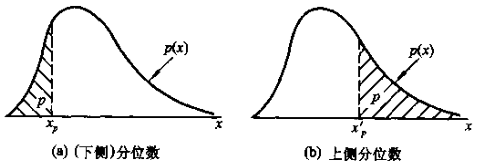
\includegraphics[width=0.7\linewidth]{../../Ptmst/figure/2-7-1}
	\caption{分位数与上侧分位数的区别}
	\label{fig:2-7-1}
\end{figure}

要善于区分分位数与上侧分位数的差别,本书指定用分位数表,而有一些书使用的是上侧分位数表,无论用什么表,书中都有说明.

分位数与上侧分位数是可以相互转换的,其转换公式如下.

\begin{equation}
x_{p}^{\prime}=x_{1-p} ; \quad x_{p}=x_{1-p}^{\prime} \label{eq:2.7.6}
\end{equation}

\begin{example}
	标准正态分布$ N(0,1) $的$ p $分位数记为 $u_{p}$ ,它是方程
	\[
	\Phi\left(u_{p}\right)=p
	\]
	的唯一解,其解为 $u_{p}=\Phi^{-1}(p)$ ,其中 $\Phi^{-1}(\cdot)$ 是标准正态分布函数的反函数.利用标准正态分布函数表(见附表2),我们可由$ p $查得 $u_{p}$ 。譬如 $u_{0.95}=1.96$ .由于标准正态分布的密度函数是偶函数,故其分位数有如下性质:
	
	\begin{itemize}
		\item 当$ p<0.5 $时, $u_{p}<0$ .
		\item 当$ p>0.5 $时,$u_{p}>0$ .
		\item 当$ p=0.5 $时, $u_{0.5}=0$ .
		\item 当 $p_{1}<p_{2}$ 时, $u_{p_{1}}<u_{p_{2}}$ .
		\item 对任意的$ p $,有 $u_{p}=-u_{1-p}$ .
	\end{itemize}
	
	又由定理2.5.1可知:一般正态分布 $N\left(\mu, \sigma^{2}\right)$ 的$ p $分位数 $x_{p}$ 是方程
	
	\[
	\Phi\left(\frac{x_{p}-\mu}{\sigma}\right)=p
	\]
	的解,所以由
	
	\[
	\frac{x_{p}-\mu}{\sigma}=u_{p}
	\]
	可得 $x_{p}$ 与 $u_{p}$ 的关系式
	
	\begin{equation}
	x_{p}=\mu+\sigma u_{p} \label{eq:2.7.7}
	\end{equation}
	譬如正态分布 $N\left(10,2^{2}\right)$ 的$ 0.95 $分位数为
	\[
	x_{0.95}=10+2 u_{0.95}=10+2 \times 1.96=13.92
	\]
\end{example}

分位数在统计中经常被使用,特别对统计中常用的三大分布: $\chi^{2}$ 分布、$ t $分布和$ F $分布,都特地编制了它们的分位数表.以后分别以 $\chi_{\mathrm{a}}^{2}(n), t_{\alpha}(n) , F_{a}(n, m) $ 记这些分布的 $\alpha$ 分位数.例 $\alpha=0.05, n=10, m=15$ 时,查附表3、附表4、附表5,可得

\[
\chi_{1-\alpha}^{2}(n)=18.307 ; \quad t_{1},_{a}(n)=1.8125 ; \quad F_{1-a}(n, m)=2.54
\]

譬如,记某种轴承的寿命为$ T $, $t_{p}$ 为此寿命分布的$ p $分位数,则 $t_{0.1}=1000 (\mathrm{h}) $ ,表明此种轴承中约有$ 90\% $寿命超过1000小时.若记另一种轴承的寿命为$ Z $,$ p $分位数为 $\boldsymbol{z}_{p}$ 。 则当 $z_{0.1}=1500(\mathrm{h})$ 时,从$ 0.1 $的分位数上说明后者的质量比前者更高一些.

\subsection{中位数}

\begin{definition}
	设连续随机变量$ X $的分布函数为$ F(x) $,密度函数为$ p(x) $.
	称$ p=0.5 $时的$ p $分位数 $x_{0.5}$ 为此分布的中位数,即 $x_{0.5}$ 满足
	
	\begin{equation}
	F\left(x_{0.5}\right)=\int_{-\infty}^{x_{0}} p(x) \mathrm{d} x=0.5 \label{eq:2.7.8}
	\end{equation}
	
\end{definition}

中位数的图形见下面图l~\ref{fig:2-7-2}.

\begin{figure}
	\centering
	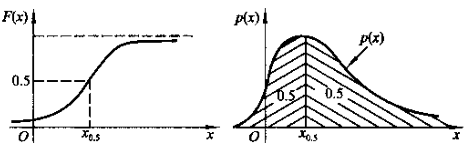
\includegraphics[width=0.7\linewidth]{../../Ptmst/figure/2-7-2}
	\caption{连续随机变量的中位数}
	\label{fig:2-7-2}
\end{figure}

中位数与均值一样都是随机变量位置的特征数,但在某些场合可能中位数比均值更能说明问题.譬如,某班级学生的考试成绩的中位数为80分,则表明斑级中的有一半同学的成绩低于80分,另一半同学的成绩高于80分.而如果考试成绩的均值是80分,则无法得出如此明确的结论.

又譬如,记$ X $为$ A $国人的年龄,$ Y $为$ B $国人的年龄, $x_{0.5}$ 和 $y_{0.5}$ 分别为$ X $和$ Y $的中位数,则$x_{0.5}=40(\text{虽})$说明$ A $国约有一半的人年龄小于等于40岁、一半的人年龄大于等于40岁.而$y_{0.5}=50(\text{岁})$则说明$ B $国更趋于老龄化.

\begin{example}
	指数分布 $E x p(\lambda)$ 的中位数 $x_{0.5}$ 是方程
	
	\[
	1-\mathrm{e}^{-\lambda x 0.5}=0.5
	\]
	的解,解之得
	\[
	x_{0.5}=\frac{\ln 2}{\lambda}
	\]
	
	假如,某城市电话的通话时间$ X(min) $服从均值$ E(X)=2(min) $的指数分布,此时由 $\lambda=0.5$ 可得中位数为
	
	\[
	x_{0.5}=\frac{\ln 2}{0.5}=1.39(\min )
	\]
	它表明:该城市中约有一半的电话在$ 1.39min $内结束,另一半的通话时间超过$ 1.39 min $.
\end{example}

\subsection{偏度系数}

\begin{definition}
	设随机变量$ X $的三阶矩存在,则称比值
	\begin{equation}
	\beta_{1}=\frac{E(X-E(X))^{3}}{\left[E(X-E(X))^{2}\right]^{3 / 2}}=\frac{\nu_{3}}{\left(\nu_{2}\right)^{3 / 2}} \label{eq:2.7.9}
	\end{equation}
	为$ X $的分布的偏度系数,简称偏度.
	
\end{definition}

偏度系数可以描述分布的形状特征,其取值的正负反映的是

\begin{itemize}
	\item 当 $\beta_{1}>0$ 时,分布为正偏或右偏,见图~\ref{fig:2-7-3}(a)
	\item 当 $\beta_{1}=0$ 时,分布关于其均值$ E(X) $对称,见图~\ref{fig:2-7-3}(b).
	\item 当 $\beta_{1}<0$ 时,分布为负偏或左偏,见图~\ref{fig:2-7-3}.
\end{itemize}

\begin{figure}
	\centering
	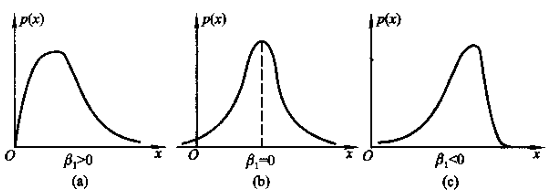
\includegraphics[width=0.7\linewidth]{2-7-3}
	\caption{三种不同偏度的分布}
	\label{fig:2-7-3}
\end{figure}


譬如,正态分布 $N\left(\mu, \sigma^{2}\right)$ 是关于其均值 $E(X)=\mu$ 是对称的,所以正态分布的偏度 $\beta_{1}=0$ .

\subsection{峰度系数}

\begin{definition}
	设随机变量$ X $的四阶矩存在,则称比值
	
	\begin{equation}
	\beta_{2}=\frac{E(X-E(X))^{4}}{\left[E(X-E(X))^{2}\right]^{2}}-3=\frac{\nu_{4}}{\left(\nu_{2}\right)^{2}}-3 \label{eq:2.7.10}
	\end{equation}
	为$ X $的分布的峰度系数,简称峰度.
\end{definition}

峰度系数也是用于描述分布的形状特征,但峰度系数与偏度系数的差别是:
偏度系数刻画的是分布的对称性,而峰度系数刻画的是分布的峰峭性.

峰度系数把正态分布的峰峭性作为标准,因为正态分布 $N\left(\mu, \sigma^{2}\right)$ 的四阶中心矩为 $\nu_{4}=3 \sigma^{4}$ ,所以其峰度系数为

\[
\beta_{2}=\frac{\nu_{4}}{\left(\nu_{2}\right)^{2}}-3=\frac{3 a^{4}}{\sigma^{4}}-3=0
\]

这说明:任一正态分布的峰度 $\beta_{2}=0$ .

可见,这里谈论的“峰度”不是指密度函数的峰值高低,那么“峰度”的含义到底是什么呢?或者换句话说,我们应该如何刻画密度函数的峰峭性呢?我们知道从图形上看密度函数曲线下的面积等于1,若随机变量取值较集中,则其密度函数的峰值必高无疑,所以密度函数峰值的高低含有随机变量取值的集中程度.为了消除这个因素,我们不妨考察“标准化”后的分布的峰峭性,即用

\[
X^{*}=\frac{X-E(X)}{\sqrt{\operatorname{Var}(X)}}
\]
的四阶原点矩 $E\left[\left(X^{*}\right)^{4}\right]$ 考察密度函数的蜂值,再考虑到任一标准正态分布的四阶原点矩等于3,所以就有了以上峰度系数的定义。

综上所述,一个分布的峰度系数 $\beta_{2}$ 反映了以下情况:

\begin{itemize}
	\item 当 $\beta_{2}<0$ 时,则标准化后的分布形状比标准正态分布更平坦,称为低峰度.
	\item 当 $\beta_{2}=0$ 时,则标准化后的分布形状与标准正态分布相当
	\item 当 $\beta_{2}>0$ 时,则标准化后的分布形状比标准正态分布更尖峭,称为高峰度.
\end{itemize}

\begin{example}
	\begin{enumerate}
		\item 均匀分布$ U(a,b) $的密度函数很平坦,其峰度系数 $\beta_{2}= -1.2 $ .可以预计,当一个分布的峰度 $\beta_{2}<-1.2$ 时,其密度函数会呈$ U $形.
		\item 指数分布 $E x p(\lambda)$ 的峰度系数 $\beta_{2}=6$ ,所以指数分布比正态分布更尖峭.
		\item 伽玛分布 $G a(a, \lambda)$ 的偏度系数 $\beta_{1}=2 / \sqrt{\alpha}$ ,峰度系数 $\beta_{2}=6 / \alpha$ ,可见伽玛分布 $G a(\alpha, \lambda)$ 的偏度与峰度只与形状参数 $\alpha$ 有关,而与尺度参数 $\lambda$ 无关.且 $\alpha$  越大, $\beta_{1}$ 与 $\beta_{2}$ 。越小,特别当 $\alpha$  很大时, $\beta_{1}$ 与 $\beta_{2}$ 越接近于零,密度函数越近似于正态密度函数(见图~\ref{fig:2-5-5}).
	\end{enumerate}
\end{example}

\begin{center}
	\textbf{习题2.7}
\end{center}

1.设 $X \sim U(a, b)$ ,对$ k=1,2,3,4 $,求 $\mu_{k}=E\left(X^{k}\right) \leftrightarrows v_{k}=E(X-E(X))^{k}$ .进一步求此分布的偏度系数和峰度系数.

2.设 $X \sim U(0, a)$ ,求此分布的变异系数.

3.设 $X \sim G a(\alpha, \lambda)$ ,对$ k=1,2,3 $,求 $\mu_{k}=E\left(X^{k}\right)$ 与 $\nu_{k}=E(X-E(X))^{k}$ .

4.设 $X-\operatorname{Exp}(\lambda)$ ,对$ k=1,2,3,4 $,求: $\mu_{k}=E\left(X^{k}\right)$ 与 $\nu_{k}=E(X-E(X))^{k}$ .进一步求此分布的变异系数、偏度系数和峰度系数.

5.设随机变量$ X $服从正态分布$ N(10,9) $,试求 $x_{0.1}$ 和 $x_{0.9}$ 

6.设 $Y=\ln X$ ,且 $Y \sim N\left(\mu, \sigma^{2}\right)$ .试求 $x_{0.5}$ .

7.设随机变量$ X $服从双参数威布尔分布,其分布函数为
\[
F(x)=1-\exp \left\{-\left(\frac{x}{\eta}\right)^{m}\right\}, \quad x>0
\]
其中 $\eta>0, m>0$ .试写出该分布的$ p $分位数 $x_{p}$ 的表达式,且求出当 $m=1.5, \eta=1000$ 时的 $x_{0.1}, x_{0.5}, x_{0.8}$ 的值.

8.自由度为2的 $\chi^{2}$ 分布的密度函数为

\[
p(x)=\frac{1}{2} e^{\frac{x}{2}}, \quad x>0
\]

试求出其分布函数及分位数 $x_{0.1}, x_{0.5}, x_{0.8}$ .

9.设随机变量$ X $的分布密度函数$ p(x) $关于$ c $点是对称的,且$ E(X) $存在,试证

\begin{enumerate}
	\item 这个对称点c既是均值又是中位数,即E(X)=x05=c;
	\item 如果$ c=0 $,则 $x_{p}=-x_{1-p}$ .
\end{enumerate}(1)
(2

10.试证随机变量$ X $的偏度系数与峰度系数对位移和改变比例尺是不变的,即对任意的实数 $a, b(b \neq 0), Y=(X-a) / b$ 与$ X $有相同的偏度系数与峰度系数.

